\chapter{连续时间随机过程}
\label{chap:continuous-time-stochastic-processes}

设想三台记录仪同时工作。第一台记录服务器收到请求的时刻，请求可以在任何一个实数时刻到来，每来一个，计数就跳高一格；第二台跟踪水中一粒花粉的横坐标，读数从不跳变，却在任意短的时间里都在抖动；第三台记录一个受持续扰动的温度，扰动的大小还取决于温度本身。三条记录都以连续时间为索引，但前一条是跳跃路径，后两条是连续路径，第三条还把噪声和未知状态缠在了一起。

上一章已经为按轮次更新的随机序列回答了一组问题：一步转移怎样决定多步规律，给定历史后增量有没有平均漂移，何时停止仍保留期望关系，长期分布和时间平均是否收敛，以及怎样用随机序列计算积分和寻找方程的根。把时间换成实数轴以后，这些问题都还在，但每一个都多出一层困难。没有“下一步”，转移只能用任意时长的核和短时间变化率来描述；任意短的区间里都有噪声，累计噪声需要新的积分；停时可以取不可数多个值，离散证明里“按每个可能取值求和”的做法失效；单个时刻上的零概率例外也不能再无条件地合并。

本章沿着与上一章对应的问题线展开。我们先构造Poisson过程与Brownian运动这两类基本路径，并交代不可数时刻带来的版本、滤过和停时条件；随后分别研究条件未来（转移半群与生成元）和条件均值（鞅、停止与补偿）。有了这两种结构，才能定义对随机驱动的累计——Itô积分，并用Itô公式计算状态函数的变化；再让系数依赖未知状态，就得到随机微分方程。方程的解可以逐路径研究，也可以通过生成元转成关于期望、密度和首次到达的确定性方程；两种视角共同回答长期行为与稳定性问题。

最后四节转向计算和近似。数值模拟需要分清路径误差与期望误差；采样积分把一条长时间运行的随机路径当作求平均的工具，连续时间随机逼近则让噪声随时间压低以逼近方程的根，二者使用相同的过程工具却追求相反的长期行为。最后一节比较整条路径的分布，说明随机游走何时可以近似为扩散，这为前面的离散模拟与连续模型之间的关系提供进阶的极限依据。

\section{连续时间的随机路径}
\label{sec:ctsp-paths}

第~\ref{chap:stochastic-processes-and-sample-paths}章把随机过程写成共同概率空间上的随机变量族$(X_t)_{t\in\mathbb T}$，并区分了固定时刻的随机变量与固定实现的样本路径。本节把索引集取为$\mathbb T=[0,\infty)$。我们先构造两个可以直接计算的模型：按事件跳跃的Poisson过程，以及处处连续却处处抖动的Brownian运动；再回头处理不可数时刻带来的问题，即路径版本、信息结构和停时需要满足哪些额外条件。这些条件不是为抽象而抽象，后面每一个结论在使用它们时都会指出它们承担的作用。

\subsection{事件到达与Poisson过程}
\label{sec:ctsp-poisson}

\paragraph{从等待时间到计数路径}
想象一台服务器，请求一个接一个地到来。最简单的模型只规定相邻请求之间的等待时间：它们相互独立，都服从速率为$\lambda>0$的指数分布。指数分布的特点是无记忆：已经等了$s$个单位时间而请求仍未到来，再等至少$u$的概率仍是
\[
  \mathbb P(E>s+u\mid E>s)=\frac{e^{-\lambda(s+u)}}{e^{-\lambda s}}=e^{-\lambda u}=\mathbb P(E>u).
\]
因此服务器“已经空闲了多久”不提供任何关于下一次到达的信息，这正是“事件以恒定速率随机发生”的数学表达。

设$E_1,E_2,\ldots$独立同分布于$\operatorname{Exp}(\lambda)$。第$k$次到达时刻和到时刻$t$为止的到达次数分别为
\begin{equation}
  T_k=E_1+\cdots+E_k,\qquad
  N_t=\#\{k\geq1:T_k\leq t\}.
  \label{eq:ctsp-poisson-construction}
\end{equation}
同一个随机机制因此有三种描述：等待时间序列、到达时刻序列和计数路径。图~\ref{fig:ctsp-poisson-three-views}把它们画在同一条时间轴上。读者可以沿竖直方向对照：每段等待结束的地方就是一个到达时刻，计数路径恰好在那里向上跳一格，其余时间保持水平。

\begin{figure}[htbp]
  \centering
  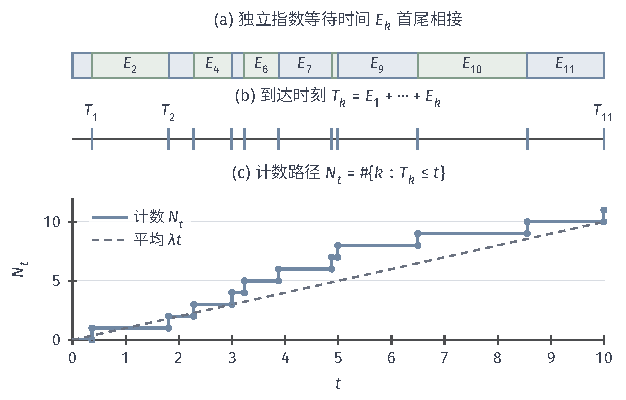
\includegraphics[width=105mm]{figures/03-optimization-evolution-and-signals/02-processes-and-trajectory-evolution/tikz/ctsp-poisson-three-views/figure.pdf}
  \caption{同一Poisson机制的三种描述（固定随机种子的一次实现，$\lambda=1$，时段$[0,10]$）。(a)独立指数等待时间首尾相接，蓝绿交替只为区分相邻段；(b)每段末端是一个到达时刻；(c)计数路径在到达时刻跳高一格，实心点是跳后的取值，空心点是跳前的左极限，虚线是平均计数$\lambda t$。}
  \label{fig:ctsp-poisson-three-views}
\end{figure}

计数路径有几条一眼可见的性质：$N_0=0$，路径非减、取非负整数、每次跳跃的高度为一，并且在每个跳跃时刻取跳后的值，即右连续；在每个时刻左侧都有极限$N_{t-}=\lim_{s\uparrow t}N_s$，跳跃量记为$\Delta N_t=N_t-N_{t-}$。另一条性质需要论证：有限时段内只有有限次跳跃。由强大数律，$T_k/k\to1/\lambda$几乎必然，所以$T_k\to\infty$，任意有界区间$[0,t]$只包含有限个到达时刻。没有这条性质，计数在有限时间内就可能变成无穷。

\paragraph{计数的Poisson规律}
从等待时间出发，可以算出固定时刻计数的分布。$T_k$是$k$个独立指数变量之和，服从$\operatorname{Gamma}(k,\lambda)$，密度为$f_k(s)=\lambda^ks^{k-1}e^{-\lambda s}/(k-1)!$。由于$\{N_t\geq k\}=\{T_k\leq t\}$，
\[
  \mathbb P(N_t=k)=\mathbb P(T_k\leq t)-\mathbb P(T_{k+1}\leq t)
  =\int_0^t[f_k(s)-f_{k+1}(s)]\,\mathrm ds .
\]
直接求导可验证$\frac{\mathrm d}{\mathrm ds}\bigl[e^{-\lambda s}(\lambda s)^k/k!\bigr]=f_k(s)-f_{k+1}(s)$，于是
\begin{equation}
  \mathbb P(N_t=k)=e^{-\lambda t}\frac{(\lambda t)^k}{k!},\qquad k=0,1,2,\ldots
  \label{eq:ctsp-poisson-marginal}
\end{equation}
即$N_t\sim\operatorname{Poisson}(\lambda t)$。$k=0$时它就是$\mathbb P(E_1>t)=e^{-\lambda t}$。

单个时刻的分布还不足以描述过程，需要知道不同时间段的计数怎样联合。无记忆性在这里起关键作用。固定$s$，在事件$\{N_s=k\}$上，已经发生的到达是$T_1,\ldots,T_k$，下一次到达的剩余等待$T_{k+1}-s$满足
\[
  \mathbb P(T_{k+1}-s>u\mid T_1,\ldots,T_k,\ N_s=k)=e^{-\lambda u},
\]
因为它是$E_{k+1}$在已知$E_{k+1}>s-T_k$条件下超出部分的分布；其后的$E_{k+2},E_{k+3},\ldots$又与过去无关。所以从时刻$s$重新计时，未来的等待时间仍是一列独立的$\operatorname{Exp}(\lambda)$变量，并且独立于$s$以前的记录。

\begin{theorem}[Poisson过程的增量]
  \label{thm:ctsp-poisson-increments}
  由式~\eqref{eq:ctsp-poisson-construction}构造的计数过程，对任意$0\leq s<t$，增量$N_t-N_s$独立于$\sigma(N_u:u\leq s)$，并服从$\operatorname{Poisson}(\lambda(t-s))$。因而对任意$0\leq t_0<t_1<\cdots<t_n$，各段增量相互独立。
\end{theorem}

\begin{proof}
上面的论证说明，$(N_{s+u}-N_s)_{u\geq0}$由一列与过去独立的$\operatorname{Exp}(\lambda)$等待时间按同样的规则生成，因此它与$(N_u)_{u\geq0}$同分布且独立于$\sigma(N_u:u\leq s)$。取$u=t-s$并用式~\eqref{eq:ctsp-poisson-marginal}得到增量分布。对多个时间段，从最后一段开始依次使用这一独立性，即得各段增量相互独立。把无记忆性写成严格的条件分布等式需要对$k$和$T_1,\ldots,T_k$的取值积分，细节见Kallenberg的概率论教材。
\end{proof}

条件分布形式的细节可参考文献\scite{math-kallenberg2021probability}。

这一定理把构造得到的对象与通常的公理式定义连接起来。以后研究随机积分时，还要允许滤过比计数自身的历史更大，因此我们按下面的形式使用Poisson过程。

\begin{definition}[Poisson过程]
  \label{def:ctsp-poisson-process}
  给定速率$\lambda>0$和滤过$(\mathcal F_t)_{t\geq0}$，适应的计数过程$N$称为相对于该滤过的\term{Poisson过程}（Poisson process），若$N_0=0$，路径右连续、非减、取整数值且每次跳跃高度为一，并且对$0\leq s<t$，$N_t-N_s$独立于$\mathcal F_s$，服从$\operatorname{Poisson}(\lambda(t-s))$。
\end{definition}

速率$\lambda$描述单位时间内的平均事件数，即$\mathbb EN_t=\lambda t$；它不是概率。从式~\eqref{eq:ctsp-poisson-marginal}在$h\downarrow0$时展开，
\[
  \mathbb P(N_{t+h}-N_t=1)=\lambda h+O(h^2),\qquad
  \mathbb P(N_{t+h}-N_t\geq2)=O(h^2).
\]
只有在短时间$h$内，$\lambda h$才近似为发生一次事件的概率。例如每分钟平均三个请求时，一分钟内至少来一个请求的概率是$1-e^{-3}\approx0.95$，而不是$3$；把$\lambda$直接当成“每步转移概率”的离散化，在$\lambda h$不小时会产生明显偏差。

\paragraph{复合Poisson过程与逐事件模拟}
很多应用中，事件的影响不是固定的一格。保险公司每收到一笔理赔，金额是随机的；股票价格在消息到达时跳变，跳幅可正可负。设$J_1,J_2,\ldots$独立同分布，并独立于计数过程$N$，定义
\begin{equation}
  C_t=\sum_{k=1}^{N_t}J_k ,
  \label{eq:ctsp-compound-poisson}
\end{equation}
称为\term{复合Poisson过程}（compound Poisson process）。它的路径仍在到达时刻跳跃，只是跳幅由标记$J_k$给出，见图~\ref{fig:ctsp-compound-poisson}。

\begin{figure}[htbp]
  \centering
  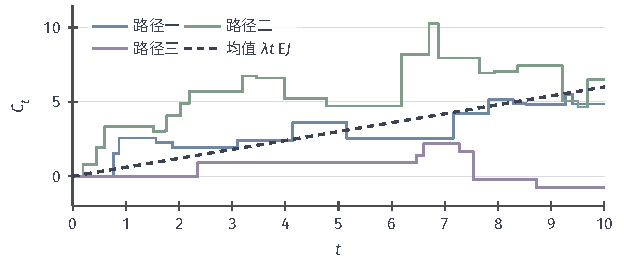
\includegraphics[width=105mm]{figures/03-optimization-evolution-and-signals/02-processes-and-trajectory-evolution/tikz/ctsp-compound-poisson/figure.pdf}
  \caption{复合Poisson过程的三条独立路径。到达速率$\lambda=1.5$，跳幅$J_k\sim\mathcal N(0.4,1)$，固定随机种子。路径在到达之间保持水平，跳幅可正可负；虚线为均值$\lambda t\,\mathbb EJ=0.6t$。单条路径可以长时间偏离均值线，均值只描述大量路径的平均。}
  \label{fig:ctsp-compound-poisson}
\end{figure}

先给定$N_t$再求平均，可以得到均值和方差。给定$N_t=n$时，$C_t$是$n$个独立标记之和，因而
\[
  \mathbb E[C_t\mid N_t]=N_t\,\mathbb EJ_1,\qquad
  \operatorname{Var}(C_t\mid N_t)=N_t\operatorname{Var}(J_1).
\]
由全期望公式与全方差公式，在$\mathbb EJ_1^2<\infty$时，
\begin{equation}
  \mathbb EC_t=\lambda t\,\mathbb EJ_1,\qquad
  \operatorname{Var}(C_t)=\lambda t\operatorname{Var}(J_1)+(\mathbb EJ_1)^2\operatorname{Var}(N_t)=\lambda t\,\mathbb EJ_1^2 .
  \label{eq:ctsp-compound-moments}
\end{equation}
方差中出现的是二阶矩$\mathbb EJ_1^2$而不是$\operatorname{Var}(J_1)$，多出的部分来自事件个数本身的随机性。

\begin{example}[十天的理赔总额]
  \label{ex:ctsp-claims}
  理赔以每天$\lambda=2$笔的速率到达，每笔金额的均值为$3$、二阶矩为$13$（方差为$4$）。十天的理赔总额$C_{10}$满足$\mathbb EC_{10}=2\times10\times3=60$，$\operatorname{Var}(C_{10})=2\times10\times13=260$。若误用$\lambda t\operatorname{Var}(J_1)=80$作为方差，标准差会从约$16.1$低估为约$8.9$。
\end{example}

复合Poisson过程可以精确模拟，不需要时间网格：依次抽取等待时间$E_1,E_2,\ldots$，直到累计和超过时域$T$，再为每个到达抽取一个标记并累加。计算量与事件数成正比，期望为$\lambda T$；输出的跳时与跳幅都与模型分布完全一致。相比之下，把时间切成步长$h$、每步以概率$\lambda h$决定是否发生一次事件，会忽略一步内的多次事件并把跳时对齐到网格上；这种近似误差将在第~\ref{sec:ctsp-jump-simulation}节与精确的事件驱动模拟比较。

\subsection{Brownian运动与路径波动}
\label{sec:ctsp-brownian}

\paragraph{从随机游走到连续波动}
现在换到第二台记录仪：水中的花粉粒被大量水分子撞击，每一次撞击都很微小，累计起来却使它不停地游走。离散模型是随机游走：每隔$\Delta t$走一步，步长为$\pm a$，各步独立且等可能。到时刻$t=n\Delta t$，位置的方差为$na^2=ta^2/\Delta t$。要让固定时刻的方差在$\Delta t\to0$时既不消失也不发散，步长必须按$a=\sqrt{\Delta t}$缩放，此时方差恰好为$t$。

这个$\sqrt{\Delta t}$尺度是理解后面一切现象的钥匙。时间缩短为原来的四分之一，位移只缩小为原来的一半，所以路径越看越陡。由中心极限定理，固定时刻的位置趋于$\mathcal N(0,t)$；整条折线路径的极限则需要第~\ref{sec:ctsp-donsker}节的Donsker定理。这里不走极限路线，而是直接规定极限对象应当具有的性质。

\begin{definition}[标准Brownian运动]
  \label{def:ctsp-brownian-motion}
  实值过程$(W_t)_{t\geq0}$称为标准\term{Brownian运动}（Brownian motion），若
  \begin{enumerate}
    \item $W_0=0$几乎必然；
    \item 对任意$0\leq t_0<t_1<\cdots<t_n$，增量$W_{t_1}-W_{t_0},\ldots,W_{t_n}-W_{t_{n-1}}$相互独立；
    \item 对$0\leq s<t$，$W_t-W_s\sim\mathcal N(0,t-s)$；
    \item 样本路径几乎必然连续。
  \end{enumerate}
  相对于滤过$(\mathcal F_t)$使用时，还要求$W$适应，且对$s<t$，$W_t-W_s$独立于$\mathcal F_s$。$m$维标准Brownian运动$\bm W=(W^{(1)},\ldots,W^{(m)})^\top$由$m$个相互独立的标准Brownian运动组成，其增量$\bm W_t-\bm W_s\sim\mathcal N(\bm0,(t-s)\bm I_m)$。
\end{definition}

前三条只涉及有限个时刻的联合分布。写$s\leq t$，由$W_t=W_s+(W_t-W_s)$及增量独立，
\begin{equation}
  \mathbb E W_t=0,\qquad
  \operatorname{Cov}(W_s,W_t)=\mathbb EW_s^2=\min(s,t).
  \label{eq:ctsp-brownian-covariance}
\end{equation}
任意有限个取值$(W_{t_1},\ldots,W_{t_n})$都是独立高斯增量的线性变换，所以联合高斯，其规律完全由协方差$\min(s,t)$决定。

\paragraph{连续版本的存在}
定义中的第四条与前三条性质不同。第~\ref{chap:stochastic-processes-and-sample-paths}章已经说明，相容的有限维分布可以通过Kolmogorov扩张定理得到乘积空间上的过程，但有限维分布并不约束路径在不可数多个时刻上的整体形状；第~\ref{sec:ctsp-path-versions}节会用一个具体例子说明这一点。所以“增量独立且高斯”是分布性质，“路径连续”是另外选出的版本性质，后者需要单独论证。

论证的工具是该章的Kolmogorov连续性准则：若存在$p,\beta,C>0$，使$\mathbb E|X_t-X_s|^p\leq C|t-s|^{1+\beta}$对紧区间上的所有$s,t$成立，则$X$有连续修改，且其路径对任意$\gamma<\beta/p$是$\gamma$阶Hölder连续的。对Brownian增量，$W_t-W_s\sim\mathcal N(0,|t-s|)$给出
\[
  \mathbb E|W_t-W_s|^{2m}=(2m-1)!!\,|t-s|^m,\qquad m=1,2,\ldots
\]
取$p=2m$、$\beta=m-1$，准则对$m\geq2$适用，给出阶数$\gamma<(m-1)/(2m)$的Hölder连续版本。令$m\to\infty$，得到下面的结论。

\begin{theorem}[Brownian运动的存在与路径正则性]
  \label{thm:ctsp-brownian-existence}
  存在满足定义~\ref{def:ctsp-brownian-motion}的过程。其几乎每条路径在每个有界区间上对任意$\gamma<1/2$都是$\gamma$阶Hölder连续的。
\end{theorem}

\begin{proof}
协方差函数$\min(s,t)$半正定：对任意实数$c_i$与时刻$t_i$，$\sum_{i,j}c_ic_j\min(t_i,t_j)=\int_0^\infty\bigl(\sum_ic_i\mathbb I\{u\leq t_i\}\bigr)^2\,\mathrm du\geq0$。因此均值零、协方差$\min(s,t)$的高斯有限维分布相容，Kolmogorov扩张给出一个过程，它满足定义中的前三条。上面的矩计算对每个$m\geq2$给出Hölder连续修改；对可数个$m$取共同的修改（两个连续修改不可区分，见第~\ref{sec:ctsp-path-versions}节），就得到对所有$\gamma<1/2$同时成立的版本。修改不改变有限维分布，所以前三条仍然成立。
\end{proof}

\paragraph{尺度不变与粗糙路径}
由增量方差的线性尺度，可以检查Brownian运动的自相似：对任意$c>0$，
\begin{equation}
  \widetilde W_t=c^{-1/2}W_{ct}
  \label{eq:ctsp-brownian-scaling}
\end{equation}
仍是标准Brownian运动。它从零出发，增量独立，$\widetilde W_t-\widetilde W_s\sim\mathcal N(0,c(t-s)/c)=\mathcal N(0,t-s)$，路径连续性也由原路径继承。

图~\ref{fig:ctsp-brownian-zoom}把这一性质画了出来。把同一条路径在$[0,1/4]$上的一段横向拉伸四倍、纵向放大两倍，得到的图形与原图在统计意义上无法区分；再放大一次仍然如此。光滑曲线在放大后会越来越接近一条直线，这正是导数存在的几何含义。Brownian路径无论放大多少倍都不会变直。

\begin{figure*}[htbp]
  \centering
  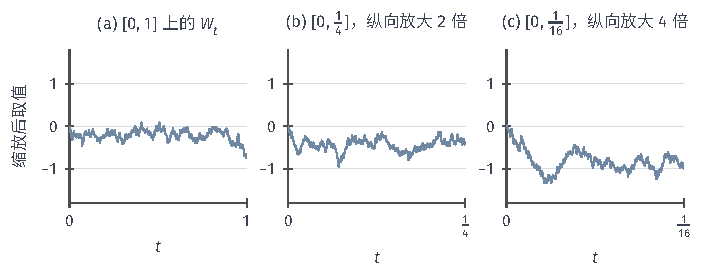
\includegraphics[width=119mm]{figures/03-optimization-evolution-and-signals/02-processes-and-trajectory-evolution/tikz/ctsp-brownian-zoom/figure.pdf}
  \caption{Brownian路径的自相似。用$2^{16}$个独立增量$\mathcal N(0,2^{-16})$累计出一条教学路径（固定随机种子）。(a)$[0,1]$上的整条路径；(b)同一路径在$[0,\frac14]$上的一段，横轴拉伸到$[0,1]$，纵轴乘以$2$；(c)$[0,\frac1{16}]$上的一段，纵轴乘以$4$。按$c^{-1/2}W_{ct}$缩放后，三幅图的起伏幅度相当，放大并没有使路径变得平直。每幅图只绘出约$1100$个网格点。}
  \label{fig:ctsp-brownian-zoom}
\end{figure*}

尺度不变也给出差商的量级。$(W_{t+h}-W_t)/h$服从$\mathcal N(0,1/h)$，标准差$h^{-1/2}$在$h\downarrow0$时发散，所以不能期望在固定时刻存在导数。更强的结论是：以概率一，Brownian路径在任何时刻都不可微。这个结论同时涉及不可数个时刻，不能由逐个固定时刻的计算推出，它的证明见Kallenberg的概率论教材。对后续内容来说，重要的推论是：形如$\mathrm dW_t/\mathrm dt$的“白噪声”不是普通的随机函数，随机微分方程中的$\mathrm dW_t$必须另行解释。

\paragraph{二次变差与总变差}
光滑路径与Brownian路径的差别，可以用两种沿路径的累计量来度量。取$[0,t]$的分割$\pi:0=t_0<t_1<\cdots<t_n=t$，网格宽度$|\pi|=\max_i(t_{i+1}-t_i)$，记$\Delta W_i=W_{t_{i+1}}-W_{t_i}$。考虑平方增量和与绝对增量和
\[
  Q_\pi=\sum_{i}(\Delta W_i)^2,\qquad
  V_\pi=\sum_i|\Delta W_i| .
\]

\begin{theorem}[Brownian运动的二次变差]
  \label{thm:ctsp-brownian-qv}
  对$[0,t]$上任意一列网格宽度趋于零的确定分割$\pi_n$，$Q_{\pi_n}\to t$在$L^2$中成立，从而依概率成立。
\end{theorem}

\begin{proof}
增量独立且$\Delta W_i\sim\mathcal N(0,\Delta t_i)$，所以$\mathbb EQ_\pi=\sum_i\Delta t_i=t$。由正态四阶矩$\mathbb E(\Delta W_i)^4=3(\Delta t_i)^2$，$\operatorname{Var}((\Delta W_i)^2)=2(\Delta t_i)^2$，再由独立性
\[
  \mathbb E(Q_\pi-t)^2=\operatorname{Var}(Q_\pi)=2\sum_i(\Delta t_i)^2\leq2t|\pi| .
\]
网格宽度趋零时右端趋零。
\end{proof}

网格加细时平方增量和的极限称为\term{二次变差}（quadratic variation），记作$[W]_t$；定理说明$[W]_t=t$。二次变差与方差回答的问题不同。方差$\operatorname{Var}(W_t)=t$是在固定时刻对大量实现求平均；二次变差是在一条实现上沿时间累计平方增量，再加细分割。两者在这里数值相同，是Brownian增量方差与时间长度成正比的结果。

绝对增量和的行为完全相反。对等分分割，$\mathbb E|\Delta W_i|=\sqrt{2\Delta t_i/\pi}$，所以$\mathbb EV_\pi=\sqrt{2nt/\pi}\to\infty$。更进一步，路径在每个区间上几乎必然具有无限\term{总变差}（total variation），即所有分割上$V_\pi$的上确界为无穷。理由是：若某条连续路径$x$在$[0,t]$上总变差有限，则
\[
  \sum_i(\Delta x_i)^2\leq\max_i|\Delta x_i|\cdot\sum_i|\Delta x_i|\longrightarrow0,
\]
因为连续函数在紧区间上一致连续，$\max_i|\Delta x_i|\to0$。而定理~\ref{thm:ctsp-brownian-qv}说明，沿一列分割$Q_{\pi_n}\to t$依概率成立，取一个子列便几乎必然收敛到$t>0$。两者矛盾，所以有限总变差的路径只构成零概率集合。对所有有理端点区间取可数并，结论对所有区间同时成立。

图~\ref{fig:ctsp-quadratic-variation}沿二进分割比较了这两个累计量。Brownian路径的平方增量和停在$1$附近，绝对增量和则按$\sqrt n$增长；光滑路径$\sin(2\pi t)$恰好相反，平方增量和趋零，绝对增量和趋于有限的总变差$4$。

\begin{figure}[htbp]
  \centering
  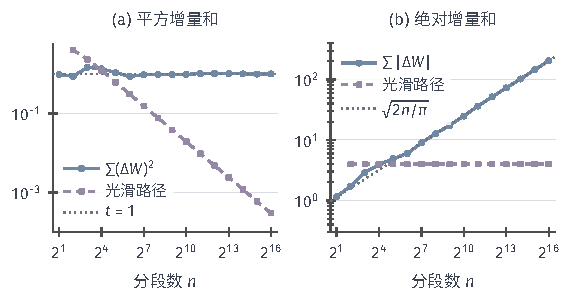
\includegraphics[width=97mm]{figures/03-optimization-evolution-and-signals/02-processes-and-trajectory-evolution/tikz/ctsp-quadratic-variation/figure.pdf}
  \caption{同一条Brownian教学路径（$2^{16}$个独立增量，固定随机种子）与光滑路径$\sin(2\pi t)$在$[0,1]$上沿二进分割的累计量，双轴均为对数刻度。(a)平方增量和：Brownian路径趋近二次变差$1$，光滑路径按$1/n$趋零；(b)绝对增量和：Brownian路径沿参考线$\sqrt{2n/\pi}$（期望值）增长，光滑路径趋于总变差$4$。}
  \label{fig:ctsp-quadratic-variation}
\end{figure}

这两条结论共同决定了第~\ref{sec:ctsp-stochastic-integration}节的走向。无限总变差意味着不能把$\int H_t\,\mathrm dW_t$当作逐路径的Stieltjes积分；非零二次变差意味着Taylor展开中的二阶项$\frac12f''(W)(\Delta W)^2$累计后不会消失，普通链式法则需要修正。

\subsection{路径版本与连续时间信息}
\label{sec:ctsp-path-versions}

\paragraph{不可数时刻上的零概率例外}
离散时间中有一条常用的推理：若对每个$n$，事件$\{X_n=Y_n\}$的概率为一，则$\{X_n=Y_n\text{ 对所有 }n\}$的概率也为一，因为可数个零概率集合的并仍是零概率集合。时间连续以后，时刻有不可数多个，这条推理不再成立。

\begin{example}[随机位置的单点尖峰]
  \label{ex:ctsp-single-spike}
  设$\tau\sim\operatorname{Uniform}(0,1)$，令$X_t\equiv0$，$Y_t=\mathbb I\{t=\tau\}$，$t\in[0,1]$。对每个固定的$t$，$\mathbb P(X_t\neq Y_t)=\mathbb P(\tau=t)=0$，所以两个过程的有限维分布完全相同。但对每个结果$\omega$，$Y$的路径都在$\tau(\omega)$处取值$1$，于是$\mathbb P(X_t=Y_t\text{ 对所有 }t)=0$。$X$的路径连续，$Y$的路径处处不连续于$\tau$。
\end{example}

图~\ref{fig:ctsp-path-versions}画出了一次实现。有限维分布无法区分两者，所以“Brownian运动的路径是否连续”不是有限维分布能回答的问题，只能在同分布的版本中挑出路径性质合适的那一个。

\begin{figure}[htbp]
  \centering
  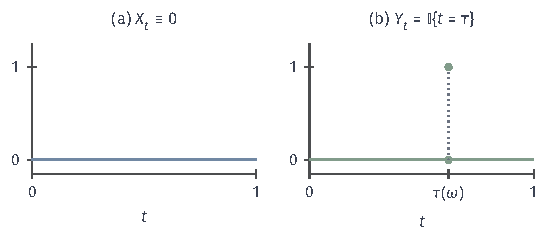
\includegraphics[width=100mm]{figures/03-optimization-evolution-and-signals/02-processes-and-trajectory-evolution/tikz/ctsp-path-versions/figure.pdf}
  \caption{有限维分布相同而路径不同（示例~\ref{ex:ctsp-single-spike}的一次实现，图中取$\tau(\omega)=0.62$）。(a)零路径；(b)只在随机时刻$\tau(\omega)$取$1$的路径，实心点为该时刻的取值，空心点表示路径在那里的左右极限仍为$0$。任一固定时刻恰好落在尖峰上的概率为零。}
  \label{fig:ctsp-path-versions}
\end{figure}

第~\ref{chap:stochastic-processes-and-sample-paths}章区分了两种相等。若对每个$t$，$\mathbb P(X_t=Y_t)=1$，称$Y$是$X$的修改；若存在一个概率为一的事件，在其上$X_t=Y_t$对所有$t$同时成立，称两者不可区分。示例中的$Y$是$X$的修改，却与$X$可以区分。路径正则性正好弥补二者之间的缺口。

\begin{lemma}[右连续修改不可区分]
  \label{lem:ctsp-right-continuous-modification}
  若$X$与$Y$互为修改，且两者的路径几乎必然右连续，则$X$与$Y$不可区分。
\end{lemma}

\begin{proof}
令$D=\mathbb Q\cap[0,\infty)$。$D$可数，所以$\mathbb P(X_q=Y_q\text{ 对所有 }q\in D)=1$。对任意$t$取$q_n\in D$，$q_n\downarrow t$，在上述事件与两条路径都右连续的事件之交上，$X_t=\lim X_{q_n}=\lim Y_{q_n}=Y_t$。
\end{proof}

本章的过程都取\term{右连续有左极限}（càdlàg）的版本：每条路径在每个时刻右连续，并且左极限存在。Poisson过程和以后的跳跃过程天然如此，Brownian运动和连续Itô过程则是其中路径连续的特例。引理~\ref{lem:ctsp-right-continuous-modification}保证这样的版本若存在，则在不可区分的意义下唯一。

\paragraph{滤过的正则条件}
信息结构也需要同样的补充。离散时间中，滤过只需逐个时刻递增；连续时间中还要求它在两种意义下“没有缺口”。一是完备：$\mathcal F_0$包含所有概率零集合的子集，这样在零概率集合上修改一个适应过程后仍然适应。二是右连续：$\mathcal F_t=\bigcap_{s>t}\mathcal F_s$，即“在$t$之后任意短时间内就能知道的事”在$t$时已经知道。同时满足两者时称滤过满足\term{通常条件}（usual conditions）。

右连续性的用途在停时中最清楚。设$X$连续适应，$G$是开集，考虑首次进入时刻$\tau=\inf\{t:X_t\in G\}$。在时刻$t$判断“$\tau<t$”只需看$t$之前的有理时刻，所以$\{\tau<t\}\in\mathcal F_t$；判断“$\tau\leq t$”却可能需要看$t$之后一瞬间路径是否进入$G$。右连续滤过使$\{\tau\leq t\}=\bigcap_n\{\tau<t+1/n\}\in\bigcap_n\mathcal F_{t+1/n}=\mathcal F_t$。Brownian运动的自然滤过经过完备化后满足通常条件，Poisson过程亦然\scite{math-kallenberg2021probability}。本章此后默认滤过满足通常条件。

\paragraph{联合可测与可预测}
随时间积分还需要一种联合可测性。积分$\int_0^tX_s\,\mathrm ds$同时用到时间变量与随机结果；即使每个$X_s$都$\mathcal F_s$可测，若$(s,\omega)\mapsto X_s(\omega)$不是联合可测的，积分甚至可能不是随机变量。若对每个$t$，映射$(s,\omega)\mapsto X_s(\omega)$在$[0,t]\times\Omega$上对$\mathcal B([0,t])\otimes\mathcal F_t$可测，称$X$\term{渐进可测}（progressively measurable）。渐进可测保证$\int_0^tX_s\,\mathrm ds$是$\mathcal F_t$可测的，也保证停时处的取值$X_\tau$可测。

右连续适应过程都是渐进可测的。固定$t$，令$X^{(n)}_s=X_{\min\{(k+1)t/2^n,t\}}$，$s\in[kt/2^n,(k+1)t/2^n)$。每个$X^{(n)}$在$[0,t]\times\Omega$上只取有限个$\mathcal F_t$可测的值，对乘积$\sigma$代数可测；右连续性使$X^{(n)}_s\to X_s$逐点成立，极限保持可测性。左连续适应过程同理。

另一种要求来自事件发生的先后。计数路径在到达时刻$T_k$跳跃，跳后的值$N_{T_k}$在跳跃前不可能知道；如果一个系数要在“事件发生前”就确定，它只能使用严格早于当前时刻的信息。由全部左连续适应过程生成的$\sigma$代数称为可预测$\sigma$代数，对它可测的过程称为\term{可预测过程}。它也由形如$(s,u]\times A$、$A\in\mathcal F_s$的矩形生成：在$s$时刻已知事件$A$是否发生，便可决定在$(s,u]$上取什么值。连续适应过程和左极限过程$N_{t-}$都是可预测的，跳后的$N_t$则不是。第~\ref{sec:ctsp-time-jump-integrals}节将说明这一区别怎样决定跳跃积分的均值。

\paragraph{连续时间的停时}
第~\ref{chap:stochastic-processes-and-sample-paths}章与第~\ref{chap:discrete-time-stochastic-processes}章在离散时间中用“每一步都能判断是否已经停止”刻画停时。连续时间把这一要求放到每个实数时刻上。

\begin{definition}[连续时间停时]
  \label{def:ctsp-stopping-time}
  取值于$[0,\infty]$的随机变量$\tau$称为相对于$(\mathcal F_t)$的\term{停时}，若对每个实数$t\geq0$，$\{\tau\leq t\}\in\mathcal F_t$。与之相伴的信息为$\mathcal F_\tau=\{A\in\mathcal F:A\cap\{\tau\leq t\}\in\mathcal F_t\text{ 对所有 }t\geq0\}$。
\end{definition}

下面三个例子分别检查定义所需的适应性、路径正则性与目标集合条件。

第一，连续适应过程首次到达闭集$F$的时刻$\tau_F=\inf\{t:X_t\in F\}$是停时。记$d(x,F)$为点到$F$的距离。由路径连续和$F$闭，$\tau_F\leq t$当且仅当$\inf_{s\in[0,t]}d(X_s,F)=0$；连续性又允许把下确界只取在可数集$(\mathbb Q\cap[0,t])\cup\{t\}$上，因此该事件属于$\mathcal F_t$。若改用跳跃路径，或把闭集换成开集，就需要右连续滤过等额外条件。

第二，Poisson过程的第$k$次到达时刻是停时，因为$\{T_k\leq t\}=\{N_t\geq k\}\in\mathcal F_t$。跳跃路径的事件时刻可以由当前计数判断，不需要路径连续。

第三，作为反例，令$\sigma=\sup\{t\leq1:W_t=0\}$为Brownian运动在$[0,1]$上最后一次回到零的时刻。判断$\sigma\leq t$需要知道$t$之后到$1$为止路径是否再回到零，这依赖未来，所以$\sigma$不是停时。

连续停时可以取不可数多个值，这使离散时间中“按停时取值分解再求和”的证明无法直接使用。下面的离散化从上方逼近停时，是本章反复使用的桥梁：令
\begin{equation}
  \tau_n=\frac{\lfloor2^n\tau\rfloor+1}{2^n}\quad(\tau<\infty),\qquad\tau_n=\infty\quad(\tau=\infty).
  \label{eq:ctsp-dyadic-stopping}
\end{equation}
每个$\tau_n$只取可数多个二进值，并且$\tau_n\downarrow\tau$。它仍是停时：$\tau_n\leq t$等价于$\tau<\lfloor2^nt\rfloor/2^n$，后者属于$\mathcal F_{\lfloor2^nt\rfloor/2^n}\subseteq\mathcal F_t$。从上方逼近是必要的，向下取整得到的随机时刻需要“提前知道”停止，一般不是停时。停止后的Markov规律与鞅期望将分别在第~\ref{sec:ctsp-strong-markov}节和第~\ref{sec:ctsp-optional-sampling}节借助这一逼近建立。

\section{条件未来与局部转移}
\label{sec:ctsp-markov}

第~\ref{chap:discrete-time-stochastic-processes}章用一步转移核$P$描述Markov链：给定当前状态，下一步的条件分布是$P(x,\cdot)$，$n$步转移是核的$n$次复合。连续时间没有“一步”，本节先把转移推广为任意时长$t$的核族，再用短时间内的变化率——生成元——概括这一族核。有限或可数状态的跳跃链让这些对象都变成可以直接计算的矩阵。最后讨论在随机时刻停止后，过程能否像在固定时刻那样重新开始。

\subsection{转移半群与生成元}
\label{sec:ctsp-semigroup}

\paragraph{任意时长的转移核}
设$X$在可测状态空间$(E,\mathcal E)$中取值，并适应于滤过$(\mathcal F_t)$。若存在一族概率核$P_t$，$t\geq0$，使
\begin{equation}
  \mathbb P(X_{s+t}\in A\mid\mathcal F_s)=P_t(X_s,A)\qquad\text{几乎必然},\quad s,t\geq0,\ A\in\mathcal E,
  \label{eq:ctsp-markov-property}
\end{equation}
就称$X$是相对于该滤过的时间齐次Markov过程，$P_t$称为转移核。条件只依赖经过的时长$t$，不依赖出发时刻$s$；若依赖$s$，就要用双参数核$P_{s,s+t}$，下面的讨论平行推广。

对两段时长连续转移，可以用条件期望的塔式性质把它们拼接起来。对$A\in\mathcal E$，
\[
  \begin{aligned}
    P_{s+t}(X_0,A)&=\mathbb E\bigl[\mathbb P(X_{s+t}\in A\mid\mathcal F_s)\bigm|\mathcal F_0\bigr]\\
    &=\mathbb E[P_t(X_s,A)\mid\mathcal F_0]=\int P_s(X_0,\mathrm dy)\,P_t(y,A).
  \end{aligned}
\]
于是转移核满足连续时间的Chapman--Kolmogorov关系
\begin{equation}
  P_{s+t}=P_sP_t,\qquad P_0(x,\cdot)=\delta_x ,
  \label{eq:ctsp-chapman-kolmogorov}
\end{equation}
其中右端是核的复合。时长相加对应核的复合，这是离散关系$P^{m+n}=P^mP^n$的连续版本。

两个基本例子都可以直接核对。Poisson过程从状态$i$出发，经过时长$t$到达$j\geq i$的概率为$P_t(i,\{j\})=e^{-\lambda t}(\lambda t)^{j-i}/(j-i)!$；Brownian运动从$x$出发，经过时长$t$的位置服从$\mathcal N(x,t)$，转移密度为
\begin{equation}
  p_t(x,y)=\frac1{\sqrt{2\pi t}}\exp\Bigl\{-\frac{(y-x)^2}{2t}\Bigr\}.
  \label{eq:ctsp-heat-kernel}
\end{equation}
对Brownian运动，式~\eqref{eq:ctsp-chapman-kolmogorov}就是两个独立高斯增量之和的分布：$\mathcal N(0,s)$与$\mathcal N(0,t)$卷积为$\mathcal N(0,s+t)$。

时间齐次说的是转移规则不随出发时刻改变，不是说$X_t$的分布不变。Brownian运动时间齐次，但$W_t\sim\mathcal N(0,t)$的分布不断铺开；只有当初始分布恰为不变分布时，边缘分布才保持不变，这是第~\ref{sec:ctsp-invariant}节的问题。

\paragraph{半群作用于测试函数与分布}
与离散时间一样，转移核可以从两侧作用。作用在有界可测函数$f$上，
\[
  (P_tf)(x)=\int f(y)\,P_t(x,\mathrm dy)=\mathbb E_x f(X_t),
\]
它回答“从$x$出发，经过时长$t$后读数$f$的平均是多少”。作用在初始分布$\mu$上，$\mu P_t(A)=\int\mu(\mathrm dx)P_t(x,A)$是时刻$t$的状态分布。两种写法由$\langle\mu P_t,f\rangle=\langle\mu,P_tf\rangle$联系，其中$\langle\mu,f\rangle=\int f\,\mathrm d\mu$。式~\eqref{eq:ctsp-chapman-kolmogorov}说明$P_{s+t}f=P_s(P_tf)$，所以$(P_t)_{t\geq0}$构成一个线性算子的\term{转移半群}（transition semigroup）。它还是正的压缩：$f\geq0$时$P_tf\geq0$，并且$\|P_tf\|_\infty\leq\|f\|_\infty$。

\paragraph{生成元：短时间变化率}
离散链由一步核$P$完全确定。连续时间的半群由什么确定？有限状态时答案最清楚。若状态空间有限，$P_t$是随机矩阵，并且$t\mapsto P_t$可微，则由$P_{t+h}=P_tP_h$，
\[
  \frac{P_{t+h}-P_t}h=P_t\,\frac{P_h-\bm I}h\longrightarrow P_t\bm Q,\qquad
  \bm Q=\lim_{h\downarrow0}\frac{P_h-\bm I}h .
\]
于是$P_t$满足矩阵微分方程$\dot P_t=P_t\bm Q$，$P_0=\bm I$，解为矩阵指数$P_t=e^{t\bm Q}$。一个矩阵$\bm Q$就决定了整族转移，它记录的是短时间内各转移概率的变化率。

一般状态空间仍采用同一思路，但必须交代极限在什么意义下取，对哪些函数存在。

\begin{definition}[半群的生成元]
  \label{def:ctsp-generator}
  设$\mathcal B$是一个由有界函数组成、在范数$\|\cdot\|_\infty$下完备的空间，半群$P_t$把$\mathcal B$映入自身，并且强连续：对每个$f\in\mathcal B$，$\|P_hf-f\|_\infty\to0$（$h\downarrow0$）。若极限
  \[
    \mathcal Lf=\lim_{h\downarrow0}\frac{P_hf-f}h
  \]
  在$\|\cdot\|_\infty$中存在，就称$f$属于定义域$\mathcal D(\mathcal L)$，称$\mathcal L$为半群的\term{生成元}（generator）。
\end{definition}

生成元的定义域通常不是全体函数。对Brownian运动取$\mathcal B$为在无穷远处趋于零的连续函数，若$f$二阶连续可微且$f,f',f''$都在无穷远处趋于零，则对固定$x$作Taylor展开，
\[
  \mathbb Ef(x+W_h)-f(x)=f'(x)\,\mathbb EW_h+\tfrac12f''(x)\,\mathbb EW_h^2+o(h)=\tfrac h2f''(x)+o(h),
\]
余项关于$x$一致的估计由$f''$的一致连续性给出。所以$\mathcal Lf=\frac12f''$。不可微的函数不在定义域中；把$\frac12\frac{\mathrm d^2}{\mathrm dx^2}$形式地作用到任意函数上，并不能保证差商极限存在。Poisson过程的生成元则是差分算子$\mathcal Lf(i)=\lambda[f(i+1)-f(i)]$：短时间内只有“跳一格”这一种变化，其概率约为$\lambda h$。

生成元与半群之间的基本关系是两个微分方程。

\begin{theorem}[Kolmogorov方程]
  \label{thm:ctsp-kolmogorov-equations}
  在定义~\ref{def:ctsp-generator}的条件下，若$f\in\mathcal D(\mathcal L)$，则对每个$t\geq0$，$P_tf\in\mathcal D(\mathcal L)$，并且
  \[
    \frac{\mathrm d}{\mathrm dt}P_tf=\mathcal LP_tf=P_t\mathcal Lf ,
  \]
  导数在$\|\cdot\|_\infty$意义下理解。
\end{theorem}

\begin{proof}
由半群性质，$h^{-1}(P_{t+h}f-P_tf)=P_t\bigl(h^{-1}(P_hf-f)\bigr)$。$P_t$是压缩，所以右端在$\|\cdot\|_\infty$中收敛到$P_t\mathcal Lf$。同一个量也等于$h^{-1}(P_h-I)(P_tf)$，它收敛说明$P_tf\in\mathcal D(\mathcal L)$且极限为$\mathcal LP_tf$。以上是右导数；左导数由$h^{-1}(P_tf-P_{t-h}f)=P_{t-h}\bigl(h^{-1}(P_hf-f)\bigr)$，并利用$\|P_{t-h}\mathcal Lf-P_t\mathcal Lf\|_\infty\to0$（强连续性）同样得到。
\end{proof}

$\frac{\mathrm d}{\mathrm dt}P_tf=\mathcal LP_tf$称为\term{后向方程}（backward equation），它关于出发点$x$的变量求导；对Brownian运动，它就是热方程$\partial_tu=\frac12\partial_{xx}u$，$u(t,x)=\mathbb E_xf(X_t)$，与第~\ref{chap:partial-differential-equations}章研究的扩散方程是同一个对象。作用在分布一侧得到\term{前向方程}（forward equation），它描述密度怎样流动，将在第~\ref{sec:ctsp-backward-forward}节与随机微分方程一起讨论。

\subsection{连续时间Markov链}
\label{sec:ctsp-ctmc}

\paragraph{停留时间与跳转概率}
状态空间可数时，可以用一个具体的机制生成连续时间Markov过程。处在状态$i$时，过程先停留一段随机时间，然后跳到另一个状态。停留时间必须是指数分布：只有指数分布具有无记忆性，才能保证“已经停留了多久”不影响未来，使当前状态概括全部相关历史。

具体地，给每个状态$i$一个离开率$q_i\geq0$和跳转分布$(p_{i,j})_{j\neq i}$。过程在$i$停留$\operatorname{Exp}(q_i)$时间，然后以概率$p_{i,j}$跳到$j$，再在$j$重复同样的步骤；各次停留和选择相互独立。记
\begin{equation}
  q_{i,j}=q_ip_{i,j}\ (j\neq i),\qquad q_{i,i}=-q_i=-\sum_{j\neq i}q_{i,j},
  \label{eq:ctsp-q-matrix}
\end{equation}
矩阵$\bm Q=(q_{i,j})$称为\term{生成矩阵}（generator matrix）。非对角元非负，每行之和为零。

同一机制还有一个等价的画面：在状态$i$，为每个可能的目标$j$各开一只独立的闹钟，响铃时间服从$\operatorname{Exp}(q_{i,j})$，最先响的那只决定跳向哪里。独立指数变量的最小值服从速率为$\sum_jq_{i,j}=q_i$的指数分布，并且第$j$只最先响的概率为$q_{i,j}/q_i=p_{i,j}$，与最小值本身独立。所以$q_{i,j}$可以读作“从$i$流向$j$的速率”：短时间$h$内从$i$跳到$j$的概率约为$q_{i,j}h$。图~\ref{fig:ctsp-ctmc-path}给出一个三状态例子的速率图和一条路径。

\begin{figure}[htbp]
  \centering
  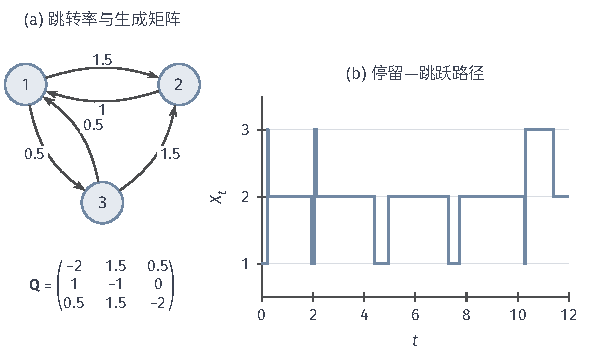
\includegraphics[width=105mm]{figures/03-optimization-evolution-and-signals/02-processes-and-trajectory-evolution/tikz/ctsp-ctmc-path/figure.pdf}
  \caption{三状态连续时间Markov链。(a)箭头上的数是跳转率$q_{i,j}$，生成矩阵的对角元是负的离开率，每行之和为零；(b)从状态$1$出发的一条路径（固定随机种子）：在每个状态停留一段指数时间后跳走，状态$2$只能跳回$1$，离开率最小，因而平均停留最久。}
  \label{fig:ctsp-ctmc-path}
\end{figure}

只看跳跃发生的先后顺序，记$Y_0,Y_1,Y_2,\ldots$为依次访问的状态，就得到一条离散时间Markov链，转移矩阵为$(p_{i,j})$，称为\term{嵌入跳链}（embedded jump chain）。连续时间链等于这条离散链再配上依赖当前状态的指数停留时间。第~\ref{sec:ctsp-occupation}节将看到，两者长期访问各状态的比例可以不同。

\paragraph{矩阵指数与前后向方程}
有限状态时，由构造可以直接验证短时间转移概率：从$i$出发，$h$内不跳的概率为$e^{-q_ih}=1-q_ih+O(h^2)$，恰好跳一次到$j$的概率为$q_{i,j}h+O(h^2)$，跳两次以上的概率为$O(h^2)$。于是$P_h=\bm I+h\bm Q+O(h^2)$，转移概率满足
\begin{equation}
  P_t=e^{t\bm Q},\qquad
  \dot P_t=\bm QP_t\ \text{（后向方程）},\qquad
  \dot P_t=P_t\bm Q\ \text{（前向方程）}.
  \label{eq:ctsp-ctmc-kolmogorov}
\end{equation}
后向方程来自把$[0,t+h]$拆成先走$h$再走$t$，前向方程来自先走$t$再走$h$。若行向量$\bm\mu_t$表示时刻$t$的分布，则$\bm\mu_t=\bm\mu_0P_t$满足$\dot{\bm\mu}_t=\bm\mu_t\bm Q$，逐个分量写出就是
\[
  \frac{\mathrm d}{\mathrm dt}\mu_t(j)=\sum_{i\neq j}\mu_t(i)q_{i,j}-\mu_t(j)q_j ,
\]
即流入$j$的概率流减去流出$j$的概率流。分布不随时间改变当且仅当$\bm\pi\bm Q=\bm0$。

\begin{example}[两态链的转移概率]
  \label{ex:ctsp-two-state}
  取状态$\{1,2\}$，离开$1$的率为$a$，离开$2$的率为$b$，$\bm Q=\begin{pmatrix}-a&a\\b&-b\end{pmatrix}$。$\bm Q$的特征值为$0$和$-(a+b)$，计算矩阵指数得
  \[
    P_t=\frac1{a+b}\begin{pmatrix}b+ae^{-(a+b)t}&a-ae^{-(a+b)t}\\b-be^{-(a+b)t}&a+be^{-(a+b)t}\end{pmatrix}.
  \]
  可以直接核对$P_0=\bm I$与$\dot P_t=\bm QP_t$。$t\to\infty$时两行都趋于$\bm\pi=(b,a)/(a+b)$，且$\bm\pi\bm Q=\bm0$。初值的影响按$e^{-(a+b)t}$消退，速率由$\bm Q$的非零特征值决定。取$a=1,b=2$，得$\bm\pi=(2/3,1/3)$：离开率较小的状态$1$占据更多时间。
\end{example}

\paragraph{可数状态与爆炸}
状态可数无限时，局部速率$\bm Q$还不一定决定一个在所有时刻都有定义的过程。记第$n$次跳跃时刻为$J_n=S_0+\cdots+S_{n-1}$，其中$S_k$是第$k$段停留。若$J_\infty=\lim_nJ_n<\infty$，过程在有限时间内跳了无穷多次，之后的状态没有被构造规定，这称为\term{爆炸}（explosion）。

\begin{example}[纯生过程的爆炸]
  \label{ex:ctsp-explosion}
  在$\{0,1,2,\ldots\}$上只允许$i\to i+1$，离开率$q_i=2^i$。停留时间$S_i\sim\operatorname{Exp}(2^i)$相互独立，$\mathbb EJ_\infty=\sum_i2^{-i}=2<\infty$，所以$J_\infty<\infty$几乎必然：过程在平均两个时间单位内跑遍所有状态。若$q_i=\lambda$为常数，$\mathbb EJ_\infty=\infty$，并且由强大数律$J_n/n\to1/\lambda$，不会爆炸；这正是Poisson计数。
\end{example}

一般地，$J_\infty=\infty$几乎必然当且仅当$\sum_n1/q_{Y_n}=\infty$几乎必然，其中$Y$是嵌入跳链\scite{math-kallenberg2021probability}。由此得到两个常用的充分条件：离开率有界；或嵌入跳链常返，使某个$q_i>0$的状态被访问无穷多次。只给出局部速率时，应当先检查不爆炸，或明确采用在$J_\infty$处停止的“最小过程”；不能把“速率已经给定”等同于“完整过程已经构造好”。

\paragraph{出生死亡链}
很多计数模型只允许状态每次增减一。设状态$k$处的出生率为$\lambda_k$（$k\to k+1$），死亡率为$\mu_k$（$k\to k-1$，$\mu_0=0$），这就是\term{出生死亡链}（birth--death chain）。$\mu_k\equiv0$、$\lambda_k\equiv\lambda$时它退化为Poisson计数；$\lambda_k\equiv\lambda$、$\mu_k\equiv\mu$（$k\geq1$）时，它描述单服务台排队的队长：顾客以速率$\lambda$到来，服务以速率$\mu$完成。

出生死亡链的平衡分布可以由相邻状态之间的概率流平衡求出。在$k$与$k+1$之间，单位时间内从$k$上行的平均次数为$\pi_k\lambda_k$，从$k+1$下行的平均次数为$\pi_{k+1}\mu_{k+1}$。令二者相等，
\begin{equation}
  \pi_k\lambda_k=\pi_{k+1}\mu_{k+1},\qquad
  \pi_k=\pi_0\prod_{j=0}^{k-1}\frac{\lambda_j}{\mu_{j+1}} .
  \label{eq:ctsp-birth-death-balance}
\end{equation}
这是连续时间的细致平衡。对每个$j$，$(\bm\pi\bm Q)_j=\pi_{j-1}\lambda_{j-1}-\pi_j(\lambda_j+\mu_j)+\pi_{j+1}\mu_{j+1}$，把细致平衡的两个等式代入，各项两两抵消，所以它蕴含$\bm\pi\bm Q=\bm0$。排队例中$\pi_k=(1-\rho)\rho^k$，$\rho=\lambda/\mu$，只有$\rho<1$时求和归一化才可能；$\rho\geq1$时队长没有平衡分布，平均意义下会无限增长或零常返地游荡。图~\ref{fig:ctsp-birth-death}画出了$\rho=0.6$的情形。这个模型的速率不超过$\lambda+\mu$，所以不会爆炸。

\begin{figure}[htbp]
  \centering
  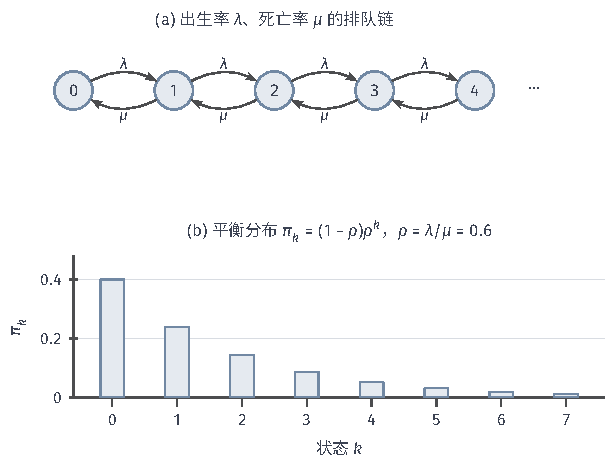
\includegraphics[width=105mm]{figures/03-optimization-evolution-and-signals/02-processes-and-trajectory-evolution/tikz/ctsp-birth-death/figure.pdf}
  \caption{单服务台排队的出生死亡链。(a)上行箭头为到达率$\lambda$，下行箭头为服务率$\mu$，状态$0$不能再下行；(b)$\rho=\lambda/\mu=0.6$时由细致平衡得到的几何平衡分布$\pi_k=(1-\rho)\rho^k$，只画出$k\leq7$。}
  \label{fig:ctsp-birth-death}
\end{figure}

\subsection{停止后的Markov过程}
\label{sec:ctsp-strong-markov}

\paragraph{离散证明为何不能照搬}
第~\ref{chap:discrete-time-stochastic-processes}章证明了离散链的\term{强Markov性质}（strong Markov property）：在停时$\tau$处，给定$\mathcal F_\tau$，过程从$X_\tau$重新开始，后续规律与从该状态出发的链相同。证明把事件按$\{\tau=n\}$分解，在每一块上使用普通Markov性质，再对$n$求和。连续停时可以取不可数多个值，每个取值的概率都可能为零，这种分解失效。本小节用式~\eqref{eq:ctsp-dyadic-stopping}的离散逼近绕过这一困难，并说明为此需要哪些路径和半群条件。

\paragraph{Brownian运动的强Markov性质}
先看最重要的情形。

\begin{theorem}[Brownian运动的强Markov性质]
  \label{thm:ctsp-brownian-strong-markov}
  设$W$是相对于满足通常条件的滤过的标准Brownian运动，$\tau$是停时且$\mathbb P(\tau<\infty)=1$。则$B_t=W_{\tau+t}-W_\tau$，$t\geq0$，是标准Brownian运动，并且独立于$\mathcal F_\tau$。
\end{theorem}

\begin{proof}
固定时刻$0\leq t_1<\cdots<t_m$、有界连续函数$g:\mathbb R^m\to\mathbb R$和$A\in\mathcal F_\tau$，只需证明
\begin{equation}
  \mathbb E[g(B_{t_1},\ldots,B_{t_m})\mathbb I_A]=\mathbb E\,g(W_{t_1},\ldots,W_{t_m})\cdot\mathbb P(A).
  \label{eq:ctsp-strong-markov-target}
\end{equation}
取$\tau_n$如式~\eqref{eq:ctsp-dyadic-stopping}，记$B^{(n)}_t=W_{\tau_n+t}-W_{\tau_n}$。因为$\tau\leq\tau_n$，$A\in\mathcal F_\tau\subseteq\mathcal F_{\tau_n}$，从而$A\cap\{\tau_n=k2^{-n}\}\in\mathcal F_{k2^{-n}}$。在这一块上，$B^{(n)}$就是固定时刻$k2^{-n}$之后的增量过程，独立于$\mathcal F_{k2^{-n}}$并且是标准Brownian运动。对可数个$k$求和，
\[
  \begin{aligned}
    \mathbb E[g(B^{(n)}_{t_1},\ldots,B^{(n)}_{t_m})\mathbb I_A]
    &=\sum_k\mathbb E\,g(W_{t_1},\ldots,W_{t_m})\,\mathbb P(A\cap\{\tau_n=k2^{-n}\})\\
    &=\mathbb E\,g(W_{t_1},\ldots,W_{t_m})\,\mathbb P(A).
  \end{aligned}
\]
令$n\to\infty$。路径连续且$\tau_n\downarrow\tau$，所以$B^{(n)}_{t_i}\to B_{t_i}$逐点成立；$g$有界连续，由控制收敛定理左端趋于式~\eqref{eq:ctsp-strong-markov-target}的左端。有限维分布与独立性因此成立；$B$的路径连续直接继承自$W$。
\end{proof}

证明中两个条件各有分工。停时性质保证$A\cap\{\tau_n=k2^{-n}\}$在时刻$k2^{-n}$已知，从而可以使用固定时刻的独立增量；路径连续保证离散逼近的极限就是停时处的值。对一般Markov过程，第二步需要把$P_tf(X_{\tau_n})$的极限传到$P_tf(X_\tau)$，这要求路径右连续，并且$x\mapsto P_tf(x)$对连续的$f$仍连续。满足后一条件（并在无穷远处保持趋零）的半群称为Feller半群，具有右连续路径的Feller过程都满足强Markov性质\scite{math-kallenberg2021probability}。连续时间Markov链在跳跃时刻重新开始，则直接由停留—跳跃的构造得到。

\paragraph{普通Markov性质不够}
没有路径与半群的正则条件，强Markov性质可能失效。设$\xi\sim\operatorname{Exp}(1)$，令$X_t=(t-\xi)^+$：过程在$0$处停留一段指数时间，然后以单位速度向右移动。由指数分布的无记忆性，它对每个固定时刻都满足Markov性质，转移规则是“在$0$处等待一段$\operatorname{Exp}(1)$时间后离开，在正半轴上匀速右移”。但在右连续滤过下，$\tau=\inf\{t:X_t>0\}=\xi$是停时，$X_\tau=0$，而过程在$\tau$之后立刻离开$0$，不会再等待一段指数时间。从$X_\tau$重新开始的规律与转移核给出的规律不同。问题出在半群的连续性上：对连续的$f$，$x>0$时$P_tf(x)=f(x+t)$，在$x\downarrow0$时趋于$f(t)$，而$P_tf(0)=\mathbb Ef((t-\xi)^+)$一般不等于$f(t)$。$P_tf$在零点不连续，Feller条件不成立，离散逼近的极限步骤因此无法完成。

\paragraph{反射原理}
强Markov性质的价值在于它把“首次到达之后”的路径变成一个新的、可以计算的Brownian运动。设$a>0$，$\tau_a=\inf\{t:W_t=a\}$。由路径连续，$W_{\tau_a}=a$。在$\tau_a$之后，路径向上与向下是对称的：由定理~\ref{thm:ctsp-brownian-strong-markov}，$B_s=W_{\tau_a+s}-a$是独立于$\mathcal F_{\tau_a}$的Brownian运动，与$-B$同分布。于是对$t>0$，
\[
  \mathbb P(W_t\geq a)=\mathbb P(\tau_a\leq t,\ B_{t-\tau_a}\geq0)=\tfrac12\,\mathbb P(\tau_a\leq t),
\]
这里使用了$\tau_a$与$B$独立，以及$B$在任何正时刻取正、负值的概率各为一半（取零的概率为零）。记$M_t=\max_{s\leq t}W_s$，由$\{M_t\geq a\}=\{\tau_a\leq t\}$得到
\begin{equation}
  \mathbb P(M_t\geq a)=2\,\mathbb P(W_t\geq a)=2\bigl[1-\Phi(a/\sqrt t)\bigr],
  \label{eq:ctsp-reflection}
\end{equation}
其中$\Phi$是标准正态分布函数。这一结果称为\term{反射原理}（reflection principle）：把首次到达$a$之后的路径关于水平线$a$翻折，终点在$a$上方与下方的路径一一对应。

式~\eqref{eq:ctsp-reflection}给出两个以后会用到的事实。令$t\to\infty$，$\mathbb P(\tau_a<\infty)=1$：Brownian运动必然到达任意给定高度。对$t$求导得$\tau_a$的密度$a(2\pi t^3)^{-1/2}e^{-a^2/(2t)}$，它按$t^{-3/2}$衰减，所以$\mathbb E\tau_a=\infty$。到达是必然的，平均等待却是无穷的；第~\ref{sec:ctsp-optional-sampling}节将看到，这正是可选抽样在这里失效的原因。

\section{鞅、停止与补偿}
\label{sec:ctsp-martingales}

上一节研究给定当前状态后整个条件未来的分布；本节只看条件均值。第~\ref{chap:discrete-time-stochastic-processes}章的核心问题是：给定历史后，增量还有没有可以预知的平均漂移？没有漂移的累计量是鞅，它在停时处保持期望，最大偏差受终点矩控制，有界时还会收敛。这些结论在连续时间中都成立，但需要补上三类条件：路径要取右连续版本，停时要用离散停时逼近，积分前还常常需要局部化。计数过程还要扣掉“平均会来多少事件”这一可预测部分，才能得到鞅，这就是补偿。

\subsection{连续时间鞅与局部鞅}
\label{sec:ctsp-continuous-martingales}

\paragraph{任意两时刻的条件均值}
离散鞅的定义只比较相邻时刻：$\mathbb E[M_{n+1}\mid\mathcal F_n]=M_n$，再由塔式性质推出任意$m\leq n$的关系。连续时间没有相邻时刻，定义直接要求任意两个时刻。

\begin{definition}[连续时间鞅]
  \label{def:ctsp-martingale}
  适应过程$(M_t)_{t\geq0}$称为相对于$(\mathcal F_t)$的\term{鞅}，若每个$M_t$可积，并且对任意$0\leq s\leq t$，$\mathbb E[M_t\mid\mathcal F_s]=M_s$几乎必然。把等号换成“$\geq$”或“$\leq$”分别得到次鞅与超鞅。
\end{definition}

在满足通常条件的滤过下，每个鞅都有右连续有左极限的修改\scite{math-kallenberg2021probability}，本章总取这样的版本。由引理~\ref{lem:ctsp-right-continuous-modification}，这个版本在不可区分意义下唯一，所以“鞅的路径”是有确切意义的对象。

Brownian运动提供了几个基本的鞅。设$s\leq t$，记$\Delta=W_t-W_s$，它独立于$\mathcal F_s$且服从$\mathcal N(0,t-s)$。
\begin{itemize}
  \item $W_t$：$\mathbb E[W_t\mid\mathcal F_s]=W_s+\mathbb E\Delta=W_s$。
  \item $W_t^2-t$：$\mathbb E[W_t^2\mid\mathcal F_s]=W_s^2+2W_s\mathbb E\Delta+\mathbb E\Delta^2=W_s^2+(t-s)$。
  \item $\exp(\theta W_t-\theta^2t/2)$，$\theta\in\mathbb R$：由$\mathbb Ee^{\theta\Delta}=e^{\theta^2(t-s)/2}$，条件期望恰好抵消多出的指数因子。
\end{itemize}
第二个例子说明，$W_t^2$是次鞅，它的平均增长率正好是$1$；减去$t$以后才没有漂移。这一“减去可预测增长”的操作在计数过程上表现得更加直观。

设$N$是速率$\lambda$的Poisson过程，$\widetilde N_t=N_t-\lambda t$。增量$N_t-N_s$独立于$\mathcal F_s$，均值与方差都是$\lambda(t-s)$，同样的计算给出：$\widetilde N_t$与$\widetilde N_t^2-\lambda t$都是鞅。图~\ref{fig:ctsp-compensated-poisson}比较了扣除平均前后的路径。原始计数整体向上倾斜，补偿后的路径在每个到达时刻仍向上跳一格，在两次到达之间以斜率$-\lambda$下降；路径束围绕零散开，宽度大约按$\sqrt{\lambda t}$增长。

\begin{figure}[htbp]
  \centering
  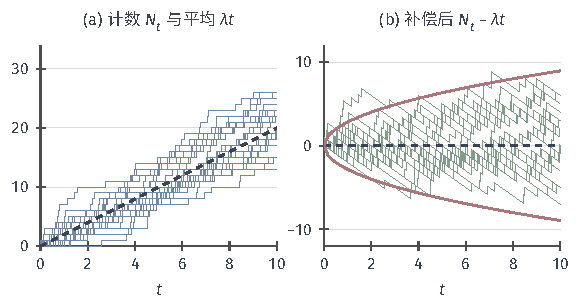
\includegraphics[width=98mm]{figures/03-optimization-evolution-and-signals/02-processes-and-trajectory-evolution/tikz/ctsp-compensated-poisson/figure.pdf}
  \caption{扣除平均累计前后的计数路径。$25$条独立的Poisson路径，速率$\lambda=2$，固定随机种子。(a)原始计数$N_t$围绕平均$\lambda t$（虚线）上升；(b)补偿后的$N_t-\lambda t$在到达时刻仍跳高一格，到达之间按斜率$-2$下降，虚线为零均值，红线为$\pm2\sqrt{\lambda t}$，即两倍标准差的解析曲线，不是置信带。}
  \label{fig:ctsp-compensated-poisson}
\end{figure}

\paragraph{局部化与局部鞅}
后面构造的随机积分$\int_0^tH_s\,\mathrm dW_s$在只知道$\int_0^tH_s^2\,\mathrm ds<\infty$几乎必然时，未必可积，于是不能直接称为鞅。处理办法与离散章的停止过程相同：用一列停时把过程截在“还受控制”的范围内，在每个截断上它是真鞅。

\begin{definition}[局部鞅]
  \label{def:ctsp-local-martingale}
  右连续适应过程$M$称为\term{局部鞅}（local martingale），若存在停时列$\rho_n\uparrow\infty$几乎必然，使每个停止过程$M^{\rho_n}_t=M_{t\wedge\rho_n}$都是鞅。这样的$(\rho_n)$称为\term{局部化}（localization）序列。
\end{definition}

“局部”指的是在随机时间范围内局部，而不是在状态空间中局部。每条路径最终会被某个$\rho_n$覆盖到任意给定的有限时刻，但这并不保证去掉截断后仍可以交换极限与期望。局部鞅不一定是鞅：在三维中，$1/\|\bm W_t+\bm x_0\|$（$\bm x_0\neq\bm0$）是局部鞅，期望却随时间严格下降\scite{math-kallenberg2021probability}。取期望之前，必须另外验证可积性。

有两类情形可以从局部鞅回到鞅或超鞅，后面都会用到。第一，若$\mathbb E\sup_{s\leq t}|M_s|<\infty$对每个$t$成立，控制收敛定理允许在$\mathbb E[M_{t\wedge\rho_n}\mid\mathcal F_s]=M_{s\wedge\rho_n}$中令$n\to\infty$，所以$M$是鞅。第二，非负局部鞅是超鞅：对$s\leq t$，由条件Fatou引理，
\[
  \begin{aligned}
    \mathbb E[M_t\mid\mathcal F_s]&=\mathbb E\bigl[\liminf_nM_{t\wedge\rho_n}\bigm|\mathcal F_s\bigr]\\
    &\leq\liminf_n\mathbb E[M_{t\wedge\rho_n}\mid\mathcal F_s]=\liminf_nM_{s\wedge\rho_n}=M_s .
  \end{aligned}
\]
非负性使Fatou引理可用；可积性也由此得到：$\mathbb EM_t\leq\mathbb EM_0$。这一事实将在第~\ref{sec:ctsp-girsanov}节判断路径权重是否保持总质量，并在第~\ref{sec:ctsp-sa-lyapunov}节构造连续时间的几乎超鞅。

\subsection{可选抽样、最大偏差与极限}
\label{sec:ctsp-optional-sampling}

\paragraph{从离散停时到连续停时}
离散章证明了有界停时的可选抽样：若$\sigma\leq\tau\leq K$，则$\mathbb E[M_\tau\mid\mathcal F_\sigma]=M_\sigma$。连续时间的证明分两步：先对式~\eqref{eq:ctsp-dyadic-stopping}的二进逼近使用离散结论，再借路径右连续和一致可积性取极限。

\begin{theorem}[连续时间的可选抽样]
  \label{thm:ctsp-optional-sampling}
  设$M$是右连续鞅，$\sigma\leq\tau$是停时，且$\tau\leq K$对某个常数$K$成立。则$M_\tau$可积，并且$\mathbb E[M_\tau\mid\mathcal F_\sigma]=M_\sigma$。特别地，$\mathbb EM_\tau=\mathbb EM_0$。
\end{theorem}

\begin{proof}
取$\sigma_n,\tau_n$为$\sigma,\tau$的二进上逼近。它们只取网格$2^{-n}\mathbb N$上的值，并且$\sigma_n\leq\tau_n\leq K+1$。在这一网格上，$(M_{k2^{-n}})_k$是离散鞅，离散可选抽样给出：对$A\in\mathcal F_\sigma\subseteq\mathcal F_{\sigma_n}$，
\[
  \mathbb E[M_{\tau_n}\mathbb I_A]=\mathbb E[M_{\sigma_n}\mathbb I_A].
\]
令$n\to\infty$。右连续性给出$M_{\tau_n}\to M_\tau$与$M_{\sigma_n}\to M_\sigma$逐点成立。离散可选抽样又给出$M_{\tau_n}=\mathbb E[M_{K+1}\mid\mathcal F_{\tau_n}]$，同一可积变量的条件期望族一致可积，所以收敛也在$L^1$中成立，可以在等式两端取极限。于是$\mathbb E[M_\tau\mathbb I_A]=\mathbb E[M_\sigma\mathbb I_A]$对所有$A\in\mathcal F_\sigma$成立，而$M_\sigma$是$\mathcal F_\sigma$可测的（渐进可测过程在停时处的取值可测），结论成立。
\end{proof}

对无界停时，定理给出$\mathbb EM_{\tau\wedge t}=\mathbb EM_0$对每个$t$成立。把$t$送到无穷要交换极限与期望，需要停止过程$(M_{\tau\wedge t})_{t\geq0}$一致可积，或被某个可积变量控制。第~\ref{sec:ctsp-strong-markov}节的首次到达时刻$\tau_a$给出了反例：$\tau_a<\infty$几乎必然且$W_{\tau_a}=a$，但$\mathbb EW_{\tau_a}=a\neq0=\mathbb EW_0$。条件不成立的地方在于停止过程$W_{t\wedge\tau_a}$向下没有界，并且$\mathbb E\tau_a=\infty$。

\paragraph{首次退出的计算}
当停止过程有界时，可选抽样可以直接用来计算。设$a<x<b$，Brownian运动从$x$出发，即考虑$X_t=x+W_t$，令$\tau=\inf\{t:X_t\notin(a,b)\}$为首次退出区间的时刻。下面逐步核对所需条件。

第一，$\tau$是停时：它是连续适应过程首次到达闭集$(-\infty,a]\cup[b,\infty)$的时刻。第二，$\tau$有限且可积。对鞅$X_t^2-t$在有界停时$\tau\wedge t$处使用定理~\ref{thm:ctsp-optional-sampling}，
\[
  \mathbb E(\tau\wedge t)=\mathbb EX_{\tau\wedge t}^2-x^2\leq\max(a^2,b^2),
\]
因为停止前$X$留在$[a,b]$中。令$t\to\infty$，单调收敛定理给出$\mathbb E\tau\leq\max(a^2,b^2)<\infty$。第三，由路径连续，$X_\tau\in\{a,b\}$。

现在对两个鞅取极限。$X_{\tau\wedge t}$取值于$[a,b]$，有界，控制收敛给出$\mathbb EX_\tau=x$。记$p=\mathbb P(X_\tau=b)$，则$pb+(1-p)a=x$，即
\begin{equation}
  \mathbb P_x(X_\tau=b)=\frac{x-a}{b-a}.
  \label{eq:ctsp-exit-probability}
\end{equation}
再对$X_t^2-t$令$t\to\infty$：$X^2_{\tau\wedge t}$有界，$\tau\wedge t$单调上升，两项分别用控制收敛与单调收敛，得到$\mathbb E\tau=\mathbb EX_\tau^2-x^2=pb^2+(1-p)a^2-x^2$。代入$p$并化简，
\begin{equation}
  \mathbb E_x\tau=(x-a)(b-x).
  \label{eq:ctsp-exit-time}
\end{equation}
例如区间$(0,1)$、起点$0.3$时，路径先到达$1$的概率为$0.3$，平均退出时间为$0.21$。第~\ref{sec:ctsp-first-passage}节会把同样的结果解释为边值问题的解。

\paragraph{最大偏差}
很多时候我们关心的不是终点误差，而是整个运行区间上最坏的偏离。离散章的Doob最大不等式控制了$\max_{k\leq n}|M_k|$；连续时间的上确界涉及不可数多个时刻，需要右连续性把它化为可数集上的上确界。

\begin{theorem}[Doob最大不等式]
  \label{thm:ctsp-doob-maximal}
  设$X$是右连续的非负次鞅，$t>0$，$\lambda>0$。则
  \[
    \lambda\,\mathbb P\Bigl(\sup_{s\leq t}X_s>\lambda\Bigr)\leq\mathbb EX_t .
  \]
  若$M$是右连续鞅且$\mathbb EM_t^2<\infty$，则$\mathbb E\sup_{s\leq t}M_s^2\leq4\,\mathbb EM_t^2$。
\end{theorem}

\begin{proof}
令$D_n=\{kt2^{-n}:0\leq k\leq2^n\}$。在有限集$D_n$上，离散Doob不等式给出$\lambda\mathbb P(\max_{s\in D_n}X_s>\lambda)\leq\mathbb EX_t$。$D_n$递增，事件$\{\max_{D_n}X_s>\lambda\}$随$n$上升到$\{\sup_{s\in D}X_s>\lambda\}$，其中$D=\bigcup_nD_n$；由右连续性，$D$上的上确界等于$[0,t]$上的上确界，因为任一时刻的取值都是$D$中从右侧逼近的点的极限。概率的单调连续性完成第一式。第二式同样先在$D_n$上使用离散的$L^2$版本（作用于非负次鞅$|M|$），再由单调收敛取极限。
\end{proof}

例如对Brownian运动，$W_t^2$是非负次鞅，第一式给出$\mathbb P(\sup_{s\leq1}|W_s|\geq3)\leq\mathbb EW_1^2/9=1/9$。由反射原理可以算出精确值至多为$4[1-\Phi(3)]\approx0.0054$，所以这个界很粗糙；它的价值在于只用终点的二阶矩就控制了整个时段，并且对任何平方可积鞅都适用。第~\ref{sec:ctsp-sde-existence}节用第二式控制Picard迭代在整个时段上的误差。

\paragraph{鞅的收敛}
最后看时间趋于无穷时的极限。离散章用上穿次数证明了：$L^1$有界的次鞅几乎必然收敛。连续时间先在可数稠密集上计数上穿，再由右连续性把结论推广到全部时刻。

\begin{theorem}[连续时间鞅收敛]
  \label{thm:ctsp-martingale-convergence}
  设$X$是右连续次鞅，且$\sup_t\mathbb EX_t^+<\infty$。则$X_t$几乎必然收敛到一个可积的极限$X_\infty$。若$M$是一致可积的右连续鞅，则还有$M_t\to M_\infty$于$L^1$，且$M_t=\mathbb E[M_\infty\mid\mathcal F_t]$；若$\sup_t\mathbb EM_t^2<\infty$，则收敛也在$L^2$中成立。
\end{theorem}

三个结论的条件各不相同，不能混用。指数鞅$Z_t=\exp(W_t-t/2)$说明了这一点：它是非负鞅，$\mathbb EZ_t=1$，满足第一个条件，所以几乎必然收敛。由于$W_t/t\to0$几乎必然（对整数时刻用强大数律，再用最大不等式控制相邻整数之间的波动），指数$W_t-t/2\to-\infty$，极限$Z_\infty=0$。期望从$1$跳到$0$，所以$Z$不一致可积，$L^1$收敛不成立。路径有极限，不等于期望也有相同的极限。

\subsection{计数补偿与累计波动}
\label{sec:ctsp-compensation}

\paragraph{常强度计数的补偿}
上一小节已经核验$\widetilde N_t=N_t-\lambda t$是鞅。把这一计算写成一般原则：计数过程$N$本身是次鞅，它的增长可以拆成两部分，一部分是事先就能预期的平均增长$\lambda t$，另一部分是事件实际何时发生带来的随机起伏。前者称为补偿量，后者是鞅。

\begin{theorem}[Poisson补偿]
  \label{thm:ctsp-poisson-compensation}
  设$N$是相对于$(\mathcal F_t)$的速率$\lambda$的Poisson过程。则$\widetilde N_t=N_t-\lambda t$与$\widetilde N_t^2-\lambda t$都是平方可积鞅。
\end{theorem}

\begin{proof}
对$s<t$，$N_t-N_s$独立于$\mathcal F_s$，均值与方差都是$\lambda(t-s)$。第一式由$\mathbb E[\widetilde N_t-\widetilde N_s\mid\mathcal F_s]=0$得到。展开$\widetilde N_t^2=(\widetilde N_s+(\widetilde N_t-\widetilde N_s))^2$，交叉项的条件期望为零，平方项的条件期望为$\lambda(t-s)$，得到第二式。
\end{proof}

\paragraph{可预测强度与补偿量}
事件速率常常随时间或状态改变。门店的顾客在午间更多；连续时间Markov链从状态$i$跳往$j$的速率为$q_{i,j}$，只在链处于$i$时才起作用。设$N$是不爆炸的计数过程，$\lambda_t\geq0$是可预测过程，并且对每个$t$，$\int_0^t\lambda_s\,\mathrm ds<\infty$几乎必然。若
\begin{equation}
  N_t-\int_0^t\lambda_s\,\mathrm ds\quad\text{是局部鞅},
  \label{eq:ctsp-intensity}
\end{equation}
就称$\lambda_t$为$N$的强度，$\Lambda_t=\int_0^t\lambda_s\,\mathrm ds$为\term{补偿量}（compensator）。确定性强度$\lambda(t)$给出非齐次Poisson过程；对连续时间Markov链，从$i$到$j$的跳跃次数$N^{i,j}_t$的强度为$q_{i,j}\mathbb I\{X_{t-}=i\}$。

式~\eqref{eq:ctsp-intensity}中的三个条件各有用途。可预测性要求强度只用严格早于当前时刻的信息，第~\ref{sec:ctsp-time-jump-integrals}节将用一个具体计算说明，若允许强度看到当次事件，零均值性质就会被破坏。不爆炸保证$N_t$有限。累计强度有限则使局部化可行：取$\rho_n=\inf\{t:N_t\geq n\text{ 或 }\Lambda_t\geq n\}$，停止后的计数与补偿量都不超过$n+1$，从而可积，鞅等式可以在每个截断上核对。

\paragraph{三种累计量}
计数过程还带来三个容易混淆的累计量。以常强度Poisson过程为例：原始计数$N_t$记录实际发生了多少事件；补偿后的$\widetilde N_t$是扣除平均增长后的噪声；描述噪声大小的又有两种量。沿路径累计跳跃的平方，得到$[\widetilde N]_t=\sum_{s\leq t}(\Delta\widetilde N_s)^2=N_t$，它是随机的；使$\widetilde N_t^2-\langle\widetilde N\rangle_t$成为鞅的可预测累计量是$\langle\widetilde N\rangle_t=\lambda t$，它是确定的。前者是实现出来的波动，后者是预先可知的波动预算，二者的期望相同。

复合Poisson过程有同样的结构。若$\mathbb E|J_1|<\infty$，$C_t-\lambda t\,\mathbb EJ_1$相对于记录到达时刻与标记的历史是鞅；若再有$\mathbb EJ_1^2<\infty$，平方跳跃累计为$\sum_{k\leq N_t}J_k^2$，可预测二阶累计为$\lambda t\,\mathbb EJ_1^2$，与式~\eqref{eq:ctsp-compound-moments}一致。例如每次理赔恒为$2$时，平均累计速率为$2\lambda$，二阶累计速率却是$4\lambda$。下一节的跳跃积分要把可预测的系数乘到这些补偿增量上，并用可预测二阶累计控制其方差。

更一般地，Doob--Meyer分解断言：满足适当一致可积条件（D类）的右连续次鞅可以唯一地写成鞅与可预测非减过程之和\scite{math-kallenberg2021probability}。计数过程的补偿是它最直观的实例。这一定理不说明任意适应过程都有这样的分解，也不保证分解出的鞅平方可积；本章只在已经核对条件的具体过程上使用补偿。

\section{随机累计与变量变换}
\label{sec:ctsp-stochastic-integration}

离散章的鞅变换$\sum_kH_k(M_{k+1}-M_k)$把每一步开始时选定的权重乘到下一步的噪声上，再累计起来；只要权重不偷看下一步，累计量仍是鞅。本节把这个运算推广到连续时间：给定被积过程$H$和驱动（时间、计数或Brownian运动），定义累计量$\int_0^tH_s\,\mathrm dX_s$，再计算状态函数$f(X_t)$怎样变化。这里被积过程与驱动都是事先给定的；系数依赖未知状态、需要求解的情形留给下一节。

三类驱动的处理方式不同。时间与有限次跳跃可以逐路径累计；Brownian路径的总变差无限，必须借助均方误差在$L^2$中构造积分。变量变换同样分化：有限变差路径遵守普通链式法则，Brownian路径的二次变差留下一个二阶修正，跳跃则保留完整的有限差。

\subsection{时间积分与跳跃积分}
\label{sec:ctsp-time-jump-integrals}

\paragraph{逐路径的时间积分}
最简单的累计是对时间积分。设$b$渐进可测，并且对每个$t$，$\int_0^t|b_s|\,\mathrm ds<\infty$几乎必然。对每条路径，$A_t=\int_0^tb_s\,\mathrm ds$是普通的Lebesgue积分；渐进可测性保证$A_t$是$\mathcal F_t$可测的，于是$A$是连续适应过程。取期望并交换积分次序时，用的是Fubini--Tonelli定理，需要$\mathbb E\int_0^t|b_s|\,\mathrm ds<\infty$；这些积分工具见\BookChapterRef{chap:integration}{卷二“积分”章}。

$A$还具有\term{有限变差}（finite variation）：任一分割上$\sum_i|A_{t_{i+1}}-A_{t_i}|\leq\int_0^t|b_s|\,\mathrm ds$。有限变差的路径可以作为Stieltjes积分的积分器，并且它的平方增量和趋于零，这两点在后面区分不同驱动时都会用到。

\paragraph{计数积分与左极限}
对计数过程$N$，累计只发生在跳跃时刻。对有限值的过程$H$，自然的定义是
\begin{equation}
  \int_0^tH_s\,\mathrm dN_s=\sum_{k:\,T_k\leq t}H_{T_k}.
  \label{eq:ctsp-counting-integral}
\end{equation}
有限时段内只有有限次跳跃，这个和逐路径有定义。问题在于$H$在跳跃时刻取哪个值。若$H$可预测，$H_{T_k}$只依赖$T_k$之前的信息，可以理解为“事件发生前就定好的单次影响”；若$H_s=g(X_{s-})$，取的是跳前状态。

左右极限的差别可以直接算出来。以单位跳跃的计数过程为例，第$k$次事件时$N_{T_k-}=k-1$，$N_{T_k}=k$，于是
\[
  \int_0^tN_{s-}\,\mathrm dN_s=\sum_{k=1}^{N_t}(k-1)=\frac{N_t(N_t-1)}2,\qquad
  \sum_{k=1}^{N_t}N_{T_k}=\frac{N_t(N_t+1)}2 ,
\]
两者相差$N_t$。下面会看到，只有前者与补偿结构相容。

\paragraph{补偿积分的均值与等距}
设$N$是速率$\lambda$的Poisson过程，$H$是可预测过程。扣除平均事件量，定义补偿积分
\begin{equation}
  \int_0^tH_s\,\mathrm d\widetilde N_s=\sum_{k:\,T_k\leq t}H_{T_k}-\lambda\int_0^tH_s\,\mathrm ds .
  \label{eq:ctsp-compensated-integral}
\end{equation}

\begin{theorem}[补偿积分的均值与二阶矩]
  \label{thm:ctsp-poisson-integral}
  设$H$可预测。若\allowbreak$\mathbb E\int_0^T|H_s|\,\mathrm ds<\infty$，则
  \[
    \mathbb E\int_0^TH_s\,\mathrm dN_s=\lambda\,\mathbb E\int_0^TH_s\,\mathrm ds,
  \]
  于是补偿积分的期望为零。若$\mathbb E\int_0^TH_s^2\,\mathrm ds<\infty$，则补偿积分在$[0,T]$上是平方可积鞅，并且
  \begin{equation}
    \mathbb E\Bigl(\int_0^TH_s\,\mathrm d\widetilde N_s\Bigr)^2=\lambda\,\mathbb E\int_0^TH_s^2\,\mathrm ds .
    \label{eq:ctsp-poisson-isometry}
  \end{equation}
\end{theorem}

\begin{proof}
先取简单可预测过程$H_s=\sum_iH_i\mathbb I_{(t_i,t_{i+1}]}(s)$，$H_i$有界且$\mathcal F_{t_i}$可测。此时$\int H\,\mathrm d\widetilde N=\sum_iH_i\Delta\widetilde N_i$，其中$\Delta\widetilde N_i=\widetilde N_{t_{i+1}}-\widetilde N_{t_i}$独立于$\mathcal F_{t_i}$，均值为零，方差为$\lambda\Delta t_i$。每一项的期望$\mathbb E[H_i\,\mathbb E(\Delta\widetilde N_i\mid\mathcal F_{t_i})]=0$；平方展开后，$i<j$的交叉项先对$\mathcal F_{t_j}$取条件期望即为零，对角项给出$\lambda\Delta t_i\,\mathbb EH_i^2$。这证明了简单过程的两个等式，鞅性质由同样的条件期望计算得到。

一般情形用逼近完成。可预测$\sigma$代数由矩形$(s,u]\times A$（$A\in\mathcal F_s$）生成，而矩形指示过程正是简单可预测过程；对可预测集合$B\subseteq(0,T]\times\Omega$，两个有限测度$B\mapsto\mathbb E\int\mathbb I_B\,\mathrm dN$与$B\mapsto\lambda\mathbb E\int\mathbb I_B\,\mathrm ds$在矩形上相等，矩形族对有限交封闭，由单调类定理它们在整个可预测$\sigma$代数上相等。再用简单函数逼近非负可预测$H$并取单调极限，得到第一式；有符号情形对正负部分别使用。二阶等式先对简单过程成立，再按等距在$L^2$中延拓，延拓结果与式~\eqref{eq:ctsp-compensated-integral}的逐路径定义一致，因为第一式保证了两者之差的期望绝对值为零。
\end{proof}

可预测性不是技术细节。若把跳后的$N_s$当作系数，
\[
  \begin{aligned}
    \mathbb E\sum_{k\leq N_t}N_{T_k}&=\mathbb E\frac{N_t(N_t+1)}2=\frac{(\lambda t)^2}2+\lambda t,\\
    \lambda\,\mathbb E\int_0^tN_s\,\mathrm ds&=\lambda\int_0^t\lambda s\,\mathrm ds=\frac{(\lambda t)^2}2,
  \end{aligned}
\]
两者之差为$\lambda t\neq0$：声称的“补偿积分”有正的平均漂移。原因是跳后的系数在事件发生的那一刻把这次事件也算了进去。改用$N_{s-}$，$\mathbb EN_t(N_t-1)/2=(\lambda t)^2/2$，差恰好消失。

若只知道每个有限$T$上$\int_0^TH_s^2\,\mathrm ds<\infty$几乎必然，可以取停时$\rho_n=\inf\{t:\lambda\int_0^tH_s^2\,\mathrm ds\geq n\}\wedge n$。累计平方连续、适应且非减，所以$\rho_n$是停时；停止后的被积过程满足定理的二阶条件，补偿积分因而是局部鞅。去掉截断后能否取零均值，仍需另行检查可积性。

\begin{example}[按跳前状态计费]
  \label{ex:ctsp-predictable-fee}
  一台设备在每次故障时产生维修费用，费用等于故障前已累计的故障次数加一，即$H_s=N_{s-}+1$。$[0,t]$上的总费用为$\int_0^t(N_{s-}+1)\,\mathrm dN_s=N_t(N_t+1)/2$，其期望由定理~\ref{thm:ctsp-poisson-integral}给出：$\lambda\int_0^t(\lambda s+1)\,\mathrm ds=(\lambda t)^2/2+\lambda t$。直接用$\mathbb EN_t^2=(\lambda t)^2+\lambda t$计算，结果相同。这里系数可以依赖全部过去，只要不依赖当次事件。
\end{example}

\subsection{Brownian积分}
\label{sec:ctsp-brownian-integral}

\paragraph{简单可预测过程的累计}
现在把驱动换成Brownian运动。第~\ref{sec:ctsp-brownian}节说明它的路径总变差无限，不能逐路径地定义Stieltjes积分；但离散鞅变换提示了另一条路：先对在有限个时刻改变取值的被积过程定义累计，再利用均方误差把定义推广出去。

设$0=t_0<t_1<\cdots<t_n=T$，$H_i\in L^2(\mathcal F_{t_i})$，称$H_s=\sum_iH_i\mathbb I_{(t_i,t_{i+1}]}(s)$为简单可预测过程。系数在每段开始时确定，可以依赖开始以前的全部历史，但不能借用本段的Brownian增量。定义
\begin{equation}
  \int_0^tH_s\,\mathrm dW_s=\sum_iH_i\bigl(W_{t\wedge t_{i+1}}-W_{t\wedge t_i}\bigr).
  \label{eq:ctsp-simple-ito}
\end{equation}

\begin{lemma}[简单过程的Itô等距]
  \label{lem:ctsp-simple-isometry}
  对简单可预测过程$H$，$M_t=\int_0^tH_s\,\mathrm dW_s$是连续的平方可积鞅，并且
  \[
    \mathbb E\Bigl(\int_0^TH_s\,\mathrm dW_s\Bigr)^2=\mathbb E\int_0^TH_s^2\,\mathrm ds .
  \]
\end{lemma}

\begin{proof}
路径连续由$W$的连续性直接得到。对$s<t$，起点不早于$s$的每一段都满足$\mathbb E[H_i\Delta W_i\mid\mathcal F_s]=\mathbb E\{H_i\,\mathbb E[\Delta W_i\mid\mathcal F_{t_i}]\mid\mathcal F_s\}=0$，包含$s$的那一段用已知系数乘以$s$之后的零均值增量，同样没有条件漂移，所以$M$是鞅。平方展开时，对$i<j$，$H_iH_j\Delta W_i$是$\mathcal F_{t_j}$可测的，而$\Delta W_j$独立于$\mathcal F_{t_j}$且均值为零，交叉项期望为零；对角项为$\mathbb E[H_i^2\,\mathbb E((\Delta W_i)^2\mid\mathcal F_{t_i})]=\Delta t_i\,\mathbb EH_i^2$。逐项相加即得等距。交叉乘积的可积性由Cauchy--Schwarz不等式保证。
\end{proof}

\paragraph{$L^2$延拓}
等距说明，积分把被积过程空间中的距离原样搬到随机变量空间中。记$\mathcal H^2_T$为满足$\mathbb E\int_0^TH_s^2\,\mathrm ds<\infty$的可预测过程全体（几乎处处相等者视为同一元素），范数为$\|H\|^2_{\mathcal H^2}=\mathbb E\int_0^TH_s^2\,\mathrm ds$。它是$[0,T]\times\Omega$上关于测度$\mathrm ds\otimes\mathbb P$、限制在可预测$\sigma$代数上的$L^2$空间，因而是完备的Hilbert空间；$L^2$空间完备性的证明见\BookChapterRef{chap:function-spaces}{卷二“函数空间”章}。简单可预测过程在$\mathcal H^2_T$中稠密\scite{math-oksendal2003sde}：对连续有界的适应过程，取左端点的阶梯逼近，由路径连续与控制收敛即在该范数下收敛；一般情形再由连续过程逼近。

\begin{theorem}[Itô积分]
  \label{thm:ctsp-ito-integral}
  对$H\in\mathcal H^2_T$，取简单可预测过程$H^{(n)}\to H$于$\mathcal H^2_T$。则$\int_0^TH^{(n)}_s\,\mathrm dW_s$在$L^2(\mathbb P)$中收敛，极限不依赖逼近列的选择，记为$\int_0^TH_s\,\mathrm dW_s$，称为\term{Itô积分}（Itô integral）。作为$t\in[0,T]$的函数，它有连续版本，是平方可积鞅，并满足\term{Itô等距}
  \begin{equation}
    \mathbb E\Bigl(\int_0^TH_s\,\mathrm dW_s\Bigr)^2=\mathbb E\int_0^TH_s^2\,\mathrm ds .
    \label{eq:ctsp-ito-isometry}
  \end{equation}
\end{theorem}

\begin{proof}
由引理~\ref{lem:ctsp-simple-isometry}，$\|\int H^{(n)}\mathrm dW-\int H^{(m)}\mathrm dW\|_{L^2}=\|H^{(n)}-H^{(m)}\|_{\mathcal H^2}$，所以积分列是$L^2$中的Cauchy列，由完备性收敛；两列逼近交错排列仍是Cauchy列，极限唯一。等距在极限中保持。条件期望是$L^2$上的压缩，鞅等式在极限中保持。对连续版本，把Doob的$L^2$最大不等式用于差$\int H^{(n)}\mathrm dW-\int H^{(m)}\mathrm dW$，得到$\mathbb E\sup_{t\leq T}|\cdot|^2\leq4\|H^{(n)}-H^{(m)}\|^2_{\mathcal H^2}$；选子列使这些量可求和，Borel--Cantelli引理给出几乎必然的一致收敛，连续函数的一致极限仍连续。
\end{proof}

若只有$\int_0^TH_s^2\,\mathrm ds<\infty$几乎必然，令$\rho_n=\inf\{t:\int_0^tH_s^2\,\mathrm ds\geq n\}\wedge T$。停止后的被积过程属于$\mathcal H^2_T$，各截断上的积分在共同时段上一致，拼接成一个连续的局部鞅。本章说$\int H\,\mathrm dW$时，默认被积过程满足这一局部条件。

\paragraph{两个直接计算}
确定性被积函数给出最简单的例子。若$f$是$[0,T]$上的平方可积确定函数，简单逼近的每一项都是独立高斯增量的线性组合，$L^2$极限仍是高斯变量，所以
\[
  \int_0^Tf(s)\,\mathrm dW_s\sim\mathcal N\Bigl(0,\int_0^Tf(s)^2\,\mathrm ds\Bigr).
\]
这一结论将用于线性随机微分方程的解。

被积过程是Brownian运动本身时，左端点取样的Riemann和可以直接求极限。由恒等式$W_{t_i}\Delta W_i=\frac12[W_{t_{i+1}}^2-W_{t_i}^2-(\Delta W_i)^2]$，
\[
  \sum_iW_{t_i}\Delta W_i=\frac12W_T^2-\frac12\sum_i(\Delta W_i)^2\longrightarrow\frac12(W_T^2-T)\qquad\text{于 }L^2,
\]
最后一步用了定理~\ref{thm:ctsp-brownian-qv}。于是
\begin{equation}
  \int_0^TW_s\,\mathrm dW_s=\frac12(W_T^2-T).
  \label{eq:ctsp-int-w-dw}
\end{equation}
普通微积分会给出$\frac12W_T^2$，多出来的$-\frac T2$就是二次变差留下的痕迹。作为核对，等距给出方差$\int_0^T\mathbb EW_s^2\,\mathrm ds=T^2/2$，而$\operatorname{Var}((W_T^2-T)/2)=\operatorname{Var}(W_T^2)/4=T^2/2$，二者一致。

\paragraph{Itô过程}
把时间积分与Brownian积分合在一起，就得到后面换元公式和随机微分方程的基本对象。

\begin{definition}[Itô过程]
  \label{def:ctsp-ito-process}
  设$\bm W$是$m$维标准Brownian运动，$\bm X_0$是$\mathcal F_0$可测的$\mathbb R^d$值随机向量，$\bm b_t\in\mathbb R^d$渐进可测，$\bm\sigma_t\in\mathbb R^{d\times m}$可预测，并且每个有限$T$上$\int_0^T(\|\bm b_t\|_2+\|\bm\sigma_t\|_{\mathrm F}^2)\,\mathrm dt<\infty$几乎必然。称
  \[
    \bm X_t=\bm X_0+\int_0^t\bm b_s\,\mathrm ds+\int_0^t\bm\sigma_s\,\mathrm d\bm W_s
  \]
  为\term{Itô过程}（Itô process），记作$\mathrm d\bm X_t=\bm b_t\,\mathrm dt+\bm\sigma_t\,\mathrm d\bm W_t$。$\bm b$称为漂移，$\bm\sigma$称为扩散系数；向量积分逐分量理解，$(\int\bm\sigma\,\mathrm d\bm W)_i=\sum_j\int\sigma_{i,j}\,\mathrm dW^{(j)}$。
\end{definition}

记号$\mathrm d\bm X_t$只是积分方程的简写，并不断言$\bm X$可微。Itô过程是有限变差的漂移部分与连续局部鞅之和；这种分解是唯一的，因为一个既是有限变差又是连续局部鞅的过程只能是常数\scite{math-kallenberg2021probability}。

\subsection{二次变差与Itô公式}
\label{sec:ctsp-ito-formula}

\paragraph{从离散平方恒等式出发}
要计算状态函数$f(X_t)$的变化，先回到一条分割上的Taylor展开：
\[
  f(X_t)-f(X_0)=\sum_if'(X_{t_i})\Delta X_i+\frac12\sum_if''(\xi_i)(\Delta X_i)^2 ,
\]
其中$\xi_i$介于$X_{t_i}$与$X_{t_{i+1}}$之间。若$X$是光滑或有限变差的路径，第二个和被$\max_i|\Delta X_i|\cdot\sum_i|\Delta X_i|$控制，趋于零，留下的就是普通链式法则。若$X=W$，平方增量和不消失，第二个和趋于$\frac12\int_0^tf''(W_s)\,\mathrm ds$。这正是Itô公式中二阶修正项的来源。

一般Itô过程的平方增量和需要保留扩散系数。沿网格宽度趋零的分割，
\begin{equation}
  [X^{(i)},X^{(j)}]_t=\lim\sum_k\Delta X^{(i)}_k\Delta X^{(j)}_k=\int_0^t(\bm\sigma_s\bm\sigma_s^\top)_{i,j}\,\mathrm ds\qquad\text{依概率},
  \label{eq:ctsp-ito-covariation}
\end{equation}
称为\term{二次协变差}（quadratic covariation）。漂移部分有限变差，不贡献二次变差；独立Brownian分量的交叉乘积和趋于零，相同分量的平方和趋于时间长度。例如$X=2W$时$[X]_t=4t$，不是$t$。一个有用的形式记忆规则是
\[
  \mathrm dt\cdot\mathrm dt=0,\qquad\mathrm dt\cdot\mathrm dW^{(j)}=0,\qquad\mathrm dW^{(i)}\cdot\mathrm dW^{(j)}=\delta_{i,j}\,\mathrm dt,
\]
它概括的是上述累计量的阶，不能替代可预测性与极限论证。

\paragraph{Itô公式}
下面的定理同时允许被变换的函数显含时间。记$C^{2,1}(\mathbb R^d\times[0,\infty))$为对状态变量二阶、对时间变量一阶连续可微的函数$V(t,\bm x)$全体，即$\partial_tV$、$\nabla V$、$\nabla^2V$都存在且关于$(t,\bm x)$连续。

\begin{theorem}[Itô公式]
  \label{thm:ctsp-ito-formula}
  设$\bm X$是定义~\ref{def:ctsp-ito-process}中的Itô过程，$V\in C^{2,1}(\mathbb R^d\times[0,\infty))$。则存在概率为一的事件，在其上对所有$t\geq0$同时有
  \begin{equation}
    \begin{aligned}
      V(t,\bm X_t)-V(0,\bm X_0)
      ={}&\int_0^t\Bigl[\partial_sV+\nabla V^\top\bm b_s+\tfrac12\operatorname{tr}\bigl(\bm\sigma_s\bm\sigma_s^\top\nabla^2V\bigr)\Bigr]\,\mathrm ds\\
      &+\int_0^t\nabla V^\top\bm\sigma_s\,\mathrm d\bm W_s ,
    \end{aligned}
    \label{eq:ctsp-ito-formula}
  \end{equation}
  其中$\partial_sV,\nabla V,\nabla^2V$都在$(s,\bm X_s)$处取值。微分记号写作
  \[
    \mathrm dV(t,\bm X_t)=\Bigl[\partial_tV+\nabla V^\top\bm b_t+\tfrac12\operatorname{tr}(\bm\sigma_t\bm\sigma_t^\top\nabla^2V)\Bigr]\mathrm dt+\nabla V^\top\bm\sigma_t\,\mathrm d\bm W_t .
  \]
\end{theorem}

式~\eqref{eq:ctsp-ito-formula}称为\term{Itô公式}（Itô formula）。公式的右端分成两部分：时间积分是$V(t,\bm X_t)$的漂移，它比普通链式法则多出$\frac12\operatorname{tr}(\bm\sigma\bm\sigma^\top\nabla^2V)$；随机积分是局部鞅。公式本身逐路径成立，但对它取期望时，随机积分项只是局部鞅，期望为零还需要额外条件，例如$\mathbb E\int_0^t\|\bm\sigma_s^\top\nabla V(s,\bm X_s)\|_2^2\,\mathrm ds<\infty$。

\paragraph{为什么二阶项留下而其余高阶项消失}
完整证明见Øksendal的随机微分方程教材第4章\scite{math-oksendal2003sde}。这里说明各项的去向，以免把二阶修正当作需要死记的规则。先用停时把$\bm X$截在有界区域内、并使系数有界，再在分割上对$V$作Taylor展开到时间一阶、空间二阶。

对时间与空间的一阶项，左端点取值的和分别收敛到$\int\partial_sV\,\mathrm ds$、$\int\nabla V^\top\bm b\,\mathrm ds$与随机积分$\int\nabla V^\top\bm\sigma\,\mathrm d\bm W$；后者正是Itô积分的定义方式，冻结左端点的误差由Itô等距控制。二阶项中，漂移与漂移、漂移与噪声的乘积和分别是$O(|\pi|)$与$O(|\pi|^{1/2})$量级，趋于零；噪声与噪声的乘积和则趋于二次协变差。关键估计是：对有界的$\mathcal F_{t_i}$可测权重$c_i$，
\[
  \mathbb E\Bigl|\sum_ic_i\bigl[(\Delta W_i)^2-\Delta t_i\bigr]\Bigr|^2=2\sum_i\mathbb E[c_i^2](\Delta t_i)^2\leq2\max_i\|c_i\|_\infty^2\,T|\pi| ,
\]
因为不同$i$的项在条件期望下正交，每一项的条件方差为$2(\Delta t_i)^2$。所以加权平方增量和收敛到加权时间积分，而不是零。三阶以上的余项被$\omega(\max_i\|\Delta\bm X_i\|)\sum_i\|\Delta\bm X_i\|^2$控制，其中$\omega$是二阶导数在紧集上的连续模，路径连续使第一个因子趋零，第二个因子依概率有界。最后令停时递增，去掉截断。

\paragraph{计算示例}
几个计算展示公式的用法，每一个都可以与已有结论核对。
\begin{enumerate}
  \item 取$V(x)=x^2$、$X=W$：$\mathrm d(W_t^2)=2W_t\,\mathrm dW_t+\mathrm dt$，积分即得式~\eqref{eq:ctsp-int-w-dw}。
  \item 取$V(x)=x^4$、$X=W$：$\mathrm d(W_t^4)=4W_t^3\,\mathrm dW_t+6W_t^2\,\mathrm dt$。被积过程$4W^3$满足$\mathbb E\int_0^t16W_s^6\,\mathrm ds<\infty$，随机积分是真鞅，取期望得$\mathbb EW_t^4=6\int_0^ts\,\mathrm ds=3t^2$，与正态四阶矩一致。
  \item 取含时间的$V(t,x)=\exp(\theta x-\theta^2t/2)$、$X=W$：$\partial_tV+\frac12\partial_{xx}V=(-\frac{\theta^2}2+\frac{\theta^2}2)V=0$，所以$\mathrm dV(t,W_t)=\theta V(t,W_t)\,\mathrm dW_t$，漂移恰好消失。这从另一角度说明了第~\ref{sec:ctsp-continuous-martingales}节的指数鞅为什么需要因子$e^{-\theta^2t/2}$。
\end{enumerate}

两个Itô过程的乘积是另一个常用特例。对$V(x,y)=xy$使用二维公式，$\nabla^2V$只有非对角元$1$，得到
\begin{equation}
  \mathrm d(X_tY_t)=X_t\,\mathrm dY_t+Y_t\,\mathrm dX_t+\mathrm d[X,Y]_t .
  \label{eq:ctsp-product-rule}
\end{equation}
若其中一个因子有限变差（例如确定函数$e^{\lambda t}$），交叉变差为零，乘积法则与普通微积分相同。下一节求解线性方程时，正是利用这一点构造积分因子。

\paragraph{有限活动跳跃的Itô公式}
最后加入计数驱动。设
\[
  \bm X_t=\bm X_0+\int_0^t\bm b_s\,\mathrm ds+\int_0^t\bm\sigma_s\,\mathrm d\bm W_s+\int_0^t\bm\gamma_s\,\mathrm dN_s ,
\]
其中$N$是速率$\lambda$的Poisson过程，$\bm\gamma$可预测且有限。路径在相邻事件之间是连续Itô过程，在事件时刻$T_k$跳$\Delta\bm X_{T_k}=\bm\gamma_{T_k}$。在相邻事件之间使用定理~\ref{thm:ctsp-ito-formula}，在每个事件处加上$V$的精确增量，再把有限个片段首尾相接，得到：对$V\in C^{2,1}$，
\begin{equation}
  \begin{aligned}
    V(t,\bm X_t)-V(0,\bm X_0)
    ={}&\int_0^t\Bigl[\partial_sV+\nabla V^\top\bm b_s+\tfrac12\operatorname{tr}(\bm\sigma_s\bm\sigma_s^\top\nabla^2V)\Bigr](s,\bm X_{s-})\,\mathrm ds\\
    &+\int_0^t\nabla V(s,\bm X_{s-})^\top\bm\sigma_s\,\mathrm d\bm W_s\\
    &+\int_0^t\bigl[V(s,\bm X_{s-}+\bm\gamma_s)-V(s,\bm X_{s-})\bigr]\,\mathrm dN_s .
  \end{aligned}
  \label{eq:ctsp-jump-ito}
\end{equation}
跳跃项保留的是完整的有限差$V(\bm x+\bm\gamma)-V(\bm x)$，而不是Taylor展开到二阶的近似；跳幅不必很小，推导也不需要它很小。把最后一项写成补偿形式，$\mathrm dN_s=\mathrm d\widetilde N_s+\lambda\,\mathrm ds$，漂移中就多出$\lambda[V(s,\bm X_{s-}+\bm\gamma_s)-V(s,\bm X_{s-})]$，其余部分是零均值的跳跃鞅项（在相应可积条件下）。

\begin{example}[计数平方的修正]
  \label{ex:ctsp-poisson-square}
  取$X=N$、$V(x)=x^2$。每次事件使平方增加$(N_{s-}+1)^2-N_{s-}^2=2N_{s-}+1$，所以$N_t^2=\int_0^t(2N_{s-}+1)\,\mathrm dN_s$。由定理~\ref{thm:ctsp-poisson-integral}，$\mathbb EN_t^2=\lambda\int_0^t(2\lambda s+1)\,\mathrm ds=(\lambda t)^2+\lambda t$，与Poisson分布的二阶矩一致。Brownian平方的修正是连续的$t$，计数平方的修正是随机的事件数$N_t$；后者的平均才是$\lambda t$。
\end{example}

\subsection{Stratonovich积分与普通链式法则}
\label{sec:ctsp-stratonovich}

\paragraph{取样点改变积分}
对有限变差的积分器，Riemann--Stieltjes和取分割中哪一点的被积函数值都不影响极限。Brownian积分不是这样。仍考虑$\int_0^1W\,\mathrm dW$，把左端点换成右端点，两个和之差恰为$\sum_i(\Delta W_i)^2\to1$；换成中点$W_{(t_i+t_{i+1})/2}$，极限则是$\frac12W_1^2$。图~\ref{fig:ctsp-ito-stratonovich-sums}在同一条路径上比较了三种取样：分割加细时，三条折线分别稳定在三个不同的水平上，差值不随网格变细而消失。

\begin{figure}[htbp]
  \centering
  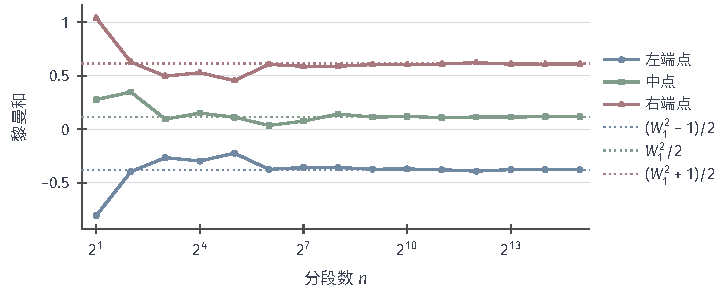
\includegraphics[width=105mm]{figures/03-optimization-evolution-and-signals/02-processes-and-trajectory-evolution/tikz/ctsp-ito-stratonovich-sums/figure.pdf}
  \caption{同一条Brownian教学路径（$2^{16}$个增量，固定随机种子）上$\int_0^1W\,\mathrm dW$的三种Riemann和，横轴为二进分割的段数。左端点、中点、右端点取样分别趋向$(W_1^2-1)/2$、$W_1^2/2$与$(W_1^2+1)/2$（同色点线）。左端点对应Itô积分，中点对应Stratonovich积分；两者之差是二次变差的一半，并非网格误差。}
  \label{fig:ctsp-ito-stratonovich-sums}
\end{figure}

左端点取样的优点是被积系数不偷看本段增量，从而保留鞅性质与等距；代价是普通链式法则需要修正。中点或两端平均取样恢复了普通链式法则，但失去了鞅性质：$\mathbb E\frac12W_1^2=\frac12\neq0$。两种约定各有用途，关键是在建模时说清用的是哪一种。

\paragraph{连续半鞅上的Stratonovich积分}
把有限变差部分与连续局部鞅之和称为\term{连续半鞅}（continuous semimartingale）；Itô过程都是连续半鞅。对连续半鞅$H$与$X$，定义
\begin{equation}
  \int_0^tH_s\circ\mathrm dX_s=\int_0^tH_s\,\mathrm dX_s+\frac12[H,X]_t ,
  \label{eq:ctsp-stratonovich}
\end{equation}
称为\term{Stratonovich积分}（Stratonovich integral）。它是两端平均取样$\sum_i\frac12(H_{t_i}+H_{t_{i+1}})\Delta X_i$的依概率极限：与左端点和相比，多出的$\frac12\sum_i\Delta H_i\Delta X_i$正收敛到$\frac12[H,X]_t$。

普通链式法则在这一约定下恢复。设$F\in C^3$，由Itô公式，
\[
  F(X_t)-F(X_0)=\int_0^tF'(X_s)\,\mathrm dX_s+\frac12\int_0^tF''(X_s)\,\mathrm d[X]_s .
\]
另一方面，$F'(X)$本身是连续半鞅，其鞅部分为$\int F''(X)\,\mathrm dM$（$M$是$X$的鞅部分），所以$[F'(X),X]_t=\int_0^tF''(X_s)\,\mathrm d[X]_s$。代入式~\eqref{eq:ctsp-stratonovich}，得到$F(X_t)-F(X_0)=\int_0^tF'(X_s)\circ\mathrm dX_s$，与普通微积分形式相同。需要$C^3$是为了让$F'(X)$可以再用一次Itô公式。

\paragraph{同一模型的两种写法}
Stratonovich记号写出的方程可以改写为Itô方程，但漂移必须修正。对标量模型$\mathrm dX_t=b_{\mathrm S}(X_t)\,\mathrm dt+\sigma(X_t)\circ\mathrm dW_t$，其中$\sigma\in C^2$，由定义有$\sigma(X)\circ\mathrm dW=\sigma(X)\,\mathrm dW+\frac12\mathrm d[\sigma(X),W]$，而$[\sigma(X),W]_t=\int_0^t\sigma'(X_s)\sigma(X_s)\,\mathrm ds$。于是它等价于
\begin{equation}
  \mathrm dX_t=\Bigl[b_{\mathrm S}(X_t)+\tfrac12\sigma(X_t)\sigma'(X_t)\Bigr]\mathrm dt+\sigma(X_t)\,\mathrm dW_t .
  \label{eq:ctsp-strat-to-ito}
\end{equation}
多维时，第$i$个分量的修正为$\frac12\sum_{j,k}\sigma_{k,j}\partial_k\sigma_{i,j}$。加性噪声（$\sigma$为常数）时修正为零，两种写法给出同一个方程。

\begin{example}[乘性噪声的两种解读]
  \label{ex:ctsp-multiplicative-two-readings}
  考虑$\mathrm dX=aX\,\mathrm dt+\sigma X\circ\mathrm dW$，$X_0=x_0>0$。按Stratonovich约定，普通链式法则可用于$\log X$：$\mathrm d\log X=a\,\mathrm dt+\sigma\circ\mathrm dW$，所以$X_t=x_0\exp(at+\sigma W_t)$，路径的平均指数增长率为$a$。由式~\eqref{eq:ctsp-strat-to-ito}，它等价于Itô方程$\mathrm dX=(a+\sigma^2/2)X\,\mathrm dt+\sigma X\,\mathrm dW$。反过来，若把同样的符号理解为Itô方程$\mathrm dX=aX\,\mathrm dt+\sigma X\,\mathrm dW$，下一节将算出$X_t=x_0\exp((a-\sigma^2/2)t+\sigma W_t)$，增长率变为$a-\sigma^2/2$。取$a=0.05$、$\sigma=0.4$，一个模型的典型路径以$0.05$的速率增长，另一个以$0.03$的速率衰减。两种约定之间的转换保持的是同一个随机模型，单纯更换积分记号而不修改漂移，会把模型换成另一个。
\end{example}

哪种约定更适合建模，取决于噪声的来源。若真实的扰动是相关时间很短的光滑噪声，用它驱动普通微分方程，再让相关时间趋零，在适当条件下极限是Stratonovich方程（Wong--Zakai型结果）\scite{math-oksendal2003sde}；若噪声来自离散时刻独立的冲击，而系数在冲击前确定，Itô约定更自然。有跳跃时，对称取样的约定还要另行规定跳跃处的取值，本章不进入这一情形。

\section{随机微分方程的解}
\label{sec:ctsp-sde}

上一节的被积过程都是事先给定的。现在回到本章开头的第三台记录仪：温度受持续扰动，扰动的强度和温度的回落速度都取决于温度本身。这时漂移与扩散系数是未知状态的函数，累计规则与未知路径互相决定，问题变成求解随机微分方程。本节先说明方程究竟要求什么，再给出解存在唯一的条件，接着计算几个可以显式求解的模型，最后加入跳跃驱动。

\subsection{随机初值问题与解的含义}
\label{sec:ctsp-sde-meaning}

\paragraph{从记号还原为积分方程}
设漂移$\bm b:[0,\infty)\times\mathbb R^d\to\mathbb R^d$与扩散系数$\bm\sigma:[0,\infty)\times\mathbb R^d\to\mathbb R^{d\times m}$是联合Borel可测的函数。\term{随机微分方程}
\begin{equation}
  \mathrm d\bm X_t=\bm b(t,\bm X_t)\,\mathrm dt+\bm\sigma(t,\bm X_t)\,\mathrm d\bm W_t,\qquad\bm X_0=\bm\xi
  \label{eq:ctsp-sde}
\end{equation}
的含义是积分方程
\begin{equation}
  \bm X_t=\bm\xi+\int_0^t\bm b(s,\bm X_s)\,\mathrm ds+\int_0^t\bm\sigma(s,\bm X_s)\,\mathrm d\bm W_s\qquad\text{对所有 }t\geq0,\ \text{几乎必然}.
  \label{eq:ctsp-sde-integral}
\end{equation}
要让右端有意义，必须先固定一组对象：概率空间与满足通常条件的滤过，相对于该滤过的$m$维Brownian运动$\bm W$，以及$\mathcal F_0$可测的初值$\bm\xi$。解是一个连续适应过程$\bm X$，使$\int_0^t(\|\bm b(s,\bm X_s)\|_2+\|\bm\sigma(s,\bm X_s)\|_{\mathrm F}^2)\,\mathrm ds<\infty$几乎必然，并且式~\eqref{eq:ctsp-sde-integral}成立。

与第~\ref{chap:ordinary-differential-equations}章的常微分方程初值问题相比，这里的“解”是一个随机过程：每一条Brownian路径产生一条状态路径，同一个初值在不同噪声下走向不同的轨迹，所有轨迹的分布才是模型的完整输出。若$\bm\sigma\equiv\bm0$，方程退化为逐路径的常微分方程。

\paragraph{强解与弱解}
求解的要求有强弱两种。给定上述全部对象，若能找到满足方程的过程$\bm X$，并且它适应于由初值与驱动$\bm W$生成（并完备化）的滤过，就称为\term{强解}。强解意味着状态路径是“初值与噪声路径的一个函数”，不需要额外的随机来源。若只要求存在某个概率空间、其上的Brownian运动与过程，使方程成立且初值分布符合要求，就称为\term{弱解}（weak solution）；这时驱动本身也是求解的一部分。

唯一性也分两种。\term{路径唯一性}（pathwise uniqueness）比较同一空间、同一初值、同一驱动上的两个解，要求它们不可区分；\term{分布唯一性}（uniqueness in law）只要求任意两个弱解的路径分布相同。一个经典例子说明这些概念确实不同：方程$\mathrm dX_t=\operatorname{sgn}(X_t)\,\mathrm dW_t$，$X_0=0$（约定$\operatorname{sgn}(0)=-1$）有弱解，并且分布唯一（任何解都是Brownian运动），但若$X$是解，$-X$在几乎所有时刻也满足同一方程，路径唯一性失败，并且它没有强解\scite{math-kallenberg2021probability}。反过来，Yamada--Watanabe定理说明，弱解存在加上路径唯一性就推出强解存在与分布唯一。

这里的“强”与“弱”只关于解的构造方式。第~\ref{sec:ctsp-numerical}节的数值强误差、弱误差比较的是数值近似与真解，属于另一组概念，二者不应混用。

\subsection{存在、唯一与依赖关系}
\label{sec:ctsp-sde-existence}

\paragraph{全局Lipschitz条件下的Picard迭代}
常微分方程的存在唯一定理用Picard迭代：把候选轨迹代入右端积分，得到新的候选，在适当的范数下这是压缩映射。随机方程沿用同一思路，只是距离要换成能同时控制整个时段的均方距离；需要新增的两件工具，一是Itô等距控制随机积分的二阶矩，二是Doob最大不等式把终点的控制扩展到整个时段。

先回顾一个工具。第~\ref{chap:ordinary-differential-equations}章用到的Grönwall不等式说：若非负有界可测函数$u$满足$u(t)\leq\alpha+\beta\int_0^tu(s)\,\mathrm ds$，$t\in[0,T]$，常数$\alpha,\beta\geq0$，则$u(t)\leq\alpha e^{\beta t}$。

\begin{theorem}[强解的存在唯一]
  \label{thm:ctsp-sde-existence}
  设存在常数$L,K$，使对所有$t\in[0,T]$与$\bm x,\bm y\in\mathbb R^d$，
  \begin{align*}
    \|\bm b(t,\bm x)-\bm b(t,\bm y)\|_2+\|\bm\sigma(t,\bm x)-\bm\sigma(t,\bm y)\|_{\mathrm F}&\leq L\|\bm x-\bm y\|_2,\\
    \|\bm b(t,\bm x)\|_2^2+\|\bm\sigma(t,\bm x)\|_{\mathrm F}^2&\leq K(1+\|\bm x\|_2^2),
  \end{align*}
  并且$\mathbb E\|\bm\xi\|_2^2<\infty$。则式~\eqref{eq:ctsp-sde}在$[0,T]$上有强解，具有路径唯一性，并且$\mathbb E\sup_{t\leq T}\|\bm X_t\|_2^2<\infty$。
\end{theorem}

\begin{proof}
记$\mathcal S^2$为$[0,T]$上连续适应、满足$\|\bm Z\|^2_{\mathcal S^2}=\mathbb E\sup_{t\leq T}\|\bm Z_t\|_2^2<\infty$的过程全体（不可区分者视为同一元素），它是完备的。对$\bm Z\in\mathcal S^2$定义
\[
  (\mathcal T\bm Z)_t=\bm\xi+\int_0^t\bm b(s,\bm Z_s)\,\mathrm ds+\int_0^t\bm\sigma(s,\bm Z_s)\,\mathrm d\bm W_s .
\]
增长条件、Cauchy--Schwarz不等式、Itô等距与Doob不等式说明$\mathcal T$把$\mathcal S^2$映入自身。对两个过程作差，记$D(t)=\mathbb E\sup_{r\leq t}\|\bm Z_r-\bm Y_r\|_2^2$。由$(a+b)^2\leq2a^2+2b^2$，漂移部分用Cauchy--Schwarz得到$t\int_0^tL^2\,\mathbb E\|\bm Z_s-\bm Y_s\|^2\,\mathrm ds$，随机部分用Doob不等式与Itô等距得到$4\int_0^tL^2\,\mathbb E\|\bm Z_s-\bm Y_s\|^2\,\mathrm ds$，所以
\begin{equation}
  \mathbb E\sup_{r\leq t}\|(\mathcal T\bm Z)_r-(\mathcal T\bm Y)_r\|_2^2\leq2L^2(T+4)\int_0^tD(s)\,\mathrm ds .
  \label{eq:ctsp-picard-estimate}
\end{equation}
从$\bm X^{(0)}\equiv\bm\xi$出发迭代$\bm X^{(k+1)}=\mathcal T\bm X^{(k)}$，反复使用式~\eqref{eq:ctsp-picard-estimate}得$\|\bm X^{(k+1)}-\bm X^{(k)}\|^2_{\mathcal S^2}\leq C\,[2L^2(T+4)T]^k/k!$，右端可求和，迭代列在$\mathcal S^2$中收敛，极限是不动点，即解。每一次迭代只用$\bm\xi$与$\bm W$的历史，所以极限适应于它们生成的滤过，是强解。若$\bm X,\bm Y$是同一初值与驱动下的两个解，式~\eqref{eq:ctsp-picard-estimate}给出$D(t)\leq2L^2(T+4)\int_0^tD(s)\,\mathrm ds$，Grönwall不等式给出$D\equiv0$。
\end{proof}

证明中的估计也给出对初值的连续依赖。设$\bm X^{\bm x}$、$\bm X^{\bm y}$是同一驱动下从确定初值$\bm x,\bm y$出发的解，同样的论证给出
\[
  \mathbb E\sup_{t\leq T}\|\bm X^{\bm x}_t-\bm X^{\bm y}_t\|_2^2\leq3\|\bm x-\bm y\|_2^2\,e^{3L^2(T+4)T}.
\]
系数的微小扰动也可以类似地控制。对高阶矩重复这一估计，再用第~\ref{chap:stochastic-processes-and-sample-paths}章的Kolmogorov连续性准则，可以选取对$(t,\bm x)$联合连续的版本，即随机流；本章不展开这一构造。

\paragraph{局部Lipschitz、爆炸与Lyapunov条件}
全局Lipschitz条件排除了许多常见模型，例如漂移$-x^3$。若系数只在每个有界集合上Lipschitz，可以先把系数在半径为$R$的球外截断成全局Lipschitz的函数，用定理~\ref{thm:ctsp-sde-existence}得到解，它在首次离开该球之前与原方程的解一致。令$\tau_R$为首次离开半径$R$的球的时刻，对不同$R$得到的解在共同时段上一致，拼接成一个定义到$\zeta=\lim_R\tau_R$的唯一解。$\zeta$称为爆炸时间。

局部解存在不能推出全时间解存在。无噪声的$\dot x=x^2$、$x_0=1$在$t=1$爆炸，这已经是一个随机方程的特例。排除爆炸需要控制状态的增长，常用方法是找一个随状态增长而增长、并且漂移受控的函数。下面用$\mathcal L$表示把Itô公式中的时间积分部分作用到函数上的算子：
\begin{equation}
  \mathcal LV(\bm x)=\nabla V(\bm x)^\top\bm b(\bm x)+\tfrac12\operatorname{tr}\bigl(\bm\sigma(\bm x)\bm\sigma(\bm x)^\top\nabla^2V(\bm x)\bigr).
  \label{eq:ctsp-diffusion-generator}
\end{equation}
第~\ref{sec:ctsp-generator-dynkin}节将说明，它就是方程所生成Markov过程的生成元。

\begin{theorem}[Lyapunov函数排除爆炸]
  \label{thm:ctsp-nonexplosion}
  设自治系数$\bm b,\bm\sigma$局部Lipschitz，$V\in C^2(\mathbb R^d)$非负，$\inf_{\|\bm x\|_2=R}V(\bm x)\to\infty$（$R\to\infty$），并且存在常数$c\geq0$使$\mathcal LV\leq cV$。则从确定初值$\bm x$出发的解不爆炸，并且$\mathbb EV(\bm X_t)\leq V(\bm x)e^{ct}$。
\end{theorem}

\begin{proof}
对$U(t,\bm x)=e^{-ct}V(\bm x)\in C^{2,1}$使用Itô公式，漂移为$e^{-ct}(\mathcal LV-cV)\leq0$。停止在$\tau_R\wedge t$，随机积分的被积过程有界，期望为零，于是$\mathbb E[e^{-c(\tau_R\wedge t)}V(\bm X_{\tau_R\wedge t})]\leq V(\bm x)$。在$\{\tau_R\leq t\}$上$V(\bm X_{\tau_R})\geq v_R=\inf_{\|\bm y\|=R}V(\bm y)$，所以$\mathbb P(\tau_R\leq t)\leq V(\bm x)e^{ct}/v_R\to0$，即$\zeta>t$几乎必然。令$R\to\infty$并用Fatou引理，得到矩界。
\end{proof}

\begin{example}[内向的超线性漂移]
  \label{ex:ctsp-cubic-nonexplosion}
  考虑$\mathrm dX=(X-X^3)\,\mathrm dt+X\,\mathrm dW$。漂移与扩散系数都局部Lipschitz，漂移不满足线性增长。取$V(x)=1+x^2$，$\mathcal LV=2x(x-x^3)+x^2=3x^2-2x^4\leq\frac98\leq\frac98V$（$3u-2u^2$在$u=x^2=\frac34$处取最大值$\frac98$）。定理~\ref{thm:ctsp-nonexplosion}给出全时间解。三次项虽然增长很快，但方向指向原点，反而帮助状态不跑远；若把漂移换成$X+X^3$，同样的检验失败，无噪声情形已经在有限时间爆炸。
\end{example}

\subsection{线性模型与显式计算}
\label{sec:ctsp-linear-sde}

\paragraph{几何Brownian运动}
资产价格、种群规模等量的变化常与其当前水平成比例：涨跌的幅度按百分比计。最简单的模型是
\begin{equation}
  \mathrm dX_t=\mu X_t\,\mathrm dt+\sigma X_t\,\mathrm dW_t,\qquad X_0=x_0>0 ,
  \label{eq:ctsp-gbm}
\end{equation}
称为\term{几何Brownian运动}（geometric Brownian motion）。系数全局Lipschitz，定理~\ref{thm:ctsp-sde-existence}保证强解唯一。

由于噪声是乘性的，自然先看$\log X$。若按普通链式法则，会得到$\mathrm d\log X=\mu\,\mathrm dt+\sigma\,\mathrm dW$。用Itô公式（$V(x)=\log x$，$V'=1/x$，$V''=-1/x^2$），却有
\[
  \mathrm d\log X_t=\frac{\mathrm dX_t}{X_t}-\frac12\frac{\sigma^2X_t^2}{X_t^2}\,\mathrm dt=\Bigl(\mu-\frac{\sigma^2}2\Bigr)\mathrm dt+\sigma\,\mathrm dW_t .
\]
（严格地说，$\log$只在正半轴上光滑，要先在$X$离开$[1/R,R]$前停止；下面的显式解随后可以直接验证。）积分得
\begin{equation}
  X_t=x_0\exp\Bigl\{\Bigl(\mu-\frac{\sigma^2}2\Bigr)t+\sigma W_t\Bigr\}.
  \label{eq:ctsp-gbm-solution}
\end{equation}
反过来，对$V(t,w)=x_0\exp\{(\mu-\sigma^2/2)t+\sigma w\}\in C^{2,1}$用Itô公式，$\partial_tV+\frac12\partial_{ww}V=\mu V$，$\partial_wV=\sigma V$，正好还原式~\eqref{eq:ctsp-gbm}。

显式解揭示了一个反直觉的事实。由$\mathbb Ee^{\sigma W_t}=e^{\sigma^2t/2}$，均值是$\mathbb EX_t=x_0e^{\mu t}$；但$\log X_t$服从正态分布，中位数是$x_0e^{(\mu-\sigma^2/2)t}$，并且由$W_t/t\to0$，几乎每条路径都以$\mu-\sigma^2/2$的指数速率变化。当$0<\mu<\sigma^2/2$时，均值指数增长，几乎每条路径却趋于零。图~\ref{fig:ctsp-gbm-mean-median}画出了$\mu=0.05$、$\sigma=0.4$的情形：均值线上升，中位数线下降，路径束大多落在中位数附近；均值被少数极高的路径撑起，有限条路径的样本均值因而系统地偏低。

\begin{figure}[htbp]
  \centering
  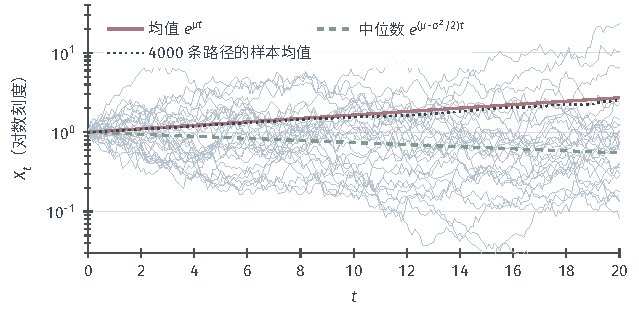
\includegraphics[width=105mm]{figures/03-optimization-evolution-and-signals/02-processes-and-trajectory-evolution/tikz/ctsp-gbm-mean-median/figure.pdf}
  \caption{几何Brownian运动的均值与中位数（纵轴为对数刻度）。$\mu=0.05$，$\sigma=0.4$，$X_0=1$，由显式解在网格上精确生成，固定随机种子。细线是$4000$条路径中的前$30$条；红线为均值$e^{\mu t}$，绿虚线为中位数$e^{(\mu-\sigma^2/2)t}$，点线为$4000$条路径的样本均值。路径主要沿下降的中位数分布，均值由少数大值决定。}
  \label{fig:ctsp-gbm-mean-median}
\end{figure}

\paragraph{Ornstein--Uhlenbeck过程}
第二个基本模型描述带回复力的波动：状态偏离平衡位置时被线性地拉回，同时受到强度恒定的噪声。
\begin{equation}
  \mathrm dX_t=-\lambda X_t\,\mathrm dt+\sigma\,\mathrm dW_t,\qquad\lambda>0 .
  \label{eq:ctsp-ou}
\end{equation}
这是\term{Ornstein--Uhlenbeck过程}（Ornstein--Uhlenbeck process），简称OU过程。求解时像常微分方程一样乘积分因子$e^{\lambda t}$。对$V(t,x)=e^{\lambda t}x\in C^{2,1}$用Itô公式，$\partial_tV=\lambda e^{\lambda t}x$，$\partial_xV=e^{\lambda t}$，$\partial_{xx}V=0$，所以
\[
  \mathrm d\bigl(e^{\lambda t}X_t\bigr)=\lambda e^{\lambda t}X_t\,\mathrm dt+e^{\lambda t}(-\lambda X_t\,\mathrm dt+\sigma\,\mathrm dW_t)=\sigma e^{\lambda t}\,\mathrm dW_t .
\]
二阶修正为零，因为$V$关于$x$是线性的。积分得
\begin{equation}
  X_t=e^{-\lambda t}X_0+\sigma\int_0^te^{-\lambda(t-s)}\,\mathrm dW_s .
  \label{eq:ctsp-ou-solution}
\end{equation}
设$X_0$平方可积且独立于$W$。随机积分的被积函数是确定的，由上一节的结论它是均值零、方差$\sigma^2\int_0^te^{-2\lambda(t-s)}\,\mathrm ds$的高斯变量，于是
\begin{equation}
  \mathbb EX_t=e^{-\lambda t}\mathbb EX_0,\qquad
  \operatorname{Var}(X_t)=e^{-2\lambda t}\operatorname{Var}(X_0)+\frac{\sigma^2}{2\lambda}\bigl(1-e^{-2\lambda t}\bigr).
  \label{eq:ctsp-ou-moments}
\end{equation}
对$s\leq t$，把式~\eqref{eq:ctsp-ou-solution}从$s$开始重写，$X_t=e^{-\lambda(t-s)}X_s+\sigma\int_s^te^{-\lambda(t-r)}\,\mathrm dW_r$，后一项独立于$\mathcal F_s$，所以$\operatorname{Cov}(X_s,X_t)=e^{-\lambda(t-s)}\operatorname{Var}(X_s)$：记忆按速率$\lambda$指数消退。

两个机制在式~\eqref{eq:ctsp-ou-moments}中清楚分开：回复力使初值的均值与方差按$e^{-\lambda t}$、$e^{-2\lambda t}$衰减，持续的噪声不断注入新的方差，二者平衡于$\sigma^2/(2\lambda)$。若初值确定或为与$W$独立的高斯变量，$X_t$本身是高斯的；初值分布取$\mathcal N(0,\sigma^2/(2\lambda))$时，所有时刻的分布都相同。图~\ref{fig:ctsp-ou-envelope}画出从$X_0=3$出发的路径束：均值曲线指数回落，均值加减两倍标准差的包络逐渐并入稳态带。单条路径并不趋于零，它在稳态带内持续波动。

\begin{figure}[htbp]
  \centering
  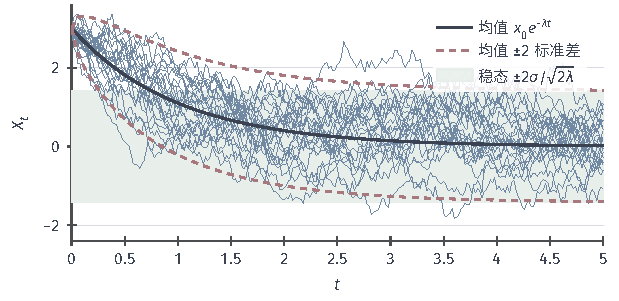
\includegraphics[width=105mm]{figures/03-optimization-evolution-and-signals/02-processes-and-trajectory-evolution/tikz/ctsp-ou-envelope/figure.pdf}
  \caption{OU过程的路径束与矩包络。$\lambda=1$，$\sigma=1$，$X_0=3$；$25$条路径按精确高斯转移在步长$0.01$的网格上生成，固定随机种子。黑线为均值$3e^{-t}$，红虚线为均值$\pm2$倍标准差，绿色带为稳态$\pm2\sigma/\sqrt{2\lambda}$。分布收敛到稳态，路径本身继续波动。}
  \label{fig:ctsp-ou-envelope}
\end{figure}

\paragraph{线性加性噪声系统}
OU过程的推导可以推广到向量情形：
\begin{equation}
  \mathrm d\bm X_t=(\bm A_t\bm X_t+\bm c_t)\,\mathrm dt+\bm G_t\,\mathrm d\bm W_t ,
  \label{eq:ctsp-linear-sde}
\end{equation}
其中$\bm A_t\in\mathbb R^{d\times d}$、$\bm c_t\in\mathbb R^d$、$\bm G_t\in\mathbb R^{d\times m}$都是确定的局部可积函数（$\bm G$局部平方可积），初值$\bm X_0$平方可积且独立于$\bm W$。记$\bm\Phi(t,s)$为齐次方程$\dot{\bm x}=\bm A_t\bm x$的状态转移矩阵（第~\ref{chap:ordinary-differential-equations}章），常系数时$\bm\Phi(t,s)=e^{(t-s)\bm A}$。对$\bm\Phi(0,t)\bm X_t$使用乘积法则~\eqref{eq:ctsp-product-rule}：确定的因子$\bm\Phi(0,t)$有限变差，交叉变差为零，并且$\partial_t\bm\Phi(0,t)=-\bm\Phi(0,t)\bm A_t$，漂移中的$\bm A_t\bm X_t$项正好抵消。积分后乘回$\bm\Phi(t,0)$，
\begin{equation}
  \bm X_t=\bm\Phi(t,0)\bm X_0+\int_0^t\bm\Phi(t,s)\bm c_s\,\mathrm ds+\int_0^t\bm\Phi(t,s)\bm G_s\,\mathrm d\bm W_s .
  \label{eq:ctsp-linear-sde-solution}
\end{equation}
最后一项称为随机卷积。

均值$\bm m_t$与协方差$\bm P_t$可以由路径表达式取矩得到，也可以直接由Itô公式推出。后一种做法对$\widetilde{\bm X}=\bm X-\bm m$的外积用乘积法则：漂移部分给出$\bm A\bm P+\bm P\bm A^\top$，二次协变差给出$\bm G\bm G^\top$，随机积分项在二阶矩有限时期望为零。于是
\begin{equation}
  \dot{\bm m}_t=\bm A_t\bm m_t+\bm c_t,\qquad
  \dot{\bm P}_t=\bm A_t\bm P_t+\bm P_t\bm A_t^\top+\bm G_t\bm G_t^\top .
  \label{eq:ctsp-moment-equations}
\end{equation}
第一项传播已有的不确定性，第二项持续注入新的不确定性。若$\bm A$为常矩阵且所有特征值实部为负，$\bm P_t$趋于Lyapunov方程$\bm A\bm P+\bm P\bm A^\top+\bm G\bm G^\top=\bm0$的唯一解。

关于分布形状需要单独说明。若初值是确定向量，或是与$\bm W$独立的高斯向量，式~\eqref{eq:ctsp-linear-sde-solution}的每个分量都是独立高斯对象的线性组合与$L^2$极限，所以任意有限个时刻的状态联合高斯，矩方程~\eqref{eq:ctsp-moment-equations}就完全决定了分布。初值不是高斯时，$\bm X_t$一般也不是高斯的，均值与协方差只是部分摘要。由状态的带噪观测推断状态，即Kalman滤波，留给第~\ref{chap:state-space-estimation}章。

\begin{example}[受噪声驱动的阻尼振子]
  \label{ex:ctsp-damped-oscillator}
  位置$q$与速度$p$满足$\mathrm dq=p\,\mathrm dt$，$\mathrm dp=(-q-p)\,\mathrm dt+\sigma\,\mathrm dW$：弹簧把位置拉回，摩擦使速度衰减，噪声只直接作用在速度上。此时$\bm A=\begin{pmatrix}0&1\\-1&-1\end{pmatrix}$，$\bm G=(0,\sigma)^\top$。$\bm A$的特征值为$(-1\pm\mathrm i\sqrt3)/2$，实部为负。设稳态协方差$\bm P=\begin{pmatrix}p_{1,1}&p_{1,2}\\p_{1,2}&p_{2,2}\end{pmatrix}$，Lyapunov方程的三个分量给出$2p_{1,2}=0$、$p_{2,2}-p_{1,1}-p_{1,2}=0$、$-2(p_{1,2}+p_{2,2})+\sigma^2=0$，解得$\bm P=\frac{\sigma^2}2\bm I$。噪声只进入速度，位置却得到同样大小的方差，并且稳态下位置与速度不相关。
\end{example}

\subsection{跳跃驱动的状态方程}
\label{sec:ctsp-jump-sde}

\paragraph{事件之间连续演化，事件处更新}
加入速率$\lambda$的Poisson驱动$N$，并规定$\bm W$、$N$与初值相互独立，滤过由三者的历史生成。方程
\begin{equation}
  \mathrm d\bm X_t=\bm b(\bm X_{t-})\,\mathrm dt+\bm\sigma(\bm X_{t-})\,\mathrm d\bm W_t+\bm\gamma(\bm X_{t-})\,\mathrm dN_t
  \label{eq:ctsp-jump-sde}
\end{equation}
的含义仍是积分方程，跳跃项按式~\eqref{eq:ctsp-counting-integral}逐事件累计。解要求是右连续有左极限的适应过程。系数在跳前状态$\bm X_{t-}$处取值，这保证跳跃积分的被积过程可预测；在连续部分，$\bm X_{t-}$与$\bm X_t$只在可数个时刻不同，对$\mathrm dt$与$\mathrm d\bm W$积分没有区别。

这个方程有一个直观的构造。设到达时刻为$T_1<T_2<\cdots$。在$[0,T_1)$上解扩散方程$\mathrm d\bm X=\bm b\,\mathrm dt+\bm\sigma\,\mathrm d\bm W$；在$T_1$处令$\bm X_{T_1}=\bm X_{T_1-}+\bm\gamma(\bm X_{T_1-})$；再从这一新状态出发解扩散方程直到$T_2$，如此继续。若扩散部分满足定理~\ref{thm:ctsp-sde-existence}或定理~\ref{thm:ctsp-nonexplosion}的条件，$\bm\gamma$是有限值的可测函数，有限时段内又只有有限个事件，这一有限次拼接就给出存在且唯一的解。

同一个模型也可以用补偿驱动写出。代入$\mathrm dN=\mathrm d\widetilde N+\lambda\,\mathrm dt$，
\[
  \mathrm d\bm X_t=\bigl[\bm b(\bm X_{t-})+\lambda\bm\gamma(\bm X_{t-})\bigr]\mathrm dt+\bm\sigma(\bm X_{t-})\,\mathrm d\bm W_t+\bm\gamma(\bm X_{t-})\,\mathrm d\widetilde N_t .
\]
补偿形式的漂移多出$\lambda\bm\gamma$，表示跳跃的平均效果；如果只把$\mathrm dN$换成$\mathrm d\widetilde N$而不改漂移，描述的就是另一个模型。

\begin{example}[散粒噪声]
  \label{ex:ctsp-shot-noise}
  考虑$\mathrm dX=-X_{t-}\,\mathrm dt+\sigma\,\mathrm dW_t+c\,\mathrm dN_t$：状态连续泄漏，受到连续的小扰动，并在每个事件时刻增加$c$。均值$m_t=\mathbb EX_t$满足$\dot m=-m+\lambda c$，长期趋于$\lambda c$。对$X^2$使用跳跃Itô公式~\eqref{eq:ctsp-jump-ito}，每次事件使平方增加$(x+c)^2-x^2=2cx+c^2$，所以
  \[
    \frac{\mathrm d}{\mathrm dt}\mathbb EX_t^2=-2\,\mathbb EX_t^2+\sigma^2+\lambda(2cm_t+c^2).
  \]
  稳态下$\mathbb EX^2=\frac12(\sigma^2+2\lambda^2c^2+\lambda c^2)$，减去$m^2=\lambda^2c^2$，得到稳态方差$\frac12(\sigma^2+\lambda c^2)$。连续噪声贡献$\sigma^2$，跳跃贡献$\lambda c^2$，即单位时间内跳幅平方的平均累计量，与第~\ref{sec:ctsp-compensation}节的可预测二阶累计一致。
\end{example}

\paragraph{仍需检查的条件与主线之外的对象}
存在性与不爆炸仍需逐项检查。连续系数要满足上述增长或Lyapunov条件；跳幅$\bm\gamma$若增长很快，单次跳跃可以把状态送到很远的地方，矩估计需要对跳幅加线性增长条件；若事件强度依赖状态并且可以无界增长，有限时间内就可能发生无穷多次事件，上面的有限拼接论证不再适用。状态依赖的有界强度$\lambda(\bm x)\leq\bar\lambda$可以用稀释法构造，第~\ref{sec:ctsp-jump-simulation}节在模拟时说明。

有限时段内无穷多次小跳跃的Lévy驱动、以及状态本身是空间场的随机偏微分方程，都超出本章主线。前者需要用跳跃测度代替逐事件求和，后者需要把第~\ref{chap:partial-differential-equations}章的弱解理论与随机积分结合；它们沿用本章的可预测性与补偿思想，但存在性与正则性需要另外的工具。

\section{状态分布与首次到达问题}
\label{sec:ctsp-distributions}

上一节逐路径地求解方程：给定一条噪声路径，得到一条状态路径。很多问题并不关心某一条路径，而关心整体规律：某个时刻状态落在哪里的概率，从某处出发最终获得的平均收益，先碰到哪一侧边界的概率，平均要等多久。本节说明，这些量都满足确定性的方程。桥梁是Itô公式中的漂移部分，即生成元；它把随机路径上的平均变成偏微分方程或常微分方程，使第~\ref{chap:partial-differential-equations}章的方法获得概率解释，也让概率方法反过来给出这些方程的解。

\subsection{生成元与测试函数期望}
\label{sec:ctsp-generator-dynkin}

\paragraph{从Itô公式读出生成元}
考虑自治的Itô扩散$\mathrm d\bm X_t=\bm b(\bm X_t)\,\mathrm dt+\bm\sigma(\bm X_t)\,\mathrm d\bm W_t$，记扩散矩阵$\bm a=\bm\sigma\bm\sigma^\top$。对$f\in C^2_c(\mathbb R^d)$（二阶连续可微且支撑有界），Itô公式给出
\[
  f(\bm X_t)=f(\bm X_0)+\int_0^t\mathcal Lf(\bm X_s)\,\mathrm ds+\int_0^t\nabla f(\bm X_s)^\top\bm\sigma(\bm X_s)\,\mathrm d\bm W_s ,
\]
其中$\mathcal L$是式~\eqref{eq:ctsp-diffusion-generator}中的二阶微分算子
\begin{equation}
  \mathcal Lf=\sum_ib_i\partial_if+\frac12\sum_{i,j}a_{i,j}\partial_i\partial_jf .
  \label{eq:ctsp-generator-explicit}
\end{equation}
若系数连续，$f$的支撑有界保证随机积分的被积过程有界，它是真鞅；取期望、除以$t$并令$t\downarrow0$，得到$\lim_{t\downarrow0}t^{-1}(\mathbb E_{\bm x}f(\bm X_t)-f(\bm x))=\mathcal Lf(\bm x)$。所以$\mathcal L$正是第~\ref{sec:ctsp-semigroup}节意义下生成元在$C^2_c$上的作用：漂移贡献一阶项，扩散贡献二阶项。

不同驱动在生成元中留下不同形式的项。方程中含有跳跃$\bm\gamma(\bm X_{t-})\,\mathrm dN_t$时，跳跃Itô公式~\eqref{eq:ctsp-jump-ito}在漂移中多出$\lambda[f(\bm x+\bm\gamma(\bm x))-f(\bm x)]$，生成元多了一个有限差项。纯跳跃的连续时间Markov链只有这种项，$\mathcal Lf(i)=\sum_jq_{i,j}[f(j)-f(i)]$，即生成矩阵作用于向量$f$。三种情形放在一起：漂移推动，扩散抹平，跳跃搬运。

\paragraph{Dynkin公式}
在随机时刻停止后，Itô公式的期望形式仍然成立，但需要条件来保证随机积分在停止后的期望为零。

\begin{theorem}[Dynkin公式]
  \label{thm:ctsp-dynkin}
  设$\bm b,\bm\sigma$连续，方程从$\bm x$出发有不爆炸的解。设$f\in C^2(\mathbb R^d)$，$\tau$是停时且$\mathbb E_{\bm x}\tau<\infty$，并且存在有界集合$D$，使停止前$\bm X_t\in D$（或$f$支撑有界）。则
  \begin{equation}
    \mathbb E_{\bm x}f(\bm X_\tau)=f(\bm x)+\mathbb E_{\bm x}\int_0^\tau\mathcal Lf(\bm X_s)\,\mathrm ds .
    \label{eq:ctsp-dynkin}
  \end{equation}
  对$V\in C^{2,1}$，同样的条件下有$\mathbb E_{\bm x}V(\tau,\bm X_\tau)=V(0,\bm x)+\mathbb E_{\bm x}\int_0^\tau(\partial_s+\mathcal L)V(s,\bm X_s)\,\mathrm ds$。
\end{theorem}

\begin{proof}
在$D$的闭包上，$\nabla f^\top\bm\sigma$与$\mathcal Lf$连续因而有界。停止在$\tau\wedge n$，随机积分的被积过程有界，期望为零，于是$\mathbb E_{\bm x}f(\bm X_{\tau\wedge n})=f(\bm x)+\mathbb E_{\bm x}\int_0^{\tau\wedge n}\mathcal Lf(\bm X_s)\,\mathrm ds$。令$n\to\infty$：左端由路径连续与$f$在$\bar D$上有界，用控制收敛；右端被积函数被$\sup_{\bar D}|\mathcal Lf|\cdot\tau$控制，而$\mathbb E\tau<\infty$。含时间的版本只需把Itô公式换成定理~\ref{thm:ctsp-ito-formula}的含时间形式。
\end{proof}

式~\eqref{eq:ctsp-dynkin}称为\term{Dynkin公式}（Dynkin formula）。条件各有用途：$\mathbb E\tau<\infty$保证时间积分可积，状态限制在有界集合中保证函数及其导数有界，从而局部鞅确实是零均值的鞅。去掉其中任一条，等式可能失败；第~\ref{sec:ctsp-optional-sampling}节的首次到达时刻$\tau_a$就是$f(x)=x$、$\mathcal Lf=0$而等式失败的例子，那里$\mathbb E\tau_a=\infty$，路径也不受界。

\paragraph{弱形式的分布演化}
取$\tau=t$为固定时刻，Dynkin公式变成关于状态分布的等式。记$\mu_t$为$\bm X_t$的分布，对$f\in C^2_c$，
\begin{equation}
  \int f\,\mathrm d\mu_t-\int f\,\mathrm d\mu_0=\int_0^t\int\mathcal Lf\,\mathrm d\mu_s\,\mathrm ds .
  \label{eq:ctsp-weak-evolution}
\end{equation}
这个等式不要求$\mu_t$有密度：初值是点质量、扩散退化、或者状态空间是离散的，它都成立。它的含义是，每一个光滑的“读数”$f$，其平均值的变化率等于$\mathcal Lf$的平均值。

反过来问：若一族分布对所有$f\in C^2_c$满足式~\eqref{eq:ctsp-weak-evolution}，或更强地，若过程使$f(\bm X_t)-\int_0^t\mathcal Lf(\bm X_s)\,\mathrm ds$对所有$f\in C^2_c$都是鞅，能否推出过程的规律就是这个方程的解？这称为\term{鞅问题}（martingale problem）。当鞅问题适定，即这样的规律存在且唯一时，答案是肯定的；例如系数有界连续且$\bm a$一致正定时鞅问题适定\scite{math-kallenberg2021probability}。这说明第~\ref{sec:ctsp-semigroup}节的抽象生成元与本节的微分算子之间还隔着一层验证：随机方程给出一个具体的候选生成元，过程的规律是否被它唯一确定，取决于定义域与适定性。

\subsection{后向方程与密度演化}
\label{sec:ctsp-backward-forward}

\paragraph{后向方程：固定终点的平均收益}
设在终点$T$获得收益$g(\bm X_T)$，问从时刻$t$、状态$\bm x$出发的平均收益
\begin{equation}
  u(t,\bm x)=\mathbb E\bigl[g(\bm X_T)\bigm|\bm X_t=\bm x\bigr]
  \label{eq:ctsp-backward-value}
\end{equation}
满足什么方程。这个量对每个起点都要算，用偏微分方程描述它最自然。

关键观察是：沿着路径，$u(t,\bm X_t)=\mathbb E[g(\bm X_T)\mid\mathcal F_t]$（由Markov性质），所以它是一个鞅。若$u\in C^{2,1}$，含时间的Itô公式给出
\[
  \mathrm du(t,\bm X_t)=(\partial_t u+\mathcal Lu)(t,\bm X_t)\,\mathrm dt+\nabla u^\top\bm\sigma\,\mathrm d\bm W_t .
\]
一个连续鞅如果同时是有限变差过程与局部鞅之和，有限变差部分必须为零，于是漂移$(\partial_tu+\mathcal Lu)(t,\bm X_t)$沿路径恒为零。在扩散非退化、状态能到达各处时，这推出
\begin{equation}
  \partial_tu+\mathcal Lu=0,\qquad u(T,\bm x)=g(\bm x),
  \label{eq:ctsp-backward-equation}
\end{equation}
称为后向方程：它从终点条件出发，沿时间向回求解。

上面的推导假设$u$足够光滑，这需要单独论证。实际中更常用的是反方向的验证：若已经找到$u\in C^{2,1}$满足式~\eqref{eq:ctsp-backward-equation}，并且$\nabla u^\top\bm\sigma$满足使随机积分为真鞅的可积条件，那么由Itô公式，$u(s,\bm X_s)$在$[t,T]$上是鞅，比较两端取值即得$u(t,\bm x)=\mathbb E[g(\bm X_T)\mid\bm X_t=\bm x]$。这一论证完全依赖含时间的Itô公式：要验证的是$V(t,\bm X_t)$的漂移为零，而$V$同时依赖时间和状态。

\begin{example}[Brownian运动与热方程]
  \label{ex:ctsp-heat-equation}
  对Brownian运动，$\mathcal L=\frac12\partial_{xx}$，后向方程是$\partial_tu+\frac12\partial_{xx}u=0$，即时间反向的热方程。取$g(x)=x^2$，$u(t,x)=\mathbb E[(x+W_T-W_t)^2]=x^2+(T-t)$，直接核对$\partial_tu+\frac12\partial_{xx}u=-1+1=0$。一般地，$u(t,x)=\int g(y)p_{T-t}(x,y)\,\mathrm dy$，其中$p$是式~\eqref{eq:ctsp-heat-kernel}的热核；这正是第~\ref{chap:partial-differential-equations}章用热核表示的热方程解，只是这里把热核读作转移密度，把解读作平均收益。
\end{example}

\paragraph{前向方程：分布的流动}
后向方程关心“从哪里出发”，以出发状态为变量；前向方程关心“流到哪里”，以到达状态为变量。若$\mu_t$对Lebesgue测度有密度$p(t,\bm x)$，把弱形式~\eqref{eq:ctsp-weak-evolution}中的导数通过分部积分从$f$移到$p$上：漂移项分部积分一次，扩散项两次。测试函数支撑有界，边界项消失，得到
\[
  \int f\,\partial_tp\,\mathrm d\bm x=\int f\Bigl[-\sum_i\partial_i(b_ip)+\frac12\sum_{i,j}\partial_i\partial_j(a_{i,j}p)\Bigr]\mathrm d\bm x .
\]
对所有$f\in C^2_c$成立，所以在分布意义下
\begin{equation}
  \partial_tp=-\sum_i\partial_i(b_ip)+\frac12\sum_{i,j}\partial_i\partial_j(a_{i,j}p),
  \label{eq:ctsp-fokker-planck}
\end{equation}
这就是\term{Fokker--Planck方程}，也称前向Kolmogorov方程。右端的算子是$\mathcal L$的形式伴随$\mathcal L^*$。

把右端写成散度形式$\partial_tp=-\nabla\cdot\bm J$，其中概率流$J_i=b_ip-\frac12\sum_j\partial_j(a_{i,j}p)$，方程就是一条守恒律：某处密度的增减等于概率流的净流入。对全空间积分并假设概率流在无穷远处足够快地消失，得到$\frac{\mathrm d}{\mathrm dt}\int p\,\mathrm d\bm x=0$，总质量守恒。有界区域上的模型还需要边界条件：反射边界要求法向概率流为零，吸收边界要求边界上密度为零，后者使区域内的总质量随时间减少。

\begin{example}[OU密度的流动]
  \label{ex:ctsp-ou-density}
  对$\mathrm dX=-\lambda X\,\mathrm dt+\sigma\,\mathrm dW$，Fokker--Planck方程为$\partial_tp=\partial_x(\lambda xp)+\frac{\sigma^2}2\partial_{xx}p$。从$x_0$出发，由第~\ref{sec:ctsp-linear-sde}节的显式解，$p(t,\cdot)$是$\mathcal N(x_0e^{-\lambda t},\sigma^2(1-e^{-2\lambda t})/(2\lambda))$的密度，可以逐项代入核对。令$\partial_tp=0$并要求概率流为零，$\lambda xp+\frac{\sigma^2}2p'=0$，解得稳态密度$p\propto\exp\{-\lambda x^2/\sigma^2\}$，即$\mathcal N(0,\sigma^2/(2\lambda))$。图~\ref{fig:ctsp-fokker-planck-snapshots}画出$\lambda=1,\sigma=1,x_0=3$时的几个时间截面：起初是集中在$3$附近的窄峰，随后峰顶向左漂移、宽度增加，最后停在稳态上。
\end{example}

\begin{figure}[htbp]
  \centering
  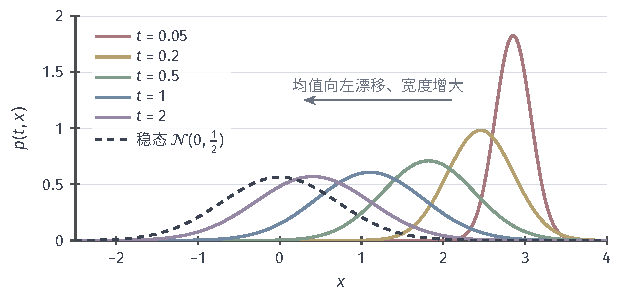
\includegraphics[width=105mm]{figures/03-optimization-evolution-and-signals/02-processes-and-trajectory-evolution/tikz/ctsp-fokker-planck-snapshots/figure.pdf}
  \caption{Fokker--Planck方程的时间截面（解析解，无模拟）。模型为$\mathrm dX=-X\,\mathrm dt+\mathrm dW$，从$x_0=3$出发，$p(t,\cdot)=\mathcal N(3e^{-t},(1-e^{-2t})/2)$。各色曲线为$t=0.05,0.2,0.5,1,2$的密度，黑虚线为稳态$\mathcal N(0,\frac12)$。漂移把概率质量向原点搬运，扩散把它摊开，二者在稳态处平衡。}
  \label{fig:ctsp-fokker-planck-snapshots}
\end{figure}

\paragraph{两个方程的对偶与适用条件}
后向方程与前向方程是同一个演化的两种描述。设$u$解后向方程，$p$解前向方程，则$\frac{\mathrm d}{\mathrm dt}\int u(t,\bm x)p(t,\bm x)\,\mathrm d\bm x=\int(\partial_tu\,p+u\,\partial_tp)\,\mathrm d\bm x=\int(-\mathcal Lu\cdot p+u\cdot\mathcal L^*p)\,\mathrm d\bm x=0$。也就是说$\mathbb Eu(t,\bm X_t)$与$t$无关，在$t=T$处等于$\mathbb Eg(\bm X_T)$。

从弱形式到式~\eqref{eq:ctsp-fokker-planck}的逐点形式，需要密度存在并且足够光滑，系数也要可微。系数光滑有界、并且扩散\term{一致椭圆}（uniformly elliptic），即$\bm a\succeq c\bm I$对某个常数$c>0$成立，是保证正时刻光滑密度的一组常用充分条件。扩散退化时，概率可以停留在低维集合上，例如第~\ref{sec:ctsp-linear-sde}节的阻尼振子只有速度方向直接受噪声，此时密度是否存在要靠漂移把噪声传到其他方向；无法保证时，应停留在弱形式~\eqref{eq:ctsp-weak-evolution}上。有跳跃时，前向方程中还要加入积分项$\lambda\bigl[\text{跳入}\bm x\text{的质量}-p(t,\bm x)\bigr]$，形式取决于跳幅映射。

\subsection{首次到达与随机表示}
\label{sec:ctsp-first-passage}

\paragraph{退出概率与平均退出时间}
设$D\subseteq\mathbb R^d$是有界开区域，$\tau=\inf\{t:\bm X_t\notin D\}$是首次退出时刻。两个典型问题是：从$\bm x$出发，退出时落在边界某一部分$\Gamma$上的概率$u(\bm x)=\mathbb P_{\bm x}(\bm X_\tau\in\Gamma)$，以及平均退出时间$v(\bm x)=\mathbb E_{\bm x}\tau$。

Dynkin公式把它们化为边值问题。设$u\in C^2(D)\cap C(\bar D)$满足
\begin{equation}
  \mathcal Lu=0\ \text{于}D,\qquad u=g\ \text{于}\partial D ,
  \label{eq:ctsp-exit-bvp}
\end{equation}
其中$g$为边界上的给定函数（求退出概率时取$g=\mathbb I_\Gamma$），并且$\mathbb E_{\bm x}\tau<\infty$。对$u$在稍小的区域上使用Dynkin公式，再让区域扩大到$D$，得到$u(\bm x)=\mathbb E_{\bm x}g(\bm X_\tau)$。同样，若$v$满足$\mathcal Lv=-1$于$D$、$v=0$于$\partial D$，则$\mathbb E_{\bm x}\tau=v(\bm x)$：Dynkin公式中的时间积分恰好累计出$\tau$本身。

推导中每个条件都承担具体作用。$\mathbb E_{\bm x}\tau<\infty$保证过程确实会离开并使时间积分可积；当扩散一致椭圆、$D$有界时它成立。$u$在$\bar D$上连续保证边界值确实被取到，这需要边界正则：在非正则的边界点，路径可能贴近边界而不立即离开。$u\in C^2(D)$保证可以使用Itô公式。

\begin{example}[区间上的Brownian运动]
  \label{ex:ctsp-bm-exit-ode}
  $D=(0,1)$，$\mathcal L=\frac12\frac{\mathrm d^2}{\mathrm dx^2}$。退出于$1$的概率满足$\frac12u''=0$、$u(0)=0$、$u(1)=1$，所以$u(x)=x$；平均退出时间满足$\frac12v''=-1$、$v(0)=v(1)=0$，所以$v(x)=x(1-x)$。这与第~\ref{sec:ctsp-optional-sampling}节用鞅算出的式~\eqref{eq:ctsp-exit-probability}、\eqref{eq:ctsp-exit-time}一致：那里构造的两个鞅$X_t$与$X_t^2-t$，正是$\mathcal Lu=0$与$\mathcal Lv=-1$的解沿路径的形式。图~\ref{fig:ctsp-exit-problem}用模拟核对了两个函数。
\end{example}

\begin{figure}[htbp]
  \centering
  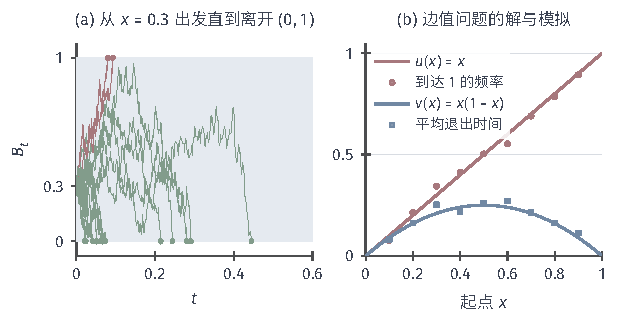
\includegraphics[width=104.5mm]{figures/03-optimization-evolution-and-signals/02-processes-and-trajectory-evolution/tikz/ctsp-exit-problem/figure.pdf}
  \caption{Brownian运动退出区间$(0,1)$。(a)从$x=0.3$出发的$14$条路径，直到离开浅蓝色区域，红色先到达$1$，绿色先到达$0$，圆点为退出位置，为显示只画到$t=0.6$；(b)边值问题的解$u(x)=x$（退出于$1$的概率）与$v(x)=x(1-x)$（平均退出时间），点为每个起点$300$条模拟路径的频率与平均。模拟用步长$2\times10^{-4}$的高斯随机游走并在网格上检测退出，固定随机种子；离散检测会略微推迟退出，平均退出时间因此略有偏高。}
  \label{fig:ctsp-exit-problem}
\end{figure}

加入漂移后，退出概率不再是线性函数。设$\mathrm dX=\mu\,\mathrm dt+\mathrm dW$，$\mu\neq0$，在$(0,1)$中求$u$：方程$\frac12u''+\mu u'=0$的通解为$u=c_1+c_2e^{-2\mu x}$，由边界条件
\[
  \mathbb P_x(\text{先到达}1)=\frac{1-e^{-2\mu x}}{1-e^{-2\mu}} .
\]
$\mu>0$时曲线向上凸起：即使从左端附近出发，向右的漂移也使到达右端的机会显著增加。$\mu\to0$时它回到线性函数$x$。

\paragraph{Feynman--Kac表示}
后向方程可以推广到带“折损”和“流量”的情形。设想沿路径累计收益：在状态$\bm x$处每单位时间获得$f(\bm x)$，同时收益按速率$V(\bm x)\geq0$贴现或衰减，终点再获得$g(\bm X_T)$。

\begin{theorem}[Feynman--Kac表示]
  \label{thm:ctsp-feynman-kac}
  设$\bm b,\bm\sigma$满足定理~\ref{thm:ctsp-sde-existence}的条件，$V\geq0$、$f$、$g$连续有界。若$u\in C^{2,1}([0,T)\times\mathbb R^d)\cap C([0,T]\times\mathbb R^d)$有界，满足
  \begin{equation}
    \partial_tu+\mathcal Lu-Vu+f=0,\qquad u(T,\cdot)=g ,
    \label{eq:ctsp-feynman-kac-pde}
  \end{equation}
  并且$\nabla u^\top\bm\sigma$在每个$[0,T']\times\mathbb R^d$（$T'<T$）上有界，则
  \begin{equation}
    u(t,\bm x)=\mathbb E_{t,\bm x}\Bigl[\int_t^Te^{-\int_t^sV(\bm X_r)\,\mathrm dr}f(\bm X_s)\,\mathrm ds+e^{-\int_t^TV(\bm X_r)\,\mathrm dr}g(\bm X_T)\Bigr].
    \label{eq:ctsp-feynman-kac}
  \end{equation}
\end{theorem}

\begin{proof}
令$E_s=\exp\{-\int_t^sV(\bm X_r)\,\mathrm dr\}$，它是有限变差过程，$\mathrm dE_s=-V(\bm X_s)E_s\,\mathrm ds$，与$u(s,\bm X_s)$的二次协变差为零。由乘积法则与含时间的Itô公式，
\[
  \begin{aligned}
    \mathrm d\bigl[E_su(s,\bm X_s)\bigr]&=E_s\bigl(\partial_su+\mathcal Lu-Vu\bigr)\,\mathrm ds+E_s\nabla u^\top\bm\sigma\,\mathrm d\bm W_s\\
    &=-E_sf(\bm X_s)\,\mathrm ds+E_s\nabla u^\top\bm\sigma\,\mathrm d\bm W_s .
  \end{aligned}
\]
在$[t,T']$上积分，随机积分的被积过程有界，期望为零，于是$u(t,\bm x)=\mathbb E[E_{T'}u(T',\bm X_{T'})+\int_t^{T'}E_sf(\bm X_s)\,\mathrm ds]$。令$T'\uparrow T$，$u$有界连续，$E_s\in(0,1]$，由控制收敛定理得到式~\eqref{eq:ctsp-feynman-kac}。
\end{proof}

式~\eqref{eq:ctsp-feynman-kac}称为\term{Feynman--Kac表示}（Feynman--Kac representation），它有一个直观的读法：$V$是“死亡率”，路径在每段短时间$\mathrm dr$内以概率$V\,\mathrm dr$被杀死，$E_s$就是活到$s$的概率；$f$是存活期间的收益率，$g$是存活到终点的奖励。$V$取常数$r$、$f=0$时，式~\eqref{eq:ctsp-feynman-kac}化为贴现收益$u=e^{-r(T-t)}\mathbb E_{t,\bm x}g(\bm X_T)$。这个表示把偏微分方程的解写成随机路径上的平均，因而可以用模拟路径计算，也可以反过来用PDE的数值方法计算路径期望。

表示的适用范围需要说清。方程中的二阶部分必须是某个扩散的生成元，即扩散矩阵半正定；方程必须是线性的；定理把经典解的存在当作假设，存在性本身要由PDE理论另行保证。超出这些条件的方程，例如非线性方程或对$u$的梯度有非线性依赖的方程，不能直接用Brownian路径的期望表示。

\section{稳定性与长期行为}
\label{sec:ctsp-stability}

长时间运行之后会发生什么？这个问题对随机系统有两种不同的问法。第一种沿用第~\ref{chap:ordinary-differential-equations}章的视角：把同一噪声下的两条解放在一起，问初值扰动是否衰减，平衡点是否吸引附近的路径。第二种是第~\ref{chap:discrete-time-stochastic-processes}章的视角：不看单条路径，问状态的分布是否趋于一个不变分布，时间平均是否趋于总体平均。OU过程的路径不收敛到任何点，分布却收敛；乘性噪声的线性方程几乎每条路径都趋于零，二阶矩却可能发散。本节把这些情形分开讨论。

\subsection{随机状态的稳定性}
\label{sec:ctsp-stochastic-stability}

\paragraph{同一噪声下的两条解}
比较初值扰动的影响，最直接的办法是用同一条Brownian路径驱动两个初值。对加性噪声的线性方程$\mathrm dX=-\lambda X\,\mathrm dt+\sigma\,\mathrm dW$，两条解之差满足$\mathrm d(X^x-X^y)=-\lambda(X^x-X^y)\,\mathrm dt$，噪声完全抵消，$X^x_t-X^y_t=e^{-\lambda t}(x-y)$。初值的影响按确定性的速率消失，而每条路径仍在不断波动。

若噪声依赖状态，差也会带上噪声。设$\bm b(\bm0)=\bm0$、$\bm\sigma(\bm0)=\bm0$，于是$\bm0$是一个平衡解：从零出发的路径永远停在零。问题是附近的路径是否被吸引到零。随机情形有几种不等价的稳定要求，需要分别命名。
\begin{itemize}
  \item \term{依概率稳定}（stability in probability）：对任意$\varepsilon,\eta>0$，存在$\delta>0$，使$\|\bm x\|_2<\delta$时$\mathbb P_{\bm x}(\sup_{t\geq0}\|\bm X_t\|_2>\varepsilon)<\eta$。
  \item \term{几乎必然指数稳定}（almost sure exponential stability）：存在$\kappa>0$，使对所有初值，$\limsup_{t\to\infty}t^{-1}\log\|\bm X_t\|_2\leq-\kappa$几乎必然。
  \item $p$阶\term{矩指数稳定}（moment exponential stability），其中$p>0$：存在$C,\kappa>0$，使$\mathbb E_{\bm x}\|\bm X_t\|_2^p\leq C\|\bm x\|_2^pe^{-\kappa t}$；$p=2$时称均方指数稳定。
\end{itemize}

\paragraph{标量乘性噪声}
最简单的例子已经把这几种稳定区分开了。考虑$\mathrm dX=bX\,\mathrm dt+\sigma X\,\mathrm dW$，$X_0=x\neq0$。由第~\ref{sec:ctsp-linear-sde}节的几何Brownian运动公式，$X_t=x\exp\{(b-\sigma^2/2)t+\sigma W_t\}$，于是
\begin{equation}
  \frac1t\log|X_t|=\frac{\log|x|}t+b-\frac{\sigma^2}2+\sigma\frac{W_t}t\longrightarrow b-\frac{\sigma^2}2\quad\text{几乎必然},
  \label{eq:ctsp-lyapunov-exponent}
\end{equation}
\begin{equation}
  \mathbb E|X_t|^p=|x|^p\exp\Bigl\{p\Bigl(b+\frac{(p-1)\sigma^2}2\Bigr)t\Bigr\}.
  \label{eq:ctsp-pth-moment}
\end{equation}
第二式由$\mathbb Ee^{p\sigma W_t}=e^{p^2\sigma^2t/2}$得到。几乎必然指数稳定当且仅当$b<\sigma^2/2$，均方指数稳定当且仅当$2b+\sigma^2<0$。

取$b=-1$、$\sigma^2=3$。无噪声时$\dot x=-x$稳定；加噪声后，几乎必然指数为$-2.5$，路径比无噪声时衰减得更快，但二阶矩指数为$2b+\sigma^2=1>0$，$\mathbb EX_t^2$指数增长。图~\ref{fig:ctsp-multiplicative-stability}画出了这一对照：每条路径的$\log|X_t|$都沿斜率$-2.5$下降，均方却在上升。原因是$\log X_t$服从正态分布，$X_t^2$是对数正态的，它的期望由极少数极大值支配；这些路径出现的概率随时间迅速变小，但它们对二阶矩的贡献增长得更快。反过来，$b=0.5$、$\sigma=1.5$时，确定性部分不稳定，几乎必然指数却是$0.5-1.125<0$：噪声使路径几乎必然衰减。所以“确定性部分稳定”既不是随机稳定的充分条件，也不是必要条件，而且不同稳定概念需要分别检查。

\begin{figure}[htbp]
  \centering
  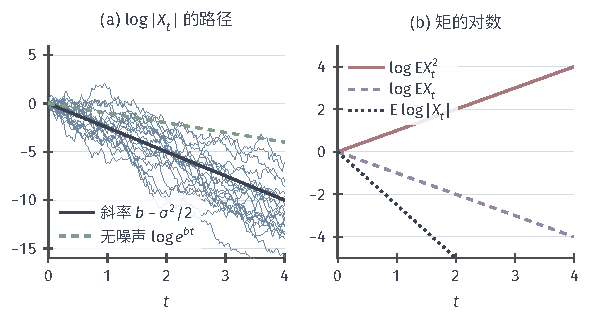
\includegraphics[width=100mm]{figures/03-optimization-evolution-and-signals/02-processes-and-trajectory-evolution/tikz/ctsp-multiplicative-stability/figure.pdf}
  \caption{乘性噪声下几乎必然稳定与均方不稳定并存。模型$\mathrm dX=bX\,\mathrm dt+\sigma X\,\mathrm dW$，$b=-1$，$\sigma^2=3$，$X_0=1$。(a)$20$条路径的$\log|X_t|$（由显式解在网格上生成，固定随机种子），黑线为斜率$b-\sigma^2/2=-2.5$，绿虚线为无噪声解；(b)解析的矩指数：$\log\mathbb EX_t^2=(2b+\sigma^2)t$上升，$\log\mathbb EX_t=bt$与$\mathbb E\log|X_t|=(b-\sigma^2/2)t$下降。}
  \label{fig:ctsp-multiplicative-stability}
\end{figure}

式~\eqref{eq:ctsp-pth-moment}还揭示了两类稳定之间的联系。矩指数$p(b+(p-1)\sigma^2/2)$在$p=0$处为零，对$p$的导数为$b-\sigma^2/2$，恰为几乎必然指数。所以几乎必然指数稳定当且仅当对充分小的$p>0$有$p$阶矩指数稳定；阶数越高，越容易被罕见的大值破坏。

\paragraph{随机Lyapunov函数}
没有显式解时，第~\ref{chap:ordinary-differential-equations}章的Lyapunov方法仍然可用，只是沿路径的导数要换成Itô公式的漂移，即生成元$\mathcal LV$。

\begin{theorem}[矩稳定的Lyapunov判据]
  \label{thm:ctsp-lyapunov-moment}
  设系数局部Lipschitz，$\bm b(\bm0)=\bm0$，$\bm\sigma(\bm0)=\bm0$。若存在$V\in C^2(\mathbb R^d)$与常数$c_1,c_2,c_3>0$、$p>0$，使
  \[
    c_1\|\bm x\|_2^p\leq V(\bm x)\leq c_2\|\bm x\|_2^p,\qquad\mathcal LV(\bm x)\leq-c_3V(\bm x)
  \]
  对所有$\bm x$成立，则解不爆炸，并且$\mathbb E_{\bm x}\|\bm X_t\|_2^p\leq(c_2/c_1)\|\bm x\|_2^pe^{-c_3t}$，即零解$p$阶矩指数稳定。
\end{theorem}

\begin{proof}
不爆炸由定理~\ref{thm:ctsp-nonexplosion}（取常数$c=0$）得到。对$U(t,\bm x)=e^{c_3t}V(\bm x)$使用含时间的Itô公式，漂移为$e^{c_3t}(c_3V+\mathcal LV)\leq0$。在$\tau_R\wedge t$停止，随机积分期望为零，$\mathbb E[e^{c_3(\tau_R\wedge t)}V(\bm X_{\tau_R\wedge t})]\leq V(\bm x)$；令$R\to\infty$，Fatou引理给出$\mathbb E[e^{c_3t}V(\bm X_t)]\leq V(\bm x)$，再代入$V$的上下界。
\end{proof}

以标量乘性模型核对：$V(x)=x^2$时$\mathcal LV=(2b+\sigma^2)x^2$，判据给出均方稳定当且仅当$2b+\sigma^2<0$，与显式计算一致。判据的证明串起了本章前面的几步：局部Lipschitz给出到爆炸为止的解，Lyapunov函数排除爆炸，含时间的Itô公式与停止保证期望可以取，Fatou引理去掉截断。几乎必然稳定可以用同样的思路处理$\log V$，但所需条件不同，须另行检查；不同的结论对应不同的函数控制与噪声条件，不能笼统地称为“稳定”。

\subsection{不变分布与分布趋稳}
\label{sec:ctsp-invariant}

\paragraph{半群的不动点}
离散章区分了三件事：不变分布存在，不变分布唯一，从给定初值出发的分布收敛到它。连续时间的不变性写成对所有时长同时成立的不动点条件：若
\[
  \mu P_t=\mu\qquad\text{对所有 }t\geq0 ,
\]
就称$\mu$为\term{不变分布}（invariant distribution）。以$\mu$为初始分布的过程在每个时刻都有同样的边缘分布，并且由时间齐次性，整个过程关于时间平移的联合规律不变。

验证不变性时，通常不直接计算$\mu P_t$，而检查生成元。由弱形式~\eqref{eq:ctsp-weak-evolution}，若$\mu$不变，则$\int\mathcal Lf\,\mathrm d\mu=0$对所有$f\in C^2_c$成立；有密度时等价于Fokker--Planck方程的稳态$\mathcal L^*p=0$。反方向需要更多条件：$\int\mathcal Lf\,\mathrm d\mu=0$只是候选，要推出$\mu P_t=\mu$，还需鞅问题适定，或$C^2_c$在生成元定义域中足够丰富。连续时间Markov链中这一检验就是$\bm\pi\bm Q=\bm0$；可数状态时还要求链不爆炸。

\paragraph{OU过程的稳态}
OU过程可以把候选验证与实际收敛都算出来。第~\ref{sec:ctsp-backward-forward}节由稳态Fokker--Planck方程得到候选$\pi=\mathcal N(0,\sigma^2/(2\lambda))$。实际收敛由显式解给出：$X_t=e^{-\lambda t}X_0+Z_t$，其中$Z_t=\sigma\int_0^te^{-\lambda(t-s)}\,\mathrm dW_s\sim\mathcal N(0,\sigma^2(1-e^{-2\lambda t})/(2\lambda))$与$X_0$独立。第一项几乎必然趋于零，第二项的分布趋于$\pi$，所以对任何初值分布，$X_t$的分布都收敛到$\pi$，$\pi$也因此是唯一的不变分布。

收敛速度可以用同一噪声的耦合读出。两个从不同初值出发、由同一$W$驱动的解满足$|X^x_t-X^y_t|=e^{-\lambda t}|x-y|$。若让$X^y_0$服从$\pi$，它在所有时刻都服从$\pi$，于是$X^x_t$与一个服从$\pi$的变量之间的均方距离不超过$e^{-\lambda t}(\mathbb E|x-X^y_0|^2)^{1/2}$。这个耦合给出分布之间按速率$\lambda$的指数收敛：二阶Wasserstein距离定义为两个分布的所有耦合下均方根距离的下确界，所以它不超过上面这个特定耦合给出的$e^{-\lambda t}(\mathbb E|x-X^y_0|^2)^{1/2}$。这一距离及其性质可参考\BookChapterRef{chap:information-theory-and-statistical-geometry}{卷四“信息论与统计几何”章}。

\paragraph{一般扩散还需检查什么}
形式上解出稳态方程$\mathcal L^*p=0$，离得到“过程收敛到$p$”还有好几步，每一步都可能失败。
\begin{itemize}
  \item 解可能不可归一化。Brownian运动的生成元$\frac12\partial_{xx}$满足$\int\mathcal Lf\,\mathrm dx=0$，Lebesgue测度是不变测度，但它不是概率分布；Brownian运动没有不变分布，$W_t$的分布不断摊开。
  \item 不变分布可能不唯一。设$\mathrm dX=X(1-X)\,\mathrm dW$，$X_0\in[0,1]$：噪声在$0$与$1$处消失，$\delta_0$与$\delta_1$都是不变分布，路径最终被吸收到其中一个端点，吸收到哪一个取决于初值。扩散退化使过程不可约性失败。
  \item 过程本身可能不良定，例如在有限时间爆炸，或在有界区域上缺少与模型一致的边界条件。
\end{itemize}
一组常用的充分条件是：系数光滑，扩散一致椭圆，并且存在随状态增长而趋于无穷的Lyapunov函数$V$，使$\mathcal LV\leq-cV+d$（$c>0$）。前者保证过程能以正概率到达各处，因而至多一个不变分布；后者把过程拉回有界区域，保证不变分布存在并且从任何初值出发的分布收敛到它\scite{math-meyn2009markov}。存在、唯一与收敛应分别论证，不能由形式稳态密度直接推出。

\subsection{连续时间平均与波动}
\label{sec:ctsp-time-average}

\paragraph{时间平均的遍历定理}
离散章的遍历定理说，平稳遍历时$n^{-1}\sum_{k<n}f(X_k)$几乎必然趋于$\int f\,\mathrm d\pi$。连续时间把样本平均换成单位时间的累计
\begin{equation}
  \bar f_T=\frac1T\int_0^Tf(X_t)\,\mathrm dt .
  \label{eq:ctsp-time-average}
\end{equation}
渐进可测性保证积分是随机变量。若$X$以不变分布$\pi$启动且平稳过程是遍历的，对$\pi$可积的$f$有$\bar f_T\to\int f\,\mathrm d\pi$几乎必然；对满足适当回返条件（例如正Harris常返）的Markov过程，结论对任意初值成立\scite{math-meyn2009markov}。OU过程中，$\bar X_T\to0$，$\overline{X^2}_T\to\sigma^2/(2\lambda)$。

一个自然的捷径是只在等间隔时刻$kh$观察，把连续时间问题化为离散链$(X_{kh})_k$，称为\term{骨架链}（skeleton chain）。骨架链的不变分布包含连续过程的不变分布，但遍历性不一定传递。确定性的例子最清楚：单位圆上的匀速旋转$X_t=(\cos t,\sin t)$，均匀分布不变，连续时间平均对任何连续函数都收敛到均匀分布下的平均；取$h=2\pi$，骨架链却停在原地，样本平均只是初值处的函数值。随机过程中扩散非退化通常能排除这种共振，但需要检查，而不是默认骨架链与连续过程等价。

\paragraph{长期方差与Poisson方程}
遍历定理只说平均会收敛，不说误差有多大。设$X$平稳，$f$平方可积，记$C(s)=\operatorname{Cov}_\pi(f(X_0),f(X_s))$。由平稳性与Fubini定理，
\[
  \operatorname{Var}\Bigl(\int_0^Tf(X_t)\,\mathrm dt\Bigr)=\int_0^T\!\!\int_0^TC(|t-s|)\,\mathrm ds\,\mathrm dt=2\int_0^T(T-s)C(s)\,\mathrm ds .
\]
若$\int_0^\infty|C(s)|\,\mathrm ds<\infty$，则$T\operatorname{Var}(\bar f_T)\to\sigma_f^2=2\int_0^\infty C(s)\,\mathrm ds$，极限$\sigma_f^2$称为\term{长期方差}（asymptotic variance）。这与离散章的协方差和相对应：相关越持久，有效的独立观测越少。OU过程取$f(x)=x$，$C(s)=\frac{\sigma^2}{2\lambda}e^{-\lambda s}$，于是$\sigma_f^2=\sigma^2/\lambda^2$。

中心极限定理需要比方差公式更多的结构。一条有用的路线是解Poisson方程：找$g$使
\begin{equation}
  -\mathcal Lg=f-\int f\,\mathrm d\pi .
  \label{eq:ctsp-poisson-equation}
\end{equation}
对$g(X_t)$使用Itô公式，$g(X_T)-g(X_0)=\int_0^T\mathcal Lg(X_t)\,\mathrm dt+M_T$，其中$M_T=\int_0^T\nabla g^\top\bm\sigma\,\mathrm d\bm W$。整理得
\[
  \int_0^T\Bigl(f(X_t)-\int f\,\mathrm d\pi\Bigr)\mathrm dt=g(X_0)-g(X_T)+M_T .
\]
时间平均的误差被拆成有界的边界项与一个鞅。若$g$满足适当的矩条件，边界项除以$\sqrt T$后趋零，鞅的中心极限定理给出$\sqrt T(\bar f_T-\int f\,\mathrm d\pi)\Rightarrow\mathcal N(0,\sigma_f^2)$，其中$\sigma_f^2=\int\|\bm\sigma^\top\nabla g\|_2^2\,\mathrm d\pi$，即鞅的平均二次变差速率。仍以OU过程、$f(x)=x$核对：$g(x)=x/\lambda$满足$-\mathcal Lg=-(-\lambda x)/\lambda=x$，$\sigma_f^2=\sigma^2/\lambda^2$，与协方差积分的结果一致。

这条路线的每一步都依赖条件：Poisson方程可解，解有足够的矩，鞅中心极限定理的条件成立。遍历性本身不保证这些，连续时间的遍历过程也可以没有中心极限定理。第~\ref{sec:ctsp-sampling}节用这里的长期方差为时间平均估计标准误；协方差函数的频谱表示与估计留给第~\ref{chap:signal-analysis}章。

\section{随机路径的数值模拟}
\label{sec:ctsp-numerical}

除了少数线性模型，随机微分方程没有显式解，需要在计算机上生成近似路径。本节研究一个已经给定的连续时间模型怎样离散：扩散部分按时间步进，跳跃部分按事件或网格处理，误差则按两种不同的目标衡量——近似路径是否贴近真实路径，近似分布的期望是否贴近真实期望。这里的模型是给定的，任务是忠实地模拟它；下一节反过来设计一个过程去采样给定的目标分布，两类任务的误差含义不同。

\subsection{扩散方程的时间步进}
\label{sec:ctsp-time-stepping}

\paragraph{Euler--Maruyama方法}
第~\ref{chap:ordinary-differential-equations}章的显式Euler方法在每一步冻结左端点的变化率。随机方程沿用同一想法：在每个小区间上把漂移与扩散系数冻结在左端点。取步长$h$、网格$t_k=kh$，令$\widehat{\bm X}_0=\bm X_0$，
\begin{equation}
  \widehat{\bm X}_{k+1}=\widehat{\bm X}_k+\bm b(t_k,\widehat{\bm X}_k)\,h+\bm\sigma(t_k,\widehat{\bm X}_k)\,\Delta\bm W_k,\qquad\Delta\bm W_k=\sqrt h\,\bm\xi_k ,
  \label{eq:ctsp-euler-maruyama}
\end{equation}
其中$\bm\xi_k\sim\mathcal N(\bm0,\bm I_m)$相互独立，并独立于初值。这称为\term{Euler--Maruyama方法}（Euler--Maruyama method）。冻结在左端点与Itô积分的左端点取样一致，这一点很重要：若把扩散系数取在右端点或中点，离散极限会是另一种积分约定下的方程。

噪声项乘的是$\sqrt h$而不是$h$。每一步的扩散增量方差为$h\,\bm\sigma\bm\sigma^\top$，在长度为$T$的时段上累计$T/h$步，方差的总和保持$T\bm\sigma\bm\sigma^\top$的量级；这正是第~\ref{sec:ctsp-brownian}节的$\sqrt{\Delta t}$缩放。若误写成$h\bm\xi_k$，累计方差按$h$趋零，模拟出来的是无噪声的常微分方程。每一步的计算量是一次漂移与扩散系数求值、$m$个独立高斯数，以及一次$d\times m$的矩阵向量乘法。

以OU过程为例可以看清离散化引入了什么。Euler--Maruyama给出$\widehat X_{k+1}=(1-\lambda h)\widehat X_k+\sigma\sqrt h\,\xi_k$，而精确转移是$X_{t_{k+1}}=e^{-\lambda h}X_{t_k}+\sigma\sqrt{(1-e^{-2\lambda h})/(2\lambda)}\,\xi_k$。两者在$h\to0$时一阶一致，但前者只有在$|1-\lambda h|<1$即$0<h<2/\lambda$时才稳定，其稳态方差为$\sigma^2h/[1-(1-\lambda h)^2]=\sigma^2/[\lambda(2-\lambda h)]$，而不是$\sigma^2/(2\lambda)$。第~\ref{sec:ctsp-error-types}节将回到这一长期偏差。

\paragraph{Itô--Taylor展开与Milstein修正}
Euler--Maruyama的误差主要来自扩散系数在区间内的变化。以标量自治方程为例，在$[t_k,t_{k+1}]$内，对$\sigma(X_s)$用Itô公式展开，主导部分是
\[
  \sigma(X_s)\approx\sigma(X_{t_k})+\sigma'(X_{t_k})\sigma(X_{t_k})(W_s-W_{t_k}),
\]
漂移的变化与时间项都是更高阶的。代入$\int_{t_k}^{t_{k+1}}\sigma(X_s)\,\mathrm dW_s$，多出的一项含迭代积分$\int_{t_k}^{t_{k+1}}(W_s-W_{t_k})\,\mathrm dW_s=\frac12[(\Delta W_k)^2-h]$，这正是式~\eqref{eq:ctsp-int-w-dw}在一个小区间上的版本。于是得到\term{Milstein方法}（Milstein method）
\begin{equation}
  \widehat X_{k+1}=\widehat X_k+b(\widehat X_k)h+\sigma(\widehat X_k)\Delta W_k+\frac12\sigma(\widehat X_k)\sigma'(\widehat X_k)\bigl[(\Delta W_k)^2-h\bigr].
  \label{eq:ctsp-milstein}
\end{equation}
对几何Brownian运动，修正项为$\frac12\sigma^2\widehat X_k[(\Delta W_k)^2-h]$。加性噪声时$\sigma'=0$，Milstein方法与Euler--Maruyama相同。

修正需要额外的代价。它要求扩散系数可微并计算导数；多维情形一般含有不同Brownian分量之间的迭代积分$\int(W^{(i)}_s-W^{(i)}_{t_k})\,\mathrm dW^{(j)}_s$，其反对称部分（Lévy面积）不能由增量$\Delta\bm W_k$本身算出，需要额外模拟。只有在噪声满足交换条件等特殊结构时，这些项才可以化简掉。

\paragraph{非全局Lipschitz系数}
前面的收敛结论依赖全局Lipschitz与线性增长条件。漂移超线性增长时，即使连续方程不爆炸，显式方法也可能出问题。以$\mathrm dX=-X^3\,\mathrm dt+\mathrm dW$为例，连续方程的漂移强烈地把状态拉回原点；但Euler--Maruyama的确定性部分是$x\mapsto x-hx^3$，当$|x|>\sqrt{2/h}$时$|x-hx^3|=|x|(hx^2-1)>|x|$，状态不但没有被拉回，反而被放大并改变符号，此后每一步都以大约立方的速度增长。一次较大的高斯增量就足以把数值路径推进这一区域，概率虽小，增长却极快，于是数值矩可能失去控制。

常用的补救办法有两类。\term{驯化方法}（taming）把漂移增量限制在可控范围内，例如用$h\bm b(\widehat{\bm X}_k)/(1+h\|\bm b(\widehat{\bm X}_k)\|_2)$代替$h\bm b(\widehat{\bm X}_k)$，使单步漂移位移不超过一；隐式方法在漂移中使用$\widehat{\bm X}_{k+1}$，例如$\widehat X_{k+1}=\widehat X_k-h\widehat X_{k+1}^3+\Delta W_k$，每步解一个标量方程，它对任何$h$都把状态拉回。两者都需要单独证明收敛，不能直接沿用全局Lipschitz情形的结论。

\subsection{跳跃过程的模拟}
\label{sec:ctsp-jump-simulation}

\paragraph{事件驱动模拟}
对有限活动的跳跃扩散~\eqref{eq:ctsp-jump-sde}，最忠实的做法是把跳跃时刻放进网格。先依次抽取独立的$\operatorname{Exp}(\lambda)$等待时间得到跳跃时刻$T_1<T_2<\cdots$，并为每次跳跃抽取所需的标记；然后在相邻跳跃之间用某种扩散步进推进连续部分，最后一步的长度截到跳跃时刻；到达$T_j$时用跳前状态更新，$\bm X_{T_j}=\bm X_{T_j-}+\bm\gamma(\bm X_{T_j-})$。跳时与跳幅都被精确保留，误差只来自跳跃之间的扩散步进；若扩散部分可以精确求解（例如OU过程），整个模拟就是精确的。

若事件强度依赖状态，$\lambda(\bm x)\leq\bar\lambda$，可以用\term{稀释法}（thinning）：先以常数速率$\bar\lambda$生成候选事件，在候选时刻以概率$\lambda(\bm X_{t-})/\bar\lambda$接受为真实事件，否则丢弃。由于Poisson过程的独立稀释仍是计数过程，且被接受的候选在短时间内的发生概率为$\bar\lambda h\cdot\lambda(\bm x)/\bar\lambda=\lambda(\bm x)h$，接受的事件恰好具有所需的强度。上界$\bar\lambda$越松，被丢弃的候选越多，计算越浪费。

\paragraph{固定网格的近似}
若为了与其他计算对齐而使用固定网格，每一步抽取$\Delta N_k\sim\operatorname{Poisson}(\lambda h)$，并把跳幅冻结在步首：
\[
  \widehat{\bm X}_{k+1}=\widehat{\bm X}_k+\bm b(\widehat{\bm X}_k)h+\bm\sigma(\widehat{\bm X}_k)\Delta\bm W_k+\bm\gamma(\widehat{\bm X}_k)\Delta N_k .
\]
这引入两类新增误差。一是时刻错位：跳跃被推迟到所在步的末端，错位不超过$h$，在跳跃之间连续部分按错误的状态演化了一段时间。二是步内多次事件：一步内出现两次以上事件的概率约为$(\lambda h)^2/2$，此时冻结的跳幅$\bm\gamma(\widehat{\bm X}_k)$被重复使用，而真实的第二次跳跃应该在第一次跳跃之后的状态处计算。图~\ref{fig:ctsp-jump-event-grid}在同一组噪声与事件下比较了两种做法：跳幅依赖状态时，网格路径在多次事件的格子里明显偏离。

\begin{figure}[htbp]
  \centering
  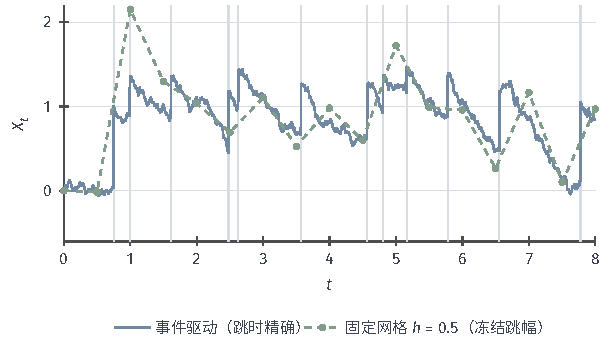
\includegraphics[width=105mm]{figures/03-optimization-evolution-and-signals/02-processes-and-trajectory-evolution/tikz/ctsp-jump-event-grid/figure.pdf}
  \caption{事件驱动与固定网格的跳跃模拟。模型$\mathrm dX=-X\,\mathrm dt+0.25\,\mathrm dW+\gamma(X_-)\,\mathrm dN$，跳幅$\gamma(x)=1-0.6x$依赖跳前状态，事件速率$\lambda=1.2$，固定随机种子。灰色竖线为事件时刻。蓝线在细网格上推进扩散，并在事件时刻精确跳跃；绿色折线用步长$h=0.5$的网格、相同的Brownian增量与每格事件数，跳幅冻结在格首状态。两者的差来自跳时错位与同一格内多次事件。}
  \label{fig:ctsp-jump-event-grid}
\end{figure}

跳跃部分与连续部分的误差来源不同，报告时应分开。精确模拟跳跃而只近似扩散时，误差分析回到上一小节；跳跃也只能近似时（例如强度没有可用的上界，或跳幅分布难以采样），应分别说明跳跃近似与连续步进各自的误差，以及两者怎样随$h$变化。

\subsection{强误差、弱误差与长期偏差}
\label{sec:ctsp-error-types}

\paragraph{两种误差}
衡量数值解的好坏，首先要说清比较的对象。若关心的是单条路径，例如要用模拟路径检验某个依赖路径细节的控制策略，就应当在同一条Brownian路径下比较真解与数值解，即用$\Delta\bm W_k=\bm W_{t_{k+1}}-\bm W_{t_k}$驱动数值格式。终点的\term{强误差}（strong error）定义为$\bigl(\mathbb E\|\bm X_T-\widehat{\bm X}_n\|_2^p\bigr)^{1/p}$，常取$p=1$或$2$。若关心的只是期望，例如某个读数的平均，就不必让两条路径配对，只比较测试函数$\varphi$的期望，定义\term{弱误差}（weak error）为$|\mathbb E\varphi(\bm X_T)-\mathbb E\varphi(\widehat{\bm X}_n)|$。

两类误差的阶数不同。在漂移与扩散全局Lipschitz、线性增长、初值平方可积，并且系数关于时间有$\frac12$阶Hölder正则的条件下，Euler--Maruyama的强误差满足
\[
  \max_{k\leq n}\bigl(\mathbb E\|\bm X_{t_k}-\widehat{\bm X}_k\|_2^2\bigr)^{1/2}\leq C_Th^{1/2},
\]
其证明与定理~\ref{thm:ctsp-sde-existence}相同：把数值解写成连续插值，相减后用Lipschitz条件、Itô等距与Doob不等式得到Grönwall型不等式，额外的$h$来自系数在一个步长内的变化。在系数与测试函数具有至四阶的有界连续导数等条件下，弱误差满足$|\mathbb E\varphi(\bm X_T)-\mathbb E\varphi(\widehat{\bm X}_n)|\leq C_{\varphi,T}h$\scite{math-kloeden1992numerical-sde}。Milstein方法把强误差提高到一阶，弱误差仍为一阶。

图~\ref{fig:ctsp-em-orders}用几何Brownian运动核对了这两个阶。强误差在双对数坐标中的斜率接近$\frac12$，弱误差的斜率接近$1$。

\begin{figure}[htbp]
  \centering
  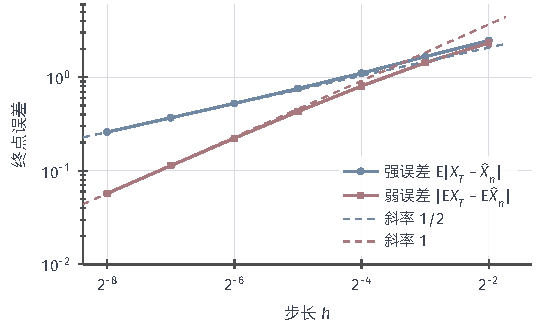
\includegraphics[width=95mm]{figures/03-optimization-evolution-and-signals/02-processes-and-trajectory-evolution/tikz/ctsp-em-orders/figure.pdf}
  \caption{Euler--Maruyama方法的终点误差，双对数刻度。模型为几何Brownian运动$\mathrm dX=2X\,\mathrm dt+X\,\mathrm dW$，$X_0=1$，$T=1$。蓝点为强误差$\mathbb E|X_T-\widehat X_n|$，由$4000$条Brownian路径（固定随机种子）在最细网格上生成增量、再合并到各粗网格，与显式解在同一路径上比较；红点为$\varphi(x)=x$的弱误差，取精确值$|e^{2}-(1+2h)^{1/h}|$。虚线是斜率$\frac12$与$1$的参考线。}
  \label{fig:ctsp-em-orders}
\end{figure}

弱误差小并不说明路径接近。设$\bm X'$是与$\bm X$独立同分布的另一份副本，则对一切可积的$\varphi$，弱误差为零，而$\mathbb E\|\bm X_T-\bm X'_T\|_2^2=2\operatorname{tr}\operatorname{Cov}(\bm X_T)$并不小。两种误差衡量的是不同的事情：强误差要求“同一噪声下走到同一个地方”，弱误差只要求“走到各处的概率一样”。

\paragraph{弱误差的望远镜机制}
弱误差为什么比强误差高阶？答案来自第~\ref{sec:ctsp-backward-forward}节的后向方程。令$u(t,\bm x)=\mathbb E[\varphi(\bm X_T)\mid\bm X_t=\bm x]$，它满足$\partial_tu+\mathcal Lu=0$、$u(T,\cdot)=\varphi$。于是
\[
  \mathbb E\varphi(\widehat{\bm X}_n)-\mathbb E\varphi(\bm X_T)=\sum_{k=0}^{n-1}\mathbb E\bigl[u(t_{k+1},\widehat{\bm X}_{k+1})-u(t_k,\widehat{\bm X}_k)\bigr],
\]
因为右端望远镜相消后剩下$\mathbb Eu(T,\widehat{\bm X}_n)-u(0,\bm X_0)$。对每一项，从$\widehat{\bm X}_k$出发，精确转移使$u$的期望保持不变；数值的一步转移与精确转移的前两阶矩只相差$O(h^2)$，在$u$有界的高阶导数下，每一项是$O(h^2)$。共$n=T/h$项，累计为$O(h)$。强误差没有这种抵消：每一步的路径误差是$O(h)$量级的随机量，其均方的累计按随机游走方式增长，得到$O(h^{1/2})$。

\paragraph{时间离散误差与Monte Carlo误差}
实际计算期望$\mathbb E\varphi(\bm X_T)$时，用$M$条独立的数值路径求平均，误差有两个来源：
\[
  \mathbb E\Bigl(\frac1M\sum_{i=1}^M\varphi(\widehat{\bm X}^{(i)}_n)-\mathbb E\varphi(\bm X_T)\Bigr)^2=\underbrace{\bigl(\mathbb E\varphi(\widehat{\bm X}_n)-\mathbb E\varphi(\bm X_T)\bigr)^2}_{\text{离散偏差}^2}+\underbrace{\frac{\operatorname{Var}\varphi(\widehat{\bm X}_n)}M}_{\text{抽样方差}} .
\]
弱一阶时偏差约为$Ch$，计算量约为$M/h$。要使均方根误差达到$\varepsilon$，需要$h\sim\varepsilon$、$M\sim\varepsilon^{-2}$，总计算量约为$\varepsilon^{-3}$。减小步长与增加路径数各自只能压低一项，应当按两项的平衡分配预算。

\paragraph{长期偏差}
上述误差界中的常数$C_T$一般随$T$增长，有限时段的收敛不能直接推出长期行为的近似：$h\to0$与$T\to\infty$两个极限不能随意交换。OU过程的例子很清楚。数值链的稳态方差$\sigma^2/[\lambda(2-\lambda h)]$与真值$\sigma^2/(2\lambda)$相差的比例为$\lambda h/(2-\lambda h)$，这个偏差不随运行时间增长而消失；步长超过$2/\lambda$时数值链甚至发散，而连续模型对任何初值都稳定。数值链的不变分布是否存在、偏离真实不变分布多少，需要单独分析。下一节用数值链做采样时，这个偏差将成为必须处理的问题。

\section{连续过程的采样与积分计算}
\label{sec:ctsp-sampling}

第~\ref{chap:discrete-time-stochastic-processes}章用离散随机序列计算积分$I=\int f\,\mathrm d\pi$：独立样本的平均，或者一条以$\pi$为不变分布的Markov链的样本平均。本节把同样的思路放到连续时间中。先说明连续时间过程怎样“求平均”，即按停留时间累计；再设计一个以给定目标为不变分布的扩散，并把它离散成可以执行的算法；最后作为补充，说明连续路径之间的似然比怎样用于重加权。

这里有两种“积分”需要分清。本节的目标是数值积分$\int f\,\mathrm d\pi$，所用的工具是沿时间的累计$\int_0^Tf(X_t)\,\mathrm dt$；第~\ref{sec:ctsp-stochastic-integration}节的Itô积分$\int H\,\mathrm dW$则是对随机驱动的累计，它出现在过程的构造与分析中，不是这里要计算的量。

\subsection{占据时间与连续时间平均}
\label{sec:ctsp-occupation}

\paragraph{从样本平均到时间平均}
离散链用$n^{-1}\sum_{k<n}f(X_k)$估计$\int f\,\mathrm d\pi$。连续时间过程没有“第$k$个样本”，相应的估计量是式~\eqref{eq:ctsp-time-average}的时间平均$\bar f_T=T^{-1}\int_0^Tf(X_t)\,\mathrm dt$。它也可以写成对\term{占据测度}（occupation measure）的积分：$L_T(A)=T^{-1}\int_0^T\mathbb I\{X_t\in A\}\,\mathrm dt$是过程在$[0,T]$内停留于$A$的时间比例，$\bar f_T=\int f\,\mathrm dL_T$。第~\ref{sec:ctsp-time-average}节的遍历定理给出这一估计量的极限：在不变分布为$\pi$且相应回返条件成立时，$L_T$弱收敛到$\pi$，$\bar f_T\to\int f\,\mathrm d\pi$。若过程不从$\pi$出发，还需检查它确实被吸引到$\pi$，并且$f$在路径上可积。

\paragraph{跳跃链的按时加权}
对连续时间Markov链，时间积分可以逐段精确计算。设链依次访问状态$Y_0,Y_1,\ldots$，各段停留时间为$S_0,S_1,\ldots$，则
\[
  \int_0^Tf(X_t)\,\mathrm dt=\sum_kf(Y_k)\,S_k ,
\]
其中最后一段截断到$T$。每次访问的贡献按停留时间加权，而不是每次跳跃记一次。

两种计数方式给出不同的平均。回到示例~\ref{ex:ctsp-two-state}中$a=1,b=2$的两态链：离开状态$1$的率为$1$，离开状态$2$的率为$2$，不变分布为$\bm\pi=(2/3,1/3)$。嵌入跳链在两个状态之间严格交替，按访问次数计，它在两个状态各占一半。图~\ref{fig:ctsp-occupation-embedded}在同一条路径上比较了两种比例：按时间累计的比例趋于$2/3$，按访问计数的比例趋于$1/2$。状态$1$的平均停留时间是状态$2$的两倍，按时间累计时它的权重也是两倍。

\begin{figure}[htbp]
  \centering
  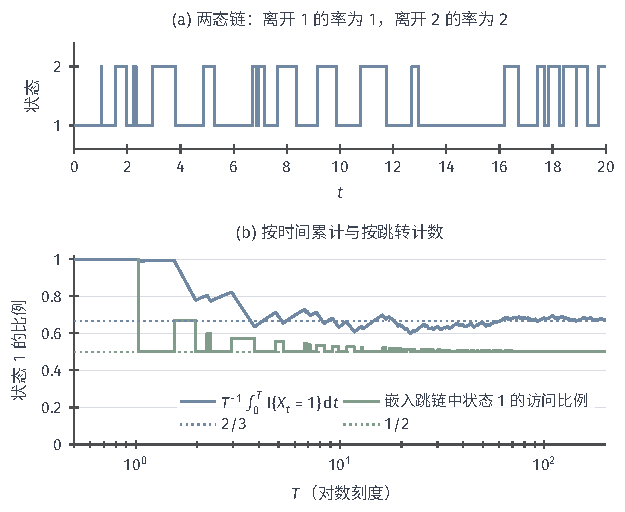
\includegraphics[width=105mm]{figures/03-optimization-evolution-and-signals/02-processes-and-trajectory-evolution/tikz/ctsp-occupation-embedded/figure.pdf}
  \caption{按时间累计与按跳转计数。两态链离开状态$1$的率为$1$，离开状态$2$的率为$2$，从状态$1$出发，固定随机种子。(a)前$20$个时间单位的路径，状态$1$的停留段平均更长；(b)同一路径上，状态$1$的占据时间比例（蓝）趋于不变分布中的$2/3$，嵌入跳链中访问状态$1$的比例（绿）趋于$1/2$，横轴为对数刻度。}
  \label{fig:ctsp-occupation-embedded}
\end{figure}

一般地，若嵌入跳链有不变分布$\bm\nu$，连续时间链的不变分布满足$\pi_i\propto\nu_i/q_i$：访问频率乘以每次访问的平均停留时间$1/q_i$。两态例中$\bm\nu=(\frac12,\frac12)$，$\bm q=(1,2)$，$\nu_i/q_i=(\frac12,\frac14)$，归一化即得$(\frac23,\frac13)$。这个关系也提示一个改进：若只想估计$\int f\,\mathrm d\pi$，可以把随机的停留时间$S_k$换成它的条件期望$1/q_{Y_k}$，估计量$\sum_kf(Y_k)/q_{Y_k}\big/\sum_k1/q_{Y_k}$消去了停留时间的随机性，这是第~\ref{chap:discrete-time-stochastic-processes}章Rao--Blackwell化的又一个实例。

\paragraph{观测方式、相关性与标准误}
实际计算中有两种累计方式。事件驱动的方式按上式精确累计，计算量与跳跃次数成正比；等间隔观察的方式只记录$X_{kh}$，用$n^{-1}\sum_kf(X_{kh})$近似，它估计的是骨架链的平均，只有在骨架链遍历时才指向$\pi$（第~\ref{sec:ctsp-time-average}节）。$h$越小，相邻观测越相关，额外的观测带来的信息越少；$h$越大，单次观测越独立，但可能错过短暂的停留。

估计误差需要长期方差。在中心极限定理成立的条件下，$\bar f_T$的标准误约为$\sigma_f/\sqrt T$，其中$\sigma_f^2=2\int_0^\infty C(s)\,\mathrm ds$是第~\ref{sec:ctsp-time-average}节的长期方差。把运行时间分成若干等长的批次，用批次平均之间的离散程度估计$\sigma_f^2$，是常用的做法；它只在批次长度远大于相关时间、并且中心极限定理适用时才可靠。遍历定理本身不提供这样的误差估计。

\subsection{以目标分布为不变分布的扩散}
\label{sec:ctsp-langevin}

\paragraph{Langevin扩散}
设目标密度$\pi(\bm x)\propto e^{-U(\bm x)}$，$U$称为势函数，只需知道到相差一个常数为止。我们希望构造一个扩散，使$\pi$是它的不变分布。直观的设计是：漂移沿$-\nabla U$把状态推向高密度区域，噪声防止它停在最低点上，二者的强度匹配到恰好保持$\pi$。这就是\term{Langevin扩散}（Langevin diffusion）
\begin{equation}
  \mathrm d\bm X_t=-\nabla U(\bm X_t)\,\mathrm dt+\sqrt2\,\mathrm d\bm W_t ,
  \label{eq:ctsp-langevin}
\end{equation}
其生成元为$\mathcal Lf=\Delta f-\nabla U^\top\nabla f$。

为什么系数是$\sqrt2$，可以由生成元的一个恒等式看出。直接展开可得$e^{-U}\mathcal Lf=\nabla\cdot(e^{-U}\nabla f)$。对$f\in C^2_c$积分，散度定理给出
\[
  \int\mathcal Lf\,\mathrm d\pi=0,\qquad
  \int g\,\mathcal Lf\,\mathrm d\pi=-\int\nabla g^\top\nabla f\,\mathrm d\pi .
\]
第一式说明$\pi$满足第~\ref{sec:ctsp-invariant}节的生成元平衡条件；第二式关于$f,g$对称，说明以$\pi$启动的过程在时间反转下规律不变，即可逆。若把噪声换成$\sigma\,\mathrm d\bm W$，平衡的密度会变成$e^{-2U/\sigma^2}$，只有$\sigma=\sqrt2$时才恰好是目标。另一种常见的写法$\mathrm d\bm Y=\frac12\nabla\log\pi(\bm Y)\,\mathrm dt+\mathrm d\bm W$描述的是同一过程放慢一半的版本：令$\bm Y_s=\bm X_{s/2}$，由Brownian尺度变换即得此式，所以两者的不变分布相同。

生成元平衡只是候选验证。要把$\pi$确认为不变分布，还需$U\in C^2$、$e^{-U}$可积，以及过程不爆炸（例如$U$在无穷远处增长，使第~\ref{sec:ctsp-sde-existence}节的Lyapunov条件成立）。唯一性与收敛需要额外的论证。噪声非退化使过程可以到达任何区域，这排除了多个不变分布；收敛速度则由下面的不等式控制。

\begin{theorem}[Poincaré不等式与方差衰减]
  \label{thm:ctsp-poincare}
  设Langevin扩散良定，$\pi$为其不变分布，并且$\pi$满足\term{Poincaré不等式}（Poincaré inequality）：存在$C_{\mathrm P}>0$，使对足够光滑的$f$，
  \[
    \operatorname{Var}_\pi(f)\leq C_{\mathrm P}\int\|\nabla f\|_2^2\,\mathrm d\pi .
  \]
  则对$\pi$平方可积的$f$，$\operatorname{Var}_\pi(P_tf)\leq e^{-2t/C_{\mathrm P}}\operatorname{Var}_\pi(f)$。
\end{theorem}

\begin{proof}
不妨设$\int f\,\mathrm d\pi=0$，则$\int P_tf\,\mathrm d\pi=0$。对足够光滑的$f$，由Kolmogorov方程与上面的对称恒等式，
\[
  \begin{aligned}
    \frac{\mathrm d}{\mathrm dt}\int(P_tf)^2\,\mathrm d\pi&=2\int P_tf\,\mathcal LP_tf\,\mathrm d\pi=-2\int\|\nabla P_tf\|_2^2\,\mathrm d\pi\\
    &\leq-\frac2{C_{\mathrm P}}\int(P_tf)^2\,\mathrm d\pi .
  \end{aligned}
\]
Grönwall不等式给出结论；一般的平方可积$f$由逼近得到，所需的定义域细节见Kallenberg的教材。
\end{proof}

定义域方面的细节可参考文献\scite{math-kallenberg2021probability}。

定理说明，从任何初值分布出发，读数$f$的条件平均以速率$1/C_{\mathrm P}$趋于其$\pi$平均。$U$强凸，即$\nabla^2U\succeq\kappa\bm I$（$\kappa>0$）时，$C_{\mathrm P}\leq1/\kappa$；多峰目标的Poincaré常数则可能很大。

\paragraph{二次势：可解的检验}
取$U(\bm x)=\frac12\bm x^\top\bm\Sigma^{-1}\bm x$，目标为$\mathcal N(\bm0,\bm\Sigma)$。式~\eqref{eq:ctsp-langevin}化为线性方程$\mathrm d\bm X=-\bm\Sigma^{-1}\bm X\,\mathrm dt+\sqrt2\,\mathrm d\bm W$，由第~\ref{sec:ctsp-linear-sde}节，稳态协方差$\bm P$解Lyapunov方程$-\bm\Sigma^{-1}\bm P-\bm P\bm\Sigma^{-1}+2\bm I=\bm0$，其解正是$\bm P=\bm\Sigma$。在$\bm\Sigma$的特征方向上，过程分解为独立的OU过程，沿特征值为$s$的方向，相关性按$e^{-t/s}$衰减。最慢的方向对应$\bm\Sigma$的最大特征值，这也是此时的Poincaré常数$C_{\mathrm P}=\lambda_{\max}(\bm\Sigma)$。

这个例子说明了混合的代价来自哪里：目标在某个方向上越宽，过程沿该方向扩散得越慢。时间平均的长期方差可以按第~\ref{sec:ctsp-time-average}节计算：沿特征值为$s$的方向，$f(\bm x)$取该方向坐标时，$\sigma_f^2=2\int_0^\infty se^{-t/s}\,\mathrm dt=2s^2$。

\paragraph{多峰与缓慢混合}
平衡等式对多峰目标同样成立，但它只保证从$\pi$出发不会离开$\pi$，不保证从别处出发能很快到达$\pi$。考虑$U(x)=2(x^2-1)^2$，目标在$x=\pm1$处有两个峰，中间$x=0$处的密度只有峰值的$e^{-2}\approx0.135$倍。过程在一个峰附近停留很久，必须依靠一串方向一致的噪声才能翻过中间的低密度区域。图~\ref{fig:ctsp-langevin-double-well}画出了一条路径和它的时间直方图：路径在两个峰之间偶尔切换，长时间运行后直方图接近目标密度，但两峰的相对权重要靠足够多次切换才能估计准确。势垒越高，切换越罕见，所需的运行时间按指数增长。

\begin{figure}[htbp]
  \centering
  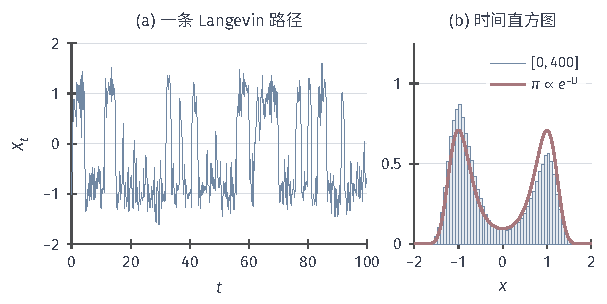
\includegraphics[width=105mm]{figures/03-optimization-evolution-and-signals/02-processes-and-trajectory-evolution/tikz/ctsp-langevin-double-well/figure.pdf}
  \caption{双峰目标上的Langevin路径。$U(x)=2(x^2-1)^2$，目标$\pi\propto e^{-U}$，用步长$2\times10^{-3}$的Euler--Maruyama离散（即下文的ULA）从$x=-1$模拟到$T=400$，固定随机种子。(a)前$100$个时间单位的路径，状态在$\pm1$附近停留并偶尔切换；(b)全部步的时间直方图与目标密度（红线）。小步长下离散偏差很小，直方图与目标的差主要来自切换次数有限。}
  \label{fig:ctsp-langevin-double-well}
\end{figure}

\subsection{连续采样的离散实现}
\label{sec:ctsp-ula-mala}

\paragraph{未校正Langevin算法}
连续扩散不能直接在计算机上运行。用Euler--Maruyama离散式~\eqref{eq:ctsp-langevin}，得到\term{未校正Langevin算法}（unadjusted Langevin algorithm，ULA）
\begin{equation}
  \bm X_{k+1}=\bm X_k-h\nabla U(\bm X_k)+\sqrt{2h}\,\bm\xi_k,\qquad\bm\xi_k\sim\mathcal N(\bm0,\bm I).
  \label{eq:ctsp-ula}
\end{equation}
每一步需要一次梯度求值和一组高斯数，不需要计算$\pi$的归一化常数。

ULA的误差有三个来源，应分别看待。第一是有限时间的路径误差，由第~\ref{sec:ctsp-error-types}节控制，在有限时段上随$h\to0$消失。第二是不变分布的偏差：数值链的长期分布不是$\pi$。第三是有限运行时间带来的初值遗留与抽样误差，由混合速度和长期方差决定。第二项不随运行时间的增加而消失。

一维标准高斯目标可以算出这个偏差。$U(x)=x^2/2$时，ULA为$X_{k+1}=(1-h)X_k+\sqrt{2h}\,\xi_k$，只有在$0<h<2$时稳定，其稳态方差为
\[
  \frac{2h}{1-(1-h)^2}=\frac1{1-h/2},
\]
而目标方差为$1$。$h=0.2$时偏高约$11\%$，$h=1$时偏高一倍。连续模型对任何初值都收敛，数值链却在$h\geq2$时发散：离散稳定性必须单独检查。对二次势$U=\frac12\bm x^\top\bm\Sigma^{-1}\bm x$，稳定要求$h<2\lambda_{\min}(\bm\Sigma)$，而最慢方向的松弛需要约$\lambda_{\max}(\bm\Sigma)/h$步；两者合起来，所需步数至少与条件数$\lambda_{\max}/\lambda_{\min}$成正比。

\paragraph{Metropolis调整的Langevin算法}
消除不变分布偏差的办法，是把ULA的一步当作提议，再用第~\ref{chap:discrete-time-stochastic-processes}章的Metropolis--Hastings规则决定是否接受。从$\bm x$出发的提议分布为
\[
  q(\bm x,\bm y)\propto\exp\Bigl\{-\frac{\|\bm y-\bm x+h\nabla U(\bm x)\|_2^2}{4h}\Bigr\},
\]
即均值$\bm x-h\nabla U(\bm x)$、协方差$2h\bm I$的高斯分布。它不对称，接受概率必须包含反向提议密度：
\begin{equation}
  \alpha(\bm x,\bm y)=\min\Bigl\{1,\frac{\pi(\bm y)\,q(\bm y,\bm x)}{\pi(\bm x)\,q(\bm x,\bm y)}\Bigr\},
  \label{eq:ctsp-mala}
\end{equation}
被拒绝时留在$\bm x$。这称为\term{Metropolis调整的Langevin算法}（Metropolis-adjusted Langevin algorithm，MALA）。由Metropolis--Hastings的细致平衡，$\pi$对任何$h>0$都是精确的不变分布。计算反向密度$q(\bm y,\bm x)$需要$\nabla U(\bm y)$，若提议被接受，这个梯度在下一步可以复用，所以每步的主要代价仍是一次梯度和一次势函数求值。

图~\ref{fig:ctsp-ula-mala}比较了两种算法。ULA的长期方差随步长偏离$1$，模拟值紧贴理论曲线$1/(1-h/2)$；MALA在所有步长下都停在$1$附近。代价体现在接受率上：步长增大时，提议越来越大胆，被拒绝得越来越多，链停在原地的时间变长，有效样本随之减少。接受校正消除的是偏差，不是相关性。

\begin{figure}[htbp]
  \centering
  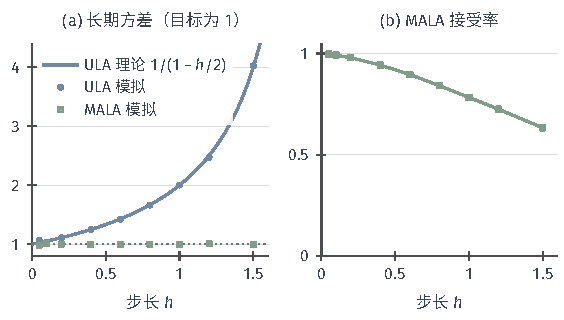
\includegraphics[width=96mm]{figures/03-optimization-evolution-and-signals/02-processes-and-trajectory-evolution/tikz/ctsp-ula-mala/figure.pdf}
  \caption{标准高斯目标上的ULA与MALA。每个步长$h$各运行$1.2\times10^5$步，从$0$出发，固定随机种子。(a)$X^2$的时间平均，即长期方差的估计：ULA（蓝点）沿理论曲线$1/(1-h/2)$偏离目标值$1$，MALA（绿点）保持在$1$附近；(b)MALA的平均接受率随步长下降。}
  \label{fig:ctsp-ula-mala}
\end{figure}

ULA与MALA本身都是离散时间的Markov链，它们的遍历性与误差分析属于第~\ref{chap:discrete-time-stochastic-processes}章的框架。把它们放在这里，是为了说明一个连续时间模型怎样变成可以执行的采样方法：连续扩散提供“往哪里走、走多远”的设计，离散化提供计算步骤，接受校正修复离散化引入的偏差。

\subsection{连续路径换测度（补充）}
\label{sec:ctsp-girsanov}

\paragraph{从有限路径的似然比出发}
第~\ref{chap:discrete-time-stochastic-processes}章的路径重加权把有限路径在两个模型下的密度之比写成各步条件密度之比的连乘。对连续时间扩散，可以先在网格上写出这个比值，再看网格加细时会发生什么。设两个模型$\mathrm dX=\beta(X)\,\mathrm dt+\mathrm dW$与$\mathrm dX=\mathrm dW$，在步长$h$的Euler离散下，一步转移密度之比为
\[
  \frac{\exp\{-(\Delta X-\beta h)^2/(2h)\}}{\exp\{-(\Delta X)^2/(2h)\}}=\exp\Bigl\{\beta\,\Delta X-\frac12\beta^2h\Bigr\}.
\]
连乘以后，指数是$\sum\beta(X_{t_k})\Delta X_k-\frac12\sum\beta(X_{t_k})^2h$，网格加细时它趋于$\int_0^T\beta\,\mathrm dX-\frac12\int_0^T\beta^2\,\mathrm dt$。分母中的$h$恰好相消，这是两个模型扩散系数相同的结果。若扩散系数不同，每一步的比值都带有一个与$h$有关的常数因子，连乘后发散或趋零，极限不存在。所以连续路径的似然比不能无条件地由离散连乘取极限得到，需要单独的定理。

\paragraph{随机指数与Novikov条件}
设$\bm\theta$是$\mathbb R^m$值的可预测过程，$\int_0^T\|\bm\theta_s\|_2^2\,\mathrm ds<\infty$几乎必然，定义
\begin{equation}
  Z_t=\exp\Bigl\{\int_0^t\bm\theta_s^\top\mathrm d\bm W_s-\frac12\int_0^t\|\bm\theta_s\|_2^2\,\mathrm ds\Bigr\},
  \label{eq:ctsp-stochastic-exponential}
\end{equation}
称为\term{随机指数}（stochastic exponential）。由Itô公式，$\mathrm dZ_t=Z_t\bm\theta_t^\top\mathrm d\bm W_t$，漂移恰好消失，所以$Z$是正的局部鞅，由第~\ref{sec:ctsp-continuous-martingales}节它是超鞅，$\mathbb EZ_T\leq1$。$Z$能否作为密度，取决于$\mathbb EZ_T=1$是否成立，即$Z$是否为真鞅。一个常用的充分条件是\term{Novikov条件}（Novikov condition）
\begin{equation}
  \mathbb E\exp\Bigl\{\frac12\int_0^T\|\bm\theta_s\|_2^2\,\mathrm ds\Bigr\}<\infty ,
  \label{eq:ctsp-novikov}
\end{equation}
其证明见Øksendal的教材\scite{math-oksendal2003sde}。若$\|\bm\theta\|_2\leq c$，被积指数不超过$c^2T/2$，条件自然成立。

\paragraph{Girsanov定理}
当$Z$是真鞅时，可以用它定义新的概率测度，并精确描述Brownian运动在新测度下的样子。换测度的一般框架，即用非负、期望为一的随机变量作为Radon--Nikodym密度定义新测度，见\BookChapterRef{chap:densities-change-of-measure}{卷二“密度与换测度”章}。

\begin{theorem}[Girsanov定理]
  \label{thm:ctsp-girsanov}
  设$Z$由式~\eqref{eq:ctsp-stochastic-exponential}定义且$\mathbb EZ_T=1$。令$\mathrm d\mathbb Q=Z_T\,\mathrm d\mathbb P$于$\mathcal F_T$。则在$\mathbb Q$下，
  \[
    \widetilde{\bm W}_t=\bm W_t-\int_0^t\bm\theta_s\,\mathrm ds,\qquad0\leq t\leq T,
  \]
  是标准Brownian运动。
\end{theorem}

定理~\ref{thm:ctsp-girsanov}称为\term{Girsanov定理}（Girsanov theorem）。它的证明需要Lévy的Brownian刻画（连续局部鞅、二次变差为$t$即为Brownian运动），这里只解释它的含义\scite{math-kallenberg2021probability}。在原测度下，$\bm W$没有漂移；换到$\mathbb Q$以后，$\bm W$获得漂移$\bm\theta$，而扣掉这一漂移的$\widetilde{\bm W}$成为新的Brownian运动。换测度只改变漂移，不改变二次变差：二次变差是沿路径加细分割得到的极限，在一个测度下几乎必然成立的事，在与之等价的测度下也几乎必然成立。

应用于扩散，设$\mathrm d\bm X=\bm b(\bm X)\,\mathrm dt+\bm\sigma\,\mathrm d\bm W$在$\mathbb P$下成立，$\bm\sigma$可逆。取$\bm\theta=\bm\sigma^{-1}(\bm b'-\bm b)(\bm X)$，则在$\mathbb Q$下$\mathrm d\bm X=\bm b'(\bm X)\,\mathrm dt+\bm\sigma\,\mathrm d\widetilde{\bm W}$。于是任何路径泛函$F$满足
\[
  \mathbb E_{\mathbb Q}F(\bm X_{[0,T]})=\mathbb E_{\mathbb P}\bigl[Z_TF(\bm X_{[0,T]})\bigr]:
\]
可以在一个模型下模拟路径，乘以权重$Z_T$，估计另一个模型下的期望。这是有限路径重加权的连续时间版本。

\begin{example}[用漂移估计罕见事件]
  \label{ex:ctsp-girsanov-rare-event}
  估计$p=\mathbb P(W_1>4)=1-\Phi(4)\approx3.17\times10^{-5}$。直接模拟时，每$31574$个样本平均只有一个落入事件，相对方差$(1-p)/p\approx3.16\times10^4$，要使相对误差降到$10\%$约需$3.2\times10^6$个样本。改在常数漂移$\theta=4$下模拟，即$W_1\sim\mathcal N(4,1)$，并乘以权重$\exp\{-4W_1+8\}$（$Z_1^{-1}$），估计量的二阶矩为$e^{16}[1-\Phi(8)]\approx5.53\times10^{-9}$，相对方差约为$4.5$，同样的精度只需约$450$个样本。漂移把路径推向罕见事件发生的区域，权重则精确地抵消了这一推动。
\end{example}

\paragraph{需要分别核对的条件}
例子中的方差缩减并不是一般规律。权重是合法密度（$\mathbb EZ_T=1$）与权重的二阶矩有限是两个不同的条件：前者保证估计量无偏，后者保证估计量的方差有限。漂移差很大或时域很长时，$Z_T$可能高度偏斜，少数路径携带几乎全部权重，这与离散长路径的权重退化是同一现象。

两个扩散系数不同的模型，其路径规律一般相互奇异，没有密度可言。以$W$与$2W$为例，在$[0,T]$上前者的二次变差为$T$，后者为$4T$；事件“二次变差等于$T$”在一个模型下概率为一，在另一个模型下概率为零。所以连续路径的换测度只能改变漂移，不能当然地改变扩散系数。基于路径权重评价行动策略属于后续的决策与控制部分，依据观测对路径重加权属于第~\ref{chap:state-space-estimation}章，这里只建立路径权重的概率关系。

\section{应用：连续时间随机逼近}
\label{sec:ctsp-stochastic-approximation}

上一节的采样过程要长期保持一个非退化的分布：噪声不能消失，否则过程会停在势函数的最低点，而不是遍历整个目标。本节的任务相反。第~\ref{chap:discrete-time-stochastic-processes}章的Robbins--Monro递推只能观察到带噪声的响应，却要逼近方程$h(\bm\theta)=\bm0$的根；它让步长逐渐减小，使噪声的影响越来越弱，最终把迭代钉在根上。这里把这个机制放到连续时间：观测是连续到达的带噪信号，增益随时间递减，问题是状态是否收敛到指定的零点。

\subsection{连续观测与递减增益}
\label{sec:ctsp-sa-setting}

\paragraph{从离散递推到连续观测}
离散的随机逼近写成$\bm\theta_{n+1}=\bm\theta_n+a_n[h(\bm\theta_n)+\bm\xi_{n+1}]$：平均漂移$h$把迭代推向根，鞅差$\bm\xi_{n+1}$是观测噪声，步长$a_n$满足$\sum a_n=\infty$、$\sum a_n^2<\infty$。连续时间中，带噪响应以信号的形式到达：设观测过程满足
\begin{equation}
  \mathrm d\bm Y_t=h(\bm\theta_t)\,\mathrm dt+\bm\sigma(\bm\theta_t)\,\mathrm d\bm W_t ,
  \label{eq:ctsp-sa-observation}
\end{equation}
每段短时间内观测到的增量$\mathrm d\bm Y_t$是当前参数下平均响应的$\mathrm dt$倍，叠加一个Brownian噪声。增益为$a(t)>0$的连续随机逼近按观测调整参数：
\begin{equation}
  \mathrm d\bm\theta_t=a(t)\,\mathrm d\bm Y_t=a(t)h(\bm\theta_t)\,\mathrm dt+a(t)\bm\sigma(\bm\theta_t)\,\mathrm d\bm W_t .
  \label{eq:ctsp-continuous-sa}
\end{equation}
与离散情形一样，算法使用的是观测$\mathrm d\bm Y$，并不需要能直接计算$h$；$h$与$\bm\sigma$只在分析中出现。

\paragraph{增益条件的含义}
本节取确定的、连续的正增益$a(t)$，常用的例子是$a(t)=1/(1+t)$。离散步长的两个条件在连续时间中对应
\begin{equation}
  \int_0^\infty a(t)\,\mathrm dt=\infty,\qquad\int_0^\infty a(t)^2\,\mathrm dt<\infty .
  \label{eq:ctsp-gain-conditions}
\end{equation}
第一个条件保留累计调整能力：确定性部分$\dot{\bm\theta}=a(t)h(\bm\theta)$走过的“路程”由$\int a\,\mathrm dt$度量，它必须是无穷，才能从任意远的初值走到根。第二个条件控制噪声：在$\bm\sigma$有界时，噪声项$\int_0^ta(s)\bm\sigma\,\mathrm d\bm W_s$的二阶矩由Itô等距等于$\int_0^ta^2\|\bm\sigma\|_{\mathrm F}^2\,\mathrm ds$，有限的总量使这个鞅$L^2$有界，从而收敛，噪声的总影响有限。$a(t)=1/(1+t)$同时满足两者；$a(t)=(1+t)^{-\beta}$在$\frac12<\beta\leq1$时满足，$\beta\leq\frac12$时噪声累计无界，$\beta>1$时调整总量有限。

增益条件只是收敛的一部分条件。还需要方程~\eqref{eq:ctsp-continuous-sa}有不爆炸的解，噪声的矩受控，并且平均漂移$h$确实把状态吸引向根。下一小节在一组可以直接检查的条件下把这些部分组合起来。

\subsection{随机Lyapunov方法与平均动力学}
\label{sec:ctsp-sa-lyapunov}

\paragraph{收敛定理}
离散章用非负误差量的几乎超鞅递推证明随机逼近收敛。连续时间的对应工具是：对误差的Lyapunov函数使用Itô公式，把漂移的下降、二阶修正和鞅项分开，再把正的二阶修正吸收进一个积分因子。

\begin{theorem}[连续时间随机逼近的收敛]
  \label{thm:ctsp-sa-convergence}
  设$h$与$\bm\sigma$全局Lipschitz，$\bm\theta^\star$满足$h(\bm\theta^\star)=\bm0$，并且存在常数$c,K>0$，使对所有$\bm\theta$，
  \[
    (\bm\theta-\bm\theta^\star)^\top h(\bm\theta)\leq-c\|\bm\theta-\bm\theta^\star\|_2^2,\qquad
    \|\bm\sigma(\bm\theta)\|_{\mathrm F}^2\leq K\bigl(1+\|\bm\theta-\bm\theta^\star\|_2^2\bigr).
  \]
  设增益$a(t)$确定、连续、为正并满足式~\eqref{eq:ctsp-gain-conditions}，初值$\bm\theta_0$确定。则$\bm\theta_t\to\bm\theta^\star$几乎必然。
\end{theorem}

\begin{proof}
系数全局Lipschitz（乘以局部有界的$a(t)$后在有限时段上仍是），定理~\ref{thm:ctsp-sde-existence}给出全时间的强解。记$V_t=\|\bm\theta_t-\bm\theta^\star\|_2^2$。由Itô公式，
\[
  \mathrm dV_t=\bigl[2a(t)(\bm\theta_t-\bm\theta^\star)^\top h(\bm\theta_t)+a(t)^2\|\bm\sigma(\bm\theta_t)\|_{\mathrm F}^2\bigr]\mathrm dt+\mathrm dM_t ,
\]
其中$M_t=\int_0^t2a(s)(\bm\theta_s-\bm\theta^\star)^\top\bm\sigma(\bm\theta_s)\,\mathrm d\bm W_s$是局部鞅。由两个假设，漂移不超过$-2caV_t+Ka^2(1+V_t)$。

正的二阶修正$Ka^2(1+V)$用积分因子吸收。令
\[
  A_t=\exp\Bigl\{-K\int_0^ta(s)^2\,\mathrm ds\Bigr\},
\]
由增益条件，$A_t$从$1$单调下降到正的极限$A_\infty$。由乘积法则（$A$有限变差），
\[
  \mathrm d\bigl[A_t(1+V_t)\bigr]=A_t\bigl[\mathrm dV_t-Ka(t)^2(1+V_t)\,\mathrm dt\bigr]\leq-2ca(t)A_tV_t\,\mathrm dt+A_t\,\mathrm dM_t .
\]
于是$S_t=A_t(1+V_t)+\int_0^t2ca(s)A_sV_s\,\mathrm ds$满足$\mathrm dS_t\leq A_t\,\mathrm dM_t$。记$L_t=S_0+\int_0^tA_s\,\mathrm dM_s$，则$L_t-S_t$非减且从零出发，所以$0\leq S_t\leq L_t$。$L$是非负局部鞅，由第~\ref{sec:ctsp-continuous-martingales}节它是超鞅；对$s\leq t$，$\mathbb E[S_t\mid\mathcal F_s]=\mathbb E[L_t\mid\mathcal F_s]-\mathbb E[L_t-S_t\mid\mathcal F_s]\leq L_s-(L_s-S_s)=S_s$，所以$S$也是非负超鞅。由定理~\ref{thm:ctsp-martingale-convergence}，$S_t$几乎必然收敛到有限极限。

$S$的两部分都非负，第二部分随$t$非减，所以二者分别收敛：$\int_0^\infty a(s)A_sV_s\,\mathrm ds<\infty$，并且$A_t(1+V_t)$收敛，再由$A_t\to A_\infty>0$得$V_t$收敛到某个$V_\infty$。若$V_\infty>0$，由$A_s\geq A_\infty$，积分$\int_0^\infty a(s)A_sV_s\,\mathrm ds$的被积函数最终不小于$\frac12a(s)A_\infty V_\infty$，而$\int a=\infty$，矛盾。所以$V_\infty=0$。
\end{proof}

证明的结构与离散章的几乎超鞅定理一一对应：$-2caV$是累计下降项，$Ka^2(1+V)$是可求和的误差项（由$\int a^2<\infty$），$M$是鞅噪声。连续时间新增的是两步：用Itô公式而不是一步展开得到漂移，以及用局部化与Fatou引理处理只是局部鞅的噪声。强单调条件可以放宽为一般的Lyapunov函数条件，但需要另外保证轨迹有界。

\paragraph{常增益的对照}
若把增益固定为常数$a$，第二个增益条件失效，噪声不再消失。以标量$h(\theta)=\mu-\theta$、常数$\sigma$为例，式~\eqref{eq:ctsp-continuous-sa}化为$\mathrm d\theta=a(\mu-\theta)\,\mathrm dt+a\sigma\,\mathrm dW$，这是一个以$\mu$为中心的OU过程，稳态方差为$(a\sigma)^2/(2a)=a\sigma^2/2$。状态在$\mu$附近持续波动，波动幅度按$\sqrt a$缩小；它跟踪得快，但不收敛。常增益适合目标会缓慢变化的情形，此时研究的是稳态波动与跟踪误差，而不是收敛。这里的方差公式依赖噪声非退化与线性结构；一般非线性情形只能给出上界，正的极限方差需要额外条件。

\paragraph{算法时钟与平均ODE}
增益递减的过程还可以换一个时钟来看。定义算法时间$s(t)=\int_0^ta(u)\,\mathrm du$，它是严格递增的连续函数，由第一个增益条件趋于无穷；记其反函数为$t(s)$，令$\widetilde{\bm\theta}_s=\bm\theta_{t(s)}$。漂移部分在新时钟下变成$h(\widetilde{\bm\theta}_s)\,\mathrm ds$，增益被吸收掉了。噪声部分需要一个时间变换的事实：$\bm B_s=\int_0^{t(s)}\sqrt{a(u)}\,\mathrm d\bm W_u$是连续鞅，二次变差为$\int_0^{t(s)}a(u)\,\mathrm du\,\bm I=s\bm I$，由Lévy的Brownian刻画它是标准Brownian运动\scite{math-kallenberg2021probability}。由$a\,\mathrm dW=\sqrt a\cdot\sqrt a\,\mathrm dW$，
\begin{equation}
  \mathrm d\widetilde{\bm\theta}_s=h(\widetilde{\bm\theta}_s)\,\mathrm ds+\sqrt{a(t(s))}\,\bm\sigma(\widetilde{\bm\theta}_s)\,\mathrm d\bm B_s .
  \label{eq:ctsp-algorithm-clock}
\end{equation}

在算法时钟下，确定性部分就是平均ODE $\dot{\bm\theta}=h(\bm\theta)$，与离散章的平均ODE方法一致；噪声的系数是$\sqrt{a(t(s))}$，随算法时间趋于零。所以长时间以后，过程在任意固定长度的算法时间窗内越来越接近平均ODE的轨迹，收敛性可以从ODE的稳定性读出。上面的定理没有走这条路，而是直接用Lyapunov函数闭合证明，因为它只需要可以逐项检查的条件。这里的时间变换只改变给定增益下的时间尺度；它说明递减增益的随机逼近为什么可以用平均ODE描述，并不意味着所有随机微分方程都是随机逼近。

\subsection{可解实例、离散实现与误差分工}
\label{sec:ctsp-sa-example}

\paragraph{连续观测下的均值估计}
最简单的例子是估计一个未知漂移。设观测为$\mathrm dY_t=\mu\,\mathrm dt+\sigma\,\mathrm dW_t$，$Y_0=0$，目标是$\mu$。取$h(\theta)=\mu-\theta$，即用观测增量减去当前估计的预测，增益$a(t)=1/(1+t)$：
\[
  \mathrm d\theta_t=\frac{\mathrm dY_t-\theta_t\,\mathrm dt}{1+t} .
\]
乘以$1+t$并用乘积法则，$\mathrm d[(1+t)\theta_t]=\theta_t\,\mathrm dt+(1+t)\,\mathrm d\theta_t=\mathrm dY_t$，所以
\begin{equation}
  \theta_t=\frac{\theta_0+Y_t}{1+t} .
  \label{eq:ctsp-sa-solution}
\end{equation}
由$Y_t=\mu t+\sigma W_t$，
\[
  \mathbb E\theta_t=\frac{\theta_0+\mu t}{1+t}=\mu+\frac{\theta_0-\mu}{1+t},\qquad
  \operatorname{Var}(\theta_t)=\frac{\sigma^2t}{(1+t)^2}.
\]
偏差按$1/t$消失，方差按$\sigma^2/t$下降，均方误差约为$\sigma^2/t$。由$W_t/t\to0$几乎必然，$\theta_t\to\mu$几乎必然，这与定理~\ref{thm:ctsp-sa-convergence}的结论一致（这里$c=1$，$K=\sigma^2$）。图~\ref{fig:ctsp-sa-paths}画出了路径束：所有路径从同一初值出发，偏差与波动同时收缩。

\begin{figure}[htbp]
  \centering
  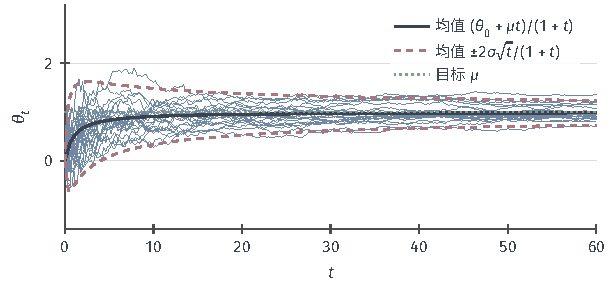
\includegraphics[width=105mm]{figures/03-optimization-evolution-and-signals/02-processes-and-trajectory-evolution/tikz/ctsp-sa-paths/figure.pdf}
  \caption{连续时间随机逼近的路径束。观测$\mathrm dY=\mu\,\mathrm dt+\sigma\,\mathrm dW$，$\mu=1$，$\sigma=1$，增益$1/(1+t)$，$\theta_0=0$；由显式解$\theta_t=(\theta_0+Y_t)/(1+t)$在网格上生成$25$条路径，固定随机种子。黑线为均值，红虚线为均值$\pm2\sigma\sqrt t/(1+t)$，绿点线为目标$\mu$。与图~\ref{fig:ctsp-ou-envelope}的OU过程不同，这里的波动带随时间收窄到零。}
  \label{fig:ctsp-sa-paths}
\end{figure}

这个例子也说明，同一个对象可以从两个角度研究。作为算法，$\theta_t$是一个随机逼近过程，我们关心它是否、以多快的速度收敛到方程的根$\mu$。作为统计量，$\theta_t\approx Y_t/t$是由连续观测估计漂移的估计量，可以继续问它在所有估计量中是否最优、渐近分布能否用来构造置信区间。前一个问题属于本节，后一个问题需要统计推断的框架，见\BookChapterRef{chap:statistical-inference}{卷四“统计推断”章}。

\paragraph{离散实现与误差分工}
在计算机上实现连续随机逼近，需要把时间离散。取步长$\Delta$，第$k$步的增益为$a_k=a(k\Delta)\Delta$，观测增量为$\Delta Y_k=Y_{(k+1)\Delta}-Y_{k\Delta}$，更新为$\theta_{k+1}=\theta_k+a(k\Delta)[\Delta Y_k-\theta_k\Delta]$。这已经是一个离散的Robbins--Monro递推，步长$a_k$满足离散的两个条件。

误差来源应当分别记录。一是增益调度的离散：$a_k$是连续增益的近似，改变了有效的算法时钟。二是时间网格：在每步内冻结$\theta$，与连续方程相差一个与$\Delta$同阶的项。三是噪声的生成：若$Y$本身是模拟的，模拟误差按第~\ref{sec:ctsp-error-types}节分析；若$Y$来自真实观测，则没有这一项。四是有限运行时间：即使离散与连续完全一致，在时刻$T$停止时仍有$\sigma^2/T$量级的随机误差。前三项属于数值计算，第四项是算法本身在有限时间内的误差。至于$\mu$能否从观测中识别、估计量是否有效，是统计问题，不在这里的误差分工之内。

\section{离散近似与过程极限（进阶）}
\label{sec:ctsp-process-limits}

本章多次借用一个直觉：步长很小的随机游走“看起来像”Brownian运动，微小增量的Markov链“看起来像”扩散。第~\ref{sec:ctsp-brownian}节用它引出$\sqrt{\Delta t}$缩放，第~\ref{sec:ctsp-numerical}节用它构造数值格式。本节说明这个直觉在什么意义下成立：不仅每个固定时刻的分布收敛，整条随机路径的分布也收敛。这比逐时刻的极限多了对整条路径的控制，因而需要额外的条件。本节是进阶内容，前两节的采样与随机逼近结论并不依赖这里的路径极限理论。

\subsection{路径距离与紧性}
\label{sec:ctsp-path-space}

\paragraph{连续路径的一致距离}
要说一列随机路径的分布收敛，先要规定两条路径怎样才算接近。对$[0,T]$上的连续实值路径，自然的距离是一致距离$\|x-y\|_\infty=\sup_{t\leq T}|x(t)-y(t)|$。连续路径空间$C([0,T])$在这一距离下完备可分，是Polish空间，因而可以使用分布弱收敛的一般理论。随机路径$X_n$的分布弱收敛到$X$，记作$X_n\Rightarrow X$，指对$C([0,T])$上每个有界连续泛函$F$，$\mathbb EF(X_n)\to\mathbb EF(X)$。

这里有两种不同的“接近”。若$X_n$与$X$定义在同一概率空间上，可以问$\|X_n-X\|_\infty$是否依概率趋零，这是第~\ref{sec:ctsp-error-types}节强误差的路径版本，需要把两者耦合起来。分布弱收敛则不要求耦合，只比较路径的规律；它是弱误差的路径版本，随机游走与Brownian运动通常生活在不同的概率空间上，能谈论的只有这一种。

\paragraph{跳跃路径与Skorokhod时间对齐}
跳跃路径不能用一致距离比较。设$x(t)=\mathbb I\{t\geq\frac12\}$，$x_n(t)=\mathbb I\{t\geq\tau_n\}$，$\tau_n\downarrow\frac12$。两条路径只是跳跃时刻略有错开，直觉上应当很接近；但在两次跳跃之间，一条已经取$1$，另一条仍取$0$，所以$\|x_n-x\|_\infty=1$对所有$n$成立。图~\ref{fig:ctsp-path-space-examples}(a)画出了这一情形。

\term{Skorokhod拓扑}（Skorokhod $J_1$ topology）允许先把时间轴轻微地拉伸或压缩，再比较取值。若存在严格递增的连续双射$\lambda_n:[0,T]\to[0,T]$，使
\[
  \|\lambda_n-\mathrm{id}\|_\infty\to0,\qquad\|x_n\circ\lambda_n-x\|_\infty\to0 ,
\]
就称$x_n$在$J_1$意义下收敛到$x$。在上面的例子中，取经过$(0,0)$、$(\frac12,\tau_n)$、$(1,1)$的分段线性$\lambda_n$，它把$x$的跳跃时刻送到$x_n$的跳跃时刻，于是$x_n\circ\lambda_n=x$，而$\|\lambda_n-\mathrm{id}\|_\infty=\tau_n-\frac12\to0$。右连续有左极限的路径空间$D([0,T])$在这一拓扑下也可以赋予完备可分的度量\scite{math-kallenberg2021probability}。若极限路径连续，$J_1$收敛与一致收敛等价。

\paragraph{有限维收敛的不足}
最直接的猜想是：只要每组有限个时刻上的联合分布收敛，路径分布就收敛。下面的确定性例子说明这不够。令
\[
  x_n(t)=\max\{1-n^2|t-1/n|,0\},\qquad t\in[0,1],\ n\geq2 ,
\]
它是一个以$1/n$为中心、高为$1$、宽为$2/n^2$的尖峰，见图~\ref{fig:ctsp-path-space-examples}(b)。固定任意时刻$t$，当$n$足够大时尖峰已经移到$t$的左侧并且宽度小于$t$，所以$x_n(t)\to0$；任意有限个时刻同时如此。可是$\|x_n\|_\infty=1$，$x_n$在$C([0,1])$中不收敛到零。越来越窄的尖峰从有限个截面之间溜过，有限维分布看不到它。

\begin{figure}[htbp]
  \centering
  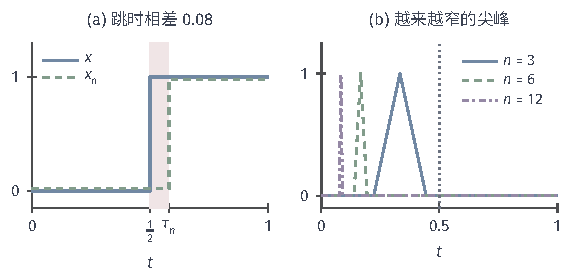
\includegraphics[width=97mm]{figures/03-optimization-evolution-and-signals/02-processes-and-trajectory-evolution/tikz/ctsp-path-space-examples/figure.pdf}
  \caption{路径空间中的两种比较（解析式教学图）。(a)跳跃时刻分别为$\frac12$与$\tau_n=0.58$的两条阶梯路径（绿线略向内偏移以便辨认），浅红带内二者相差$1$，一致距离为$1$，经时间对齐后的$J_1$距离不超过$0.08$；(b)尖峰$x_n(t)=\max\{1-n^2|t-1/n|,0\}$，$n=3,6,12$。任一固定时刻（如点线$t=\frac12$）最终只看到零，路径的最大值却始终为$1$。}
  \label{fig:ctsp-path-space-examples}
\end{figure}

\paragraph{紧性判据}
缺的是对路径整体形状的统一控制。对连续路径，这由Arzelà--Ascoli定理刻画：$C([0,T])$中的一族函数相对紧，当且仅当它们在起点处一致有界并且等度连续，即对每个误差阈值，能选同一个时间间隔同时控制族内所有函数的短时变化。把这一判据翻译成概率语言，用连续模
\[
  w(x,\delta)=\sup\{|x(t)-x(s)|:s,t\in[0,T],\ |t-s|\leq\delta\}
\]
描述短时振荡，就得到路径分布紧性的判据。

\begin{theorem}[连续路径的紧性]
  \label{thm:ctsp-tightness}
  设$X_n$是$C([0,T])$值的随机路径。若$(X_n(0))_n$的分布一致紧，并且对每个$\varepsilon>0$，
  \[
    \lim_{\delta\downarrow0}\sup_n\mathbb P\bigl(w(X_n,\delta)>\varepsilon\bigr)=0 ,
  \]
  则$(X_n)$的分布族一致紧。
\end{theorem}

\begin{proof}
固定$\eta\in(0,1)$。选$M$使$\sup_n\mathbb P(|X_n(0)|>M)\leq\eta/2$；对$k=1,2,\ldots$，选$\delta_k\downarrow0$使$\sup_n\mathbb P(w(X_n,\delta_k)>2^{-k})\leq\eta2^{-k-1}$。由联合界，每个$X_n$以至少$1-\eta$的概率落入集合$\mathcal K=\{x:|x(0)|\leq M,\ w(x,\delta_k)\leq2^{-k}\ \forall k\}$。$\mathcal K$中的函数等度连续；把$[0,T]$分成长度不超过$\delta_1$的有限段，又得到统一的幅度界。由Arzelà--Ascoli定理，$\mathcal K$的闭包是紧集。
\end{proof}

Arzelà--Ascoli定理可参考文献\scite{math-folland1999real}。

增量矩界是检验振荡条件的常用充分条件：若存在$p,\beta,C>0$，使对所有$n$与$s,t$，$\mathbb E|X_n(t)-X_n(s)|^p\leq C|t-s|^{1+\beta}$，并且初值一致紧，则振荡条件成立。这是第~\ref{chap:stochastic-processes-and-sample-paths}章Kolmogorov连续性准则的一致版本：常数对整列过程统一。

跳跃路径不能使用连续模：一次合法的跳跃就使$w(x,\delta)$无法随$\delta$趋零。$D([0,T])$中的紧性要换用其他判据，常用的是Aldous条件：路径在有界时间内以高概率停留在紧集中，并且对任意有界停时$\rho_n$与趋于零的常数$\delta_n$，$X_n(\rho_n+\delta_n)-X_n(\rho_n)\to0$依概率成立\scite{math-kallenberg2021probability}。它要求的是“在随机时刻之后的短时间内不发生大的变化”，允许跳跃但排除跳跃的聚集。两种判据针对不同的路径空间，不能混用。

\subsection{从有限维分布识别过程极限}
\label{sec:ctsp-identify-limit}

\paragraph{子列极限与识别}
紧性本身不给出极限，只保证极限点存在。证明过程收敛的标准路线分两步。第一步，由紧性与Prokhorov定理，路径分布的每个子列都有进一步的子列弱收敛；Prokhorov定理与弱收敛的一般性质见\BookChapterRef{chap:weak-convergence-limit-theorems}{卷二“弱收敛与极限定理”章}。第二步，识别这些子列极限：若有限维分布收敛到某个过程$X$的有限维分布，则每个子列极限都与$X$有相同的有限维分布。

第二步之所以可行，是因为坐标映射$x\mapsto(x(t_1),\ldots,x(t_k))$在$C([0,T])$上连续，连续映射保持弱收敛，所以子列极限的有限维分布就是有限维分布的极限；而连续路径的分布由有限维分布唯一确定（路径空间的Borel $\sigma$代数由坐标映射生成）。于是所有子列极限相同，整列收敛：
\[
  \text{紧性}+\text{有限维分布收敛}\ \Longrightarrow\ X_n\Rightarrow X\quad\text{于}C([0,T]).
\]
在$D([0,T])$中，坐标映射只在路径连续的时刻连续，所以有限维收敛只需在极限过程几乎必然不跳的时刻核对；这样的时刻在$[0,T]$中稠密，足以确定分布。

\paragraph{连续映射与路径泛函}
过程收敛的用处在于把极限传递给路径泛函。若$X_n\Rightarrow X$于$C([0,T])$，$F$是在$X$的几乎每条路径处连续的泛函，则$F(X_n)\Rightarrow F(X)$。常见的泛函需要逐个核对连续性。
\begin{itemize}
  \item 最大值$F(x)=\max_{t\leq T}x(t)$与时间积分$F(x)=\int_0^Tg(x(t))\,\mathrm dt$（$g$连续有界）在一致距离下连续，可以直接传递。
  \item 首次到达时刻$\tau_a(x)=\inf\{t:x(t)\geq a\}$不是处处连续的。设$x$在$[0,1]$上从$0$线性升到$a$，在$[1,2]$上停在$a$，之后线性上升越过$a$；则$\tau_a(x)=1$，而$x-\frac1n$直到$t=2+\frac1n$才到达$a$，所以$\tau_a(x-\frac1n)\to2\neq1$。问题出在路径“碰到$a$却没有越过”。Brownian路径到达$a$后立即越过$a$（由强Markov性质与反射原理），这种接触几乎必然不发生，所以$\tau_a$在Brownian运动的几乎每条路径处连续，可以传递。
\end{itemize}
在$D([0,T])$中，最大值仍然连续，固定时刻的取值则只在极限路径于该时刻连续时连续。

\subsection{随机游走与扩散近似}
\label{sec:ctsp-donsker}

\paragraph{Donsker定理}
现在可以准确陈述第~\ref{sec:ctsp-brownian}节的直觉。设$\xi_1,\xi_2,\ldots$独立同分布，均值为零，方差为一，$S_k=\xi_1+\cdots+\xi_k$。对每个$n$，在时刻$k/n$放置值$S_k/\sqrt n$，并在相邻时刻之间线性插值，得到$C([0,1])$中的随机折线$X_n$。

\begin{theorem}[Donsker定理]
  \label{thm:ctsp-donsker}
  在上述条件下，$X_n\Rightarrow W$于$C([0,1])$，其中$W$是标准Brownian运动。
\end{theorem}

定理~\ref{thm:ctsp-donsker}称为\term{Donsker定理}（Donsker theorem），也称函数型中心极限定理。证明沿上一小节的两步进行\scite{math-kallenberg2021probability}。有限维分布的收敛来自多元中心极限定理：对$0<t_1<\cdots<t_k$，各段增量$S_{\lfloor nt_i\rfloor}-S_{\lfloor nt_{i-1}\rfloor}$相互独立，标准化后分别趋于$\mathcal N(0,t_i-t_{i-1})$，插值的修正项依概率趋零。紧性需要控制振荡；若再假设$\mathbb E\xi_1^4<\infty$，网格点上$\mathbb E(S_k-S_j)^4\leq C(k-j)^2$，于是$\mathbb E|X_n(t)-X_n(s)|^4\leq C'|t-s|^2$，上一小节的矩判据适用（网格间的插值段需要单独但简单的估计）。只有二阶矩时，紧性需要更精细的最大不等式。图~\ref{fig:ctsp-donsker}画出了同一列$\pm1$步长在三个尺度上的缩放折线：步数增加时，折线的锯齿变细，整体的起伏幅度保持在同一量级，逐渐呈现Brownian路径的样子。

\begin{figure}[htbp]
  \centering
  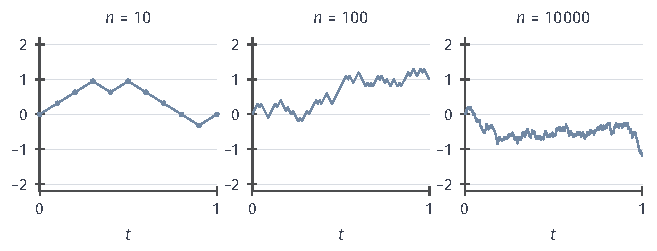
\includegraphics[width=111mm]{figures/03-optimization-evolution-and-signals/02-processes-and-trajectory-evolution/tikz/ctsp-donsker/figure.pdf}
  \caption{Donsker缩放。用同一列$10000$个独立等可能的$\pm1$步长（固定随机种子），分别取前$n=10,100,10000$步，画出$k/n\mapsto S_k/\sqrt n$的线性插值。纵向按$\sqrt n$、横向按$n$缩放后，三条折线的起伏幅度相当；$n$增大时局部锯齿变细，路径规律趋于Brownian运动。}
  \label{fig:ctsp-donsker}
\end{figure}

过程收敛加上连续映射，给出了离散问题的近似答案。例如
\[
  \max_{k\leq n}S_k/\sqrt n=\max_tX_n(t)\Rightarrow\max_{t\leq1}W_t ,
\]
由反射原理~\eqref{eq:ctsp-reflection}，
\[
  \mathbb P\Bigl(\max_{k\leq n}S_k\geq a\sqrt n\Bigr)\to2\bigl[1-\Phi(a)\bigr],\qquad a>0 .
\]
单时刻的中心极限定理只给出$S_n/\sqrt n$的分布，无法回答关于最大值的问题；这里需要的正是整条路径的收敛。

\paragraph{一般微小增量的扩散近似}
Donsker定理的增量独立同分布、条件均值为零。更一般的Markov链每一步的增量可以依赖当前状态，并且有小的漂移。设对每个$n$，$(X^n_k)_k$是Markov链，记增量$\Delta^n_k=X^n_{k+1}-X^n_k$，并在时间尺度$t=k/n$上观察。若在每个紧集上一致地有
\[
  \begin{aligned}
    n\,\mathbb E[\Delta^n_k\mid X^n_k=x]&\to b(x),\\
    n\,\mathbb E[(\Delta^n_k)^2\mid X^n_k=x]&\to a(x),\\
    n\,\mathbb E[|\Delta^n_k|^{2+\delta}\mid X^n_k=x]&\to0
  \end{aligned}
\]
（最后一条是Lindeberg型条件，排除单步的大跳跃），初值收敛，路径在有界时间内以高概率停留在紧集中，并且以$b$为漂移、$a$为扩散系数的鞅问题适定，那么$X^n_{\lfloor nt\rfloor}$收敛到相应的扩散\scite{math-kallenberg2021probability}。这类结论统称\term{扩散近似}（diffusion approximation）。漂移与扩散系数分别来自条件均值与条件二阶矩，乘以$n$是因为每单位时间有$n$步。

\begin{example}[Wright--Fisher扩散]
  \label{ex:ctsp-wright-fisher}
  规模为$n$的群体中某个等位基因的频率为$p$，下一代的$n$个个体独立地以概率$p$携带该基因，于是下一代频率是$\operatorname{Binomial}(n,p)/n$。增量的条件均值为$0$，条件方差为$p(1-p)/n$，四阶矩为$O(n^{-2})$。以$n$代为一个时间单位，条件均值与方差乘以$n$后分别为$0$与$p(1-p)$。频率过程收敛到扩散$\mathrm dX=\sqrt{X(1-X)}\,\mathrm dW$。它在$0$与$1$处噪声消失，这两个点是吸收态，与第~\ref{sec:ctsp-invariant}节讨论的不变分布不唯一的例子同类：基因最终要么消失，要么固定。
\end{example}

\paragraph{与平均ODE的对照}
扩散近似与第~\ref{chap:discrete-time-stochastic-processes}章随机逼近的平均ODE都描述“步长很小的随机递推”，但它们看的是不同的尺度，结论不能互换。以常步长$a$的递推$\theta_{k+1}=\theta_k+a[h(\theta_k)+\xi_{k+1}]$为例，$\xi$为条件方差$\sigma^2$的鞅差。在算法时间$t=ka$上观察，每单位时间有$1/a$步，条件均值乘以$1/a$得$h$，条件方差乘以$1/a$得$a\sigma^2\to0$。所以$a\to0$时，路径收敛到平均ODE $\dot\theta=h(\theta)$：噪声在这个尺度下消失。

若把偏离ODE轨迹的部分按$\sqrt a$放大，即考虑$(\theta_{\lfloor t/a\rfloor}-\bar\theta(t))/\sqrt a$，其中$\bar\theta$是ODE的解，噪声就重新以有限的强度出现，在适当条件下这一放大的偏差收敛到一个线性扩散（ODE附近的OU型过程）。前者回答“递推平均地往哪里走”，后者回答“围绕平均路径的波动有多大”。第~\ref{sec:ctsp-sa-lyapunov}节常增益情形的稳态方差$a\sigma^2/2$正是这种$\sqrt a$量级的波动。只改变记号而不改变尺度，就会把一种极限的结论误用到另一种上。

\section{本章小结}
\label{sec:ctsp-summary}

本章开头的三台记录仪分别给出跳跃路径、连续抖动的路径，以及噪声与状态相互作用的路径。回头看，它们沿着“路径—条件未来—累计与停止—状态方程—分布与长期行为—近似”这条线得到了处理，每一步都与上一章的离散时间结论对应，又都补上了连续时间特有的条件。

路径层面，Poisson过程由独立指数等待时间构造，Brownian运动由独立高斯增量与连续版本定义。时间连续并不意味着路径连续：前者是右连续有左极限的跳跃路径，后者处处连续而总变差无限、二次变差等于时间。不可数时刻带来的问题由三项约定解决：取右连续有左极限的版本，使修改与不可区分在其中一致；使用满足通常条件的滤过；以每个实数时刻上可判断的停时，并用二进上逼近把离散结论搬过来。

条件结构有两种，它们可以在同一个过程上同时成立。Markov性质由转移半群描述，半群又由生成元这一短时间变化率决定；连续时间Markov链把这些对象变成矩阵，但可数状态时还要检查不爆炸，强Markov性质还需要路径与Feller正则性。鞅性质约束条件均值；可选抽样、Doob最大不等式与鞅收敛都在右连续版本上成立，无界停时仍要一致可积，局部鞅取期望之前要验证可积性。计数过程扣除可预测的补偿量后才是鞅。

累计与状态方程是本章新增的核心。对时间与有限次跳跃可以逐路径累计，跳跃系数必须可预测；对Brownian运动只能借Itô等距在$L^2$中构造积分。二次变差使Itô公式多出$\frac12\operatorname{tr}(\bm\sigma\bm\sigma^\top\nabla^2V)$，跳跃则保留完整的有限差；Stratonovich约定恢复普通链式法则，但与Itô约定之间的转换要修正漂移。随机微分方程在全局Lipschitz条件下由Picard迭代得到强解，局部条件下需要Lyapunov函数排除爆炸；几何Brownian运动、OU过程与线性系统给出了可以直接核对的显式解。

从路径到整体规律的桥梁是生成元。Dynkin公式与含时间的Itô公式把期望、密度与首次到达化为后向方程、Fokker--Planck方程与边值问题，Feynman--Kac公式又把一类线性PDE的解写成路径期望。长期行为需要区分两个问题：同一噪声下的路径是否稳定，以及分布是否趋于不变分布。乘性噪声说明几乎必然稳定与均方稳定可以不一致；形式稳态密度只是候选，存在、唯一与收敛要分别论证；时间平均的误差由长期方差或Poisson方程控制，遍历性本身不保证中心极限定理。

表~\ref{tab:ctsp-discrete-continuous}把这些对应关系集中列出。

\begin{table*}[htbp]
  \centering
  \begin{tabularx}{\linewidth}{@{}l>{\RaggedRight\arraybackslash}p{50mm}>{\RaggedRight\arraybackslash}X@{}}
    \toprule
    问题 & 离散时间（第~\ref{chap:discrete-time-stochastic-processes}章） & 连续时间新增的对象与条件\\
    \midrule
    怎样生成路径 & 转移矩阵、转移核、随机递推 & 等待时间与跳转率；Brownian增量与连续版本；随机微分方程\\
    条件未来 & 多步核、Chapman--Kolmogorov & 转移半群与生成元的定义域；不爆炸；强Markov需路径与Feller正则\\
    累计与停止 & 鞅变换、可选抽样、Doob不等式 & 右连续版本、二进逼近、局部化；可预测补偿；Itô积分与二次变差\\
    分布演化 & 分布右乘转移核 & 弱形式、Fokker--Planck方程（需密度正则）、后向方程与边值问题\\
    长期行为 & 不变分布、遍历平均、相关误差 & 半群不动点、骨架链与连续过程的区别、Poisson方程与长期方差\\
    近似与计算 & 有限步偏差、平均误差 & 强误差与弱误差、事件驱动模拟、步长偏差、路径空间紧性\\
    \bottomrule
  \end{tabularx}
  \caption{离散时间与连续时间随机过程的对应。右列只列出连续时间新增的对象与条件，离散时间的定义与结论在相应位置简短回顾后沿用。}
  \label{tab:ctsp-discrete-continuous}
\end{table*}

最后三类计算任务使用相同的工具，目标却不同，应当分开理解。数值模拟忠实地近似一个给定的模型，误差按路径或期望衡量，并且有限时段的误差界不能直接推出长期行为。采样积分设计一个以目标分布为不变分布的过程，要求它长期保持非退化的随机性，按停留时间累计平均；离散化会改变不变分布，需要接受校正或步长控制。连续时间随机逼近则让增益递减、噪声逐渐压低，使状态收敛到指定的根；在算法时钟下它接近平均ODE，放大波动后又呈现扩散的形态。Itô积分是这三者共同的分析工具，而不是它们要计算的数值积分。

路径极限理论为离散近似与连续模型之间的关系提供了最后的依据：有限维分布收敛加上路径紧性，才能推出整条路径的分布收敛，并经连续映射传给最大值、时间积分与首次到达等泛函。

